% Problems, Chapter 18: More Special Functions
% Arfken, Weber & Harris, Mathematical Methods for Physicists, 7th ed.
% Requires: amsmath, amssymb, tikz

\section*{Problems}

\erratum{Unless an exercise says otherwise, polynomial degrees and
derivative orders in this chapter are nonnegative integers.  The
associated Laguerre index $k$ is a fixed nonnegative integer.  Real
and complex extensions are stated separately where needed.}

\Needspace{12\baselineskip}
\subsection*{18.1 Hermite Functions}

\Needspace{5\baselineskip}
\par\bigskip
\noindent\textbf{18.1.1}\quad Assume that the Hermite polynomials are
known to be solutions of the Hermite ODE, Eq.~(18.1). Assume further
that the recurrence relation, Eq.~(18.3), and the values of $H_{n}(0)$
are also known. Given the existence of a generating function
\[
g(x,t)=\sum_{n=0}^{\infty}H_{n}(x)\,\frac{t^{n}}{n!},
\]
\begin{enumerate}
\item[(a)] Differentiate $g(x,t)$ with respect to $x$ and using the
recurrence relation develop a first-order PDE for $g(x,t)$.
\item[(b)] Integrate with respect to $x$, holding $t$ fixed.
\item[(c)] Evaluate $g(0,t)$ using the known values of $H_{n}(0)$.
\item[(d)] Finally, show that $g(x,t)=\exp(-t^{2}+2tx)$.
\end{enumerate}
\solution
\erratum{The Instructor's Manual prints $g(x,0)=f(t)$ in part (c); the
evaluation is $g(0,t)=f(t)$, because $g=e^{2tx}f(t)$ from part (b) reduces
to $f(t)$ at $x=0$.}\par

First derive the derivative identity from precisely the stated data.
Write $D=d/dx$ and $L_n=D^2-2xD+2n$, so that the ODE reads $L_mH_m=0$.
Since $L_n=L_m+2(n-m)$, the ODE gives
\[
L_nH_{n+1}=-2H_{n+1},\qquad L_nH_{n-1}=2H_{n-1},
\]
while the product rule, $D(xH_n)=xH_n'+H_n$ and
$D^2(xH_n)=xH_n''+2H_n'$, gives
\[
L_n(xH_n)=xL_nH_n+2H_n'-2xH_n=2H_n'-2xH_n.
\]
Apply $L_n$ to the known identity
$H_{n+1}-2xH_n+2nH_{n-1}=0$, and then use the same identity to
replace $H_{n+1}$:
\begin{align*}
0&=-2H_{n+1}-4H_n'+4xH_n+4nH_{n-1}\\
 &=-2(2xH_n-2nH_{n-1})-4H_n'+4xH_n+4nH_{n-1}\\
 &=8nH_{n-1}-4H_n'.
\end{align*}
Thus $H_n'=2nH_{n-1}$ for $n\ge1$; $H_0'=0$ because $H_0$, the
polynomial solution of degree zero, is the constant $H_0(0)=1$.  We have
not assumed the derivative formula separately.

(a) Differentiate the proposed generating series, initially as a
formal power series.  With $2n/n!=2/(n-1)!$ and $m=n-1$,
\[
\frac{\partial g}{\partial x}
 =\sum_{n=1}^\infty2nH_{n-1}(x)\frac{t^n}{n!}
 =2t\sum_{m=0}^\infty H_m(x)\frac{t^m}{m!}
 =\boxed{2tg}.
\]
(b) Holding $t$ fixed,
$\partial_x(e^{-2tx}g)=e^{-2tx}(\partial_xg-2tg)=0$, so $e^{-2tx}g$
depends on $t$ alone, say $f(t)$, and $g(x,t)=e^{2tx}f(t)$.

(c) At $x=0$, the known values are
$H_{2m}(0)=(-1)^m(2m)!/m!$ and $H_{2m+1}(0)=0$.  Therefore
\[
f(t)=g(0,t)=\sum_{m=0}^\infty
 \frac{(-1)^m(2m)!}{m!}\frac{t^{2m}}{(2m)!}
 =\sum_{m=0}^\infty\frac{(-t^2)^m}{m!}=e^{-t^2}.
\]
(d) Substitution gives
\[
\boxed{g(x,t)=e^{2tx-t^2}}.
\]
The resulting exponential is entire in $t$ for each $x$, so its
coefficient identity also establishes convergence of the initially
formal generating series everywhere.

\Needspace{5\baselineskip}
\par\bigskip
\noindent\textbf{18.1.2}\quad In developing the properties of the
Hermite polynomials, start at a number of different points, such as:
\begin{enumerate}
\item[1.] Hermite's ODE, Eq.~(18.1),
\item[2.] Rodrigues's formula, Eq.~(18.8),
\item[3.] Integral representation, Eq.~(18.10),
\item[4.] Generating function, Eq.~(18.2),
\item[5.] Gram--Schmidt construction of a complete set of orthogonal
polynomials over $(-\infty,\infty)$ with a weighting factor of
$\exp(-x^{2})$ (Section~5.2).
\end{enumerate}
Outline how you can go from any one of these starting points to all
the other points.
\erratum{In the ODE and Gram--Schmidt constructions, select the degree-$n$ polynomial with leading coefficient $2^n$.}\par\nobreak
\solution
\erratum{To identify a unique Hermite polynomial, supplement the ODE
or Gram--Schmidt construction by degree $n$ and leading coefficient
$2^n$.  The ODE alone also has nonpolynomial solutions, and orthogonality
alone does not fix the scale.}
Here is a closed chain, with both directions to the fifth starting point.

\textit{ODE $\longrightarrow$ Rodrigues.}
Let $w=e^{-x^2}$ and $D=d/dx$.  Differentiating $w'+2xw=0$ exactly
$n+1$ times, with Leibniz's rule $D^{n+1}(xw)=xw^{(n+1)}+(n+1)w^{(n)}$, gives
\[
w^{(n+2)}+2xw^{(n+1)}+2(n+1)w^{(n)}=0.
\]
Put $w^{(n)}=(-1)^nwR_n$.  Since $w'=-2xw$, the product rule gives
\begin{align*}
w^{(n+1)}&=(-1)^nw(R_n'-2xR_n),\\
w^{(n+2)}&=(-1)^nw\bigl[R_n''-2xR_n'-2R_n-2x(R_n'-2xR_n)\bigr]\\
 &=(-1)^nw\bigl[R_n''-4xR_n'+(4x^2-2)R_n\bigr].
\end{align*}
Substitution into the differentiated equation and division by
$(-1)^nw$ give
\begin{align*}
0={}&R_n''-4xR_n'+(4x^2-2)R_n
       +2x(R_n'-2xR_n)+2(n+1)R_n\\
 ={}&R_n''-2xR_n'+2nR_n.
\end{align*}
Differentiation of $w$ repeatedly produces $w$ times a polynomial, since
$D(wp)=w(p'-2xp)$; each step multiplies the highest term by $-2x$, so
the highest term of $w^{(n)}/w$ is $(-2x)^n$.  Thus $R_n$ has degree $n$
and leading coefficient $(-1)^n(-2)^n=2^n$.  Two such polynomial
solutions differ by a polynomial $d$ of degree below $n$ with $L_nd=0$,
where $L_n=D^2-2xD+2n$.  If $d\ne0$, let $cx^m$, with $c\ne0$ and
$m<n$, be its leading term.  The $x^m$ term of $L_nd$ is then
$(-2m+2n)cx^m\ne0$, because $D^2$ lowers the degree, contradicting
$L_nd=0$.  Hence $d=0$ and
\[
H_n=R_n=(-1)^ne^{x^2}\frac{d^n}{dx^n}e^{-x^2}.
\]

\textit{Rodrigues $\longrightarrow$ generating function.}
Taylor's theorem for the entire function $w$ gives
\[
\sum_{n=0}^\infty H_n(x)\frac{t^n}{n!}
 =e^{x^2}\sum_{n=0}^\infty\frac{(-t)^n}{n!}w^{(n)}(x)
 =e^{x^2}w(x-t)=e^{x^2-(x-t)^2}=e^{-t^2+2xt}.
\]

\textit{Generating function $\longleftrightarrow$ contour integral.}
Cauchy's coefficient formula on a positively oriented circle about zero is
\[
H_n(x)=\frac{n!}{2\pi i}\oint_{|z|=R}
 \frac{e^{-z^2+2xz}}{z^{n+1}}\,dz.
\]
Conversely, multiply by $t^n/n!$ and sum for $|t|<R$.
The geometric series $\sum_nt^n/z^{n+1}=1/(z-t)$ converges uniformly on
that circle, so termwise integration and Cauchy's integral formula give
\[
\sum_{n=0}^\infty H_n(x)\frac{t^n}{n!}
 =\frac1{2\pi i}\oint\frac{e^{-z^2+2xz}}{z-t}\,dz
 =e^{-t^2+2xt}.
\]
Any fixed $t$ is covered by choosing $R>|t|$.

\textit{Generating function $\longrightarrow$ ODE.}
For $g=e^{-t^2+2xt}$, direct differentiation gives $g_x=2tg$,
$g_{xx}=4t^2g$ and $g_t=(2x-2t)g$, so
\[
g_{xx}-2xg_x+2tg_t
 =[4t^2-4xt+2t(2x-2t)]g=0.
\]
Since $t\,\partial_t(t^n/n!)=nt^n/n!$, the $t^n/n!$ coefficient of this
equation is $H_n''-2xH_n'+2nH_n=0$.
These coefficients are polynomials of degree $n$ with leading
coefficient $2^n$, as the uniqueness argument in
\textit{ODE $\longrightarrow$ Rodrigues} requires: multiplying
$e^{2xt}=\sum_j(2x)^jt^j/j!$ by $e^{-t^2}=\sum_k(-1)^kt^{2k}/k!$ and
collecting the terms with $j+2k=n$ give the coefficient of $t^n/n!$,
\[
H_n(x)=n!\sum_{k=0}^{\lfloor n/2\rfloor}
 \frac{(-1)^k(2x)^{n-2k}}{k!\,(n-2k)!},
\]
whose highest term, from $k=0$, is $(2x)^n$.
This closes the first four starting points.

\textit{Rodrigues $\longleftrightarrow$ Gram--Schmidt.}
For every polynomial $q$ of degree less than $n$, use $wH_n=(-1)^nw^{(n)}$
and integrate by parts $n$ times; each integration moves one derivative
onto $q$ with a factor $-1$:
\[
\int_{-\infty}^{\infty}wH_nq\,dx
 =(-1)^n\int_{-\infty}^{\infty}w^{(n)}q\,dx
 =\int_{-\infty}^{\infty}wq^{(n)}\,dx=0.
\]
Every boundary term is a polynomial times $e^{-x^2}$ and vanishes.
For $q=H_n$, whose leading term is $2^nx^n$, the $n$th derivative is
$2^nn!$, so the same calculation and $\int w\,dx=\sqrt\pi$ give
\[
\int_{-\infty}^{\infty}wH_n^2\,dx=2^nn!\sqrt\pi.
\]
Therefore Rodrigues produces the orthogonal polynomials generated by
Gram--Schmidt from $1,x,x^2,\ldots$, with the prescribed leading coefficients.
Conversely, two degree-$n$ polynomials with that leading coefficient and
orthogonality to all lower degrees have difference $d$ of degree below
$n$.  Orthogonality gives $\int w d^2=0$, hence $d=0$.  Thus Gram--Schmidt
recovers Rodrigues and enters the preceding chain.

Completeness in $L^2(\mathbb R,w\,dx)$ can also be justified.  If $f$
is orthogonal to every polynomial, set
$F(z)=\int_{\mathbb R}f(x)w(x)e^{zx}\,dx$.
Cauchy--Schwarz bounds this integral and all its differentiated integrals
uniformly on compact $z$ sets by Gaussian moments, so $F$ is entire.
All $F^{(n)}(0)=\int_{\mathbb R}f(x)w(x)x^n\,dx$ vanish, so the Taylor
series of $F$ about zero vanishes, implying $F=0$.  In particular the Fourier
transform of the integrable function $fw$ is zero; Fourier uniqueness
gives $fw=0$ almost everywhere, hence $f=0$.

\Needspace{5\baselineskip}
\par\bigskip
\noindent\textbf{18.1.3}\quad Prove that
$\big|H_{n}(x)\big| \le \big|H_{n}(ix)\big|$.
\erratum{Take $x$ real.}\par\nobreak
\solution
\erratum{The assertion is for real $x$.  It is false for arbitrary
complex $x$: for $n=2$, $x=i$, the two moduli are $6$ and $2$.}
The finite series is
\[
H_n(x)=n!\sum_{k=0}^{\lfloor n/2\rfloor}
 \frac{(-1)^k(2x)^{n-2k}}{k!(n-2k)!}.
\]
For real $x$, the triangle inequality gives
\[
|H_n(x)|\le n!\sum_{k=0}^{\lfloor n/2\rfloor}
 \frac{(2|x|)^{n-2k}}{k!(n-2k)!}.
\]
On the other hand $(-1)^ki^{n-2k}=i^n(-1)^k(i^2)^{-k}=i^n$, so
\[
H_n(ix)=i^nn!\sum_{k=0}^{\lfloor n/2\rfloor}
 \frac{(2x)^{n-2k}}{k!(n-2k)!}.
\]
The exponents $n-2k$ all have the parity of $n$.  For $x>0$
all terms are nonnegative; for $x<0$ they all have the sign $(-1)^n$.
No cancellation occurs, so
\[
|H_n(ix)|=n!\sum_{k=0}^{\lfloor n/2\rfloor}
 \frac{(2|x|)^{n-2k}}{k!(n-2k)!},
\]
which is exactly the bound just obtained for $|H_n(x)|$.
At $x=0$ the conclusion follows directly from the constant terms.
Thus $\boxed{|H_n(x)|\le|H_n(ix)|}$ for every real $x$.

\Needspace{5\baselineskip}
\par\bigskip
\noindent\textbf{18.1.4}\quad Rewrite the series form of $H_{n}(x)$,
Eq.~(18.9), as an ascending power series.
\par\nobreak\hfill\emph{ANS.}\enspace
$H_{2n}(x)=(-1)^{n}\displaystyle\sum_{s=0}^{n}
(-1)^{\erratum{s}}(2x)^{2s}\frac{(2n)!}{(2s)!\,(n-s)!}$,\par\nobreak
\hfill$H_{2n+1}(x)=(-1)^{n}\displaystyle\sum_{s=0}^{n}
(-1)^{s}(2x)^{2s+1}\frac{(2n+1)!}{(2s+1)!\,(n-s)!}$.
\solution
Start with the descending series
$H_N(x)=N!\sum_{k=0}^{\lfloor N/2\rfloor}
(-1)^k(2x)^{N-2k}/[k!(N-2k)!]$.
For $N=2n$, put $s=n-k$, so $k=n-s$ and $N-2k=2s$.  As $k$ goes from
$0$ to $n$, $s$ goes from $n$ to $0$, and reversing the finite sum and
using $(-1)^{n-s}=(-1)^n(-1)^s$ give
\begin{align*}
H_{2n}(x)
 &=(2n)!\sum_{s=0}^n
 \frac{(-1)^{n-s}(2x)^{2s}}{(n-s)!(2s)!}\\
 &=\boxed{(-1)^n\sum_{s=0}^n
 \frac{(-1)^s(2n)!(2x)^{2s}}{(2s)!(n-s)!}}.
\end{align*}
For $N=2n+1$ we have $\lfloor N/2\rfloor=n$, and the same change
$s=n-k$ gives $N-2k=2s+1$, hence
\begin{align*}
H_{2n+1}(x)
 &=(2n+1)!\sum_{s=0}^n
 \frac{(-1)^{n-s}(2x)^{2s+1}}{(n-s)!(2s+1)!}\\
 &=\boxed{(-1)^n\sum_{s=0}^n
 \frac{(-1)^s(2n+1)!(2x)^{2s+1}}{(2s+1)!(n-s)!}}.
\end{align*}
\erratum{The even formula needs $(-1)^s$, not the textbook's
$(-1)^{2s}$.}  For example the corrected $n=1$ formula gives
$H_2(x)=4x^2-2$, directly checking the relative sign.

\Needspace{5\baselineskip}
\par\bigskip
\noindent\textbf{18.1.5}
\begin{enumerate}
\item[(a)] Expand $x^{2r}$ in a series of even-order Hermite
polynomials.
\item[(b)] Expand $x^{2r+1}$ in a series of odd-order Hermite
polynomials.
\end{enumerate}
\par\nobreak\hfill\emph{ANS.}\enspace
(a) $x^{2r}=\dfrac{(2r)!}{2^{2r}}\displaystyle\sum_{n=0}^{r}
\dfrac{H_{2n}(x)}{(2n)!\,(r-n)!}$\par\nobreak
\hfill(b) $x^{2r+1}=\dfrac{(2r+1)!}{2^{2r+1}}
\displaystyle\sum_{n=0}^{r}\dfrac{H_{2n+1}(x)}{(2n+1)!\,(r-n)!}$,
\qquad $r=0,1,2,\ldots.$
\par\emph{Hint.}~Use a Rodrigues representation and integrate by
parts.
\solution
Because $H_n$ has degree $n$ and leading coefficient $2^n$, the
polynomials $H_0,\ldots,H_m$ form a basis for polynomials of degree
at most $m$.  Write $x^m=\sum_{n=0}^m c_nH_n(x)$.  Orthogonality gives
\[
c_n=\frac1{2^nn!\sqrt\pi}
 \int_{-\infty}^{\infty}x^me^{-x^2}H_n(x)\,dx.
\]
By Rodrigues's formula $e^{-x^2}H_n=(-1)^nD^ne^{-x^2}$, with $D=d/dx$.
Each of $n$ integrations by parts moves one derivative onto $x^m$ with a
factor $-1$, and every boundary term is a polynomial times a derivative
of $e^{-x^2}$, which vanishes at $\pm\infty$.  Since
$D^nx^m=m!\,x^{m-n}/(m-n)!$ for $n\le m$,
\begin{align*}
\int_{-\infty}^{\infty}x^me^{-x^2}H_n(x)\,dx
 &=(-1)^n\int_{-\infty}^{\infty}x^mD^ne^{-x^2}\,dx
 =\int_{-\infty}^{\infty}e^{-x^2}D^nx^m\,dx\\
 &=\frac{m!}{(m-n)!}\int_{-\infty}^{\infty}x^{m-n}e^{-x^2}\,dx.
\end{align*}
Odd powers integrate to zero, the integrand being odd.  For $m-n=2j$,
the integrand is even, and the substitution $u=x^2$, $dx=du/(2\sqrt u)$,
gives
\[
\int_{-\infty}^{\infty}x^{2j}e^{-x^2}\,dx
 =2\int_0^\infty x^{2j}e^{-x^2}\,dx
 =\int_0^\infty u^{j-1/2}e^{-u}\,du
 =\Gamma(j+\tfrac12)=\frac{(2j)!\sqrt\pi}{4^jj!}.
\]
The last value follows from
$\Gamma(j+\frac12)=(j-\frac12)(j-\frac32)\cdots\frac12\,\Gamma(\frac12)
=2^{-j}(2j-1)!!\sqrt\pi$ and $(2j-1)!!=(2j)!/(2^jj!)$.
Consequently, with $(m-n)!=(2j)!$ and $2^n4^j=2^{n+2j}=2^m$,
\[
c_n=\frac1{2^nn!\sqrt\pi}\,\frac{m!}{(2j)!}\,
 \frac{(2j)!\sqrt\pi}{4^jj!}
 =\frac{m!}{2^n4^jn!j!}
 =\frac{m!}{2^mn!j!},\qquad n=m-2j,
\]
and $c_n=0$ when $m-n$ is odd.

(a) Take $m=2r$; only even $n=2k$ contribute, with $j=r-k$:
\[
\boxed{x^{2r}=\frac{(2r)!}{2^{2r}}
 \sum_{k=0}^r\frac{H_{2k}(x)}{(2k)!(r-k)!}}.
\]
(b) Take $m=2r+1$; only odd $n=2k+1$ contribute, again with $j=r-k$:
\[
\boxed{x^{2r+1}=\frac{(2r+1)!}{2^{2r+1}}
 \sum_{k=0}^r\frac{H_{2k+1}(x)}{(2k+1)!(r-k)!}}.
\]
These finite identities include $r=0$, giving $1=H_0$ and $x=H_1/2$.

\Needspace{5\baselineskip}
\par\bigskip
\noindent\textbf{18.1.6}\quad Show that
\begin{enumerate}
\item[(a)] $\displaystyle\int_{-\infty}^{\infty}
H_{n}(x)\exp\left[-\frac{x^{2}}{2}\right]dx
=\begin{cases}
\erratum{\sqrt{2\pi}}\,n!/(n/2)!, & n\text{ even},\\
0, & n\text{ odd}.
\end{cases}$
\item[(b)] $\displaystyle\int_{-\infty}^{\infty}
xH_{n}(x)\exp\left[-\frac{x^{2}}{2}\right]dx
=\begin{cases}
0, & n\text{ even},\\[8pt]
\erratum{\sqrt{2\pi}}\,\dfrac{(n+1)!}{((n+1)/2)!}, & n\text{ odd}.
\end{cases}$
\end{enumerate}
\solution
(a) Multiply the generating function by $e^{-x^2/2}$ and integrate.
For real $t$, completion of the square,
$-\tfrac12x^2+2tx-t^2=-\tfrac12(x-2t)^2+t^2$, and the shift
$x\to x+2t$ give
\begin{align*}
\sum_{n=0}^\infty\frac{t^n}{n!}
 \int_{-\infty}^{\infty}e^{-x^2/2}H_n(x)\,dx
 &=\int_{-\infty}^{\infty}e^{-x^2/2+2tx-t^2}\,dx\\
 &=e^{t^2}\int_{-\infty}^{\infty}e^{-(x-2t)^2/2}\,dx\\
 &=\sqrt{2\pi}\,e^{t^2}
 =\sqrt{2\pi}\sum_{k=0}^\infty\frac{t^{2k}}{k!}.
\end{align*}
The right side contains only even powers, and
$t^{2k}/k!=[(2k)!/k!]\,t^{2k}/(2k)!$.  Comparing coefficients of
$t^n/n!$ (with $n=2k$ for even $n$) gives
\[
\boxed{\int_{-\infty}^{\infty}e^{-x^2/2}H_n(x)\,dx
 =\begin{cases}\sqrt{2\pi}\,n!/(n/2)!,&n\text{ even},\\
 0,&n\text{ odd}.\end{cases}}
\]
The interchange of sum and integral is justified for $|t|\le R$ by
dominated convergence.  By Exercise 18.1.3, $|H_n(x)|\le|H_n(ix)|
=n!\sum_k(2|x|)^{n-2k}/[k!(n-2k)!]$, so, with $R^n=R^{n-2k}R^{2k}$,
\[
\sum_{n=0}^\infty|H_n(x)|\frac{R^n}{n!}
 \le\sum_{n=0}^\infty\sum_{k=0}^{\lfloor n/2\rfloor}
 \frac{(2R|x|)^{n-2k}R^{2k}}{k!(n-2k)!}
 =e^{2R|x|}e^{R^2},
\]
the double sum being the Cauchy product of the two exponential series.
Every partial sum is therefore bounded by the integrable function
$e^{R^2}e^{-x^2/2+2R|x|}$.

(b) Inserting $x$, completing the same square and putting $y=x-2t$ give
\begin{align*}
\sum_{n=0}^\infty\frac{t^n}{n!}
 \int_{-\infty}^{\infty}xe^{-x^2/2}H_n(x)\,dx
 &=e^{t^2}\int_{-\infty}^{\infty}(y+2t)e^{-y^2/2}\,dy\\
 &=2t\sqrt{2\pi}\,e^{t^2}
 =\sqrt{2\pi}\sum_{k=0}^\infty\frac{2t^{2k+1}}{k!}.
\end{align*}
The interchange of sum and integral is justified as in (a): for
$|t|\le R$ the partial sums are now bounded by
$|x|e^{R^2}e^{-x^2/2+2R|x|}$, which is still integrable.
The odd Gaussian moment $\int ye^{-y^2/2}dy$ is zero, and
$2t\int e^{-y^2/2}dy=2t\sqrt{2\pi}$.  The right side has only odd
powers, and
\[
\frac{2t^{2k+1}}{k!}=\frac{2(2k+1)!}{k!}\,\frac{t^{2k+1}}{(2k+1)!}.
\]
Thus even $n$ give zero, and for $n=2k+1$ the answer is
$\sqrt{2\pi}\,2(2k+1)!/k!$.  Since $2(2k+1)!/k!=(2k+2)(2k+1)!/[(k+1)k!]=(2k+2)!/(k+1)!$, this is
\[
\boxed{\int_{-\infty}^{\infty}xe^{-x^2/2}H_n(x)\,dx
 =\begin{cases}0,&n\text{ even},\\[3pt]
 \sqrt{2\pi}\,(n+1)!/((n+1)/2)!,&n\text{ odd}.
 \end{cases}}
\]
\erratum{Both square roots implement the published correction of
$2\pi$ to $\sqrt{2\pi}$.}  The case $n=0$ in (a) is the usual Gaussian
integral and already detects the original normalization error.

\Needspace{5\baselineskip}
\par\bigskip
\noindent\textbf{18.1.7}
\begin{enumerate}
\item[(a)] Using the Cauchy integral formula, develop an integral
representation of $H_{n}(x)$ based on Eq.~(18.2) with the contour
enclosing the point $z=-x$.
\par\nobreak\hfill\emph{ANS.}\enspace
$H_{n}(x)=\dfrac{n!}{2\pi i}\,e^{x^{2}}
\displaystyle\oint\frac{e^{-z^{2}}}{(z+x)^{n+1}}\,dz$.
\item[(b)] Show by direct substitution that this result satisfies the
Hermite equation.
\end{enumerate}
\solution
(a) Cauchy's coefficient formula applied to the generating function gives
\[
H_n(x)=\frac{n!}{2\pi i}\oint_{|w|=R}
 \frac{e^{-w^2+2xw}}{w^{n+1}}\,dw.
\]
Set $z=w-x$.  Then $w=z+x$, $dw=dz$, and
$-w^2+2xw=-(z+x)^2+2x(z+x)=x^2-z^2$.
The positively oriented circle now encloses $z=-x$, and hence
\[
\boxed{H_n(x)=\frac{n!}{2\pi i}e^{x^2}
 \oint\frac{e^{-z^2}}{(z+x)^{n+1}}\,dz}.
\]
Any positively oriented simple contour enclosing $-x$ gives the same
result, since this is the only finite singularity of the integrand.

(b) Use the original $w$ contour, which stays fixed as $x$ varies;
its integrand is entire in $x$, so differentiation under the finite
contour integral is valid.  Put $E=e^{-w^2+2xw}$, so that
$\partial_xE=2wE$.  Then
\[
H_n'=\frac{n!}{2\pi i}\oint\frac{2wE}{w^{n+1}}\,dw,
\qquad
H_n''=\frac{n!}{2\pi i}\oint\frac{4w^2E}{w^{n+1}}\,dw.
\]
Combining all three terms of the ODE gives
\begin{align*}
H_n''-2xH_n'+2nH_n
 &=\frac{n!}{2\pi i}\oint
 \frac{(4w^2-4xw+2n)E}{w^{n+1}}\,dw\\
 &=-2\,\frac{n!}{2\pi i}\oint
 \frac{d}{dw}\left(\frac{E}{w^n}\right)dw=0.
\end{align*}
Indeed, since $\partial_wE=(-2w+2x)E$,
\[
\frac{d}{dw}\left(\frac{E}{w^n}\right)
 =\frac{(-2w+2x)E}{w^n}-\frac{nE}{w^{n+1}}
 =\frac{(-2w^2+2xw-n)E}{w^{n+1}},
\]
and multiplication by $-2$ gives precisely the numerator
$4w^2-4xw+2n$.  The integral of this derivative is zero
because its primitive is single-valued on the closed contour, even
though it can have a pole inside.  This proves the equation directly,
including $n=0$.

\Needspace{12\baselineskip}
\subsection*{18.2 Applications of Hermite Functions}

\Needspace{5\baselineskip}
\par\bigskip
\noindent\textbf{18.2.1}\quad Prove that
$\left(2x-\dfrac{d}{dx}\right)^{n}1=H_{n}(x)$.
\par\emph{Hint.}~Check out the cases $n=0$ and $n=1$ and then use
mathematical induction (Section~1.4).
\solution
Let $A=2x-D$, where $D=d/dx$ acts on everything to its right.
The derivative formula $H_n'=2nH_{n-1}$ and the recurrence (18.3),
$H_{n+1}=2xH_n-2nH_{n-1}$, give
\[
AH_n=2xH_n-H_n'=2xH_n-2nH_{n-1}=H_{n+1}.
\]
Now $A^01=1=H_0$ and $A1=2x=H_1$.  If $A^n1=H_n$, then
\[
A^{n+1}1=A(A^n1)=AH_n=H_{n+1}.
\]
Mathematical induction therefore proves
$\boxed{(2x-D)^n1=H_n(x)}$ for every nonnegative integer $n$.
The operator power means repeated composition; $x$ and $D$ do not
commute, since $D(xf)=f+xDf$.

\Needspace{5\baselineskip}
\par\bigskip
\noindent\textbf{18.2.2}\quad Show that
$\displaystyle\int_{-\infty}^{\infty}x^{m}e^{-x^{2}}H_{n}(x)\,dx=0$
for $m$ an integer, $0\le m\le n-1$.
\solution
\erratum{The Instructor's Manual's polynomial expansion must start at
$H_0$, not $H_1$; its final integral is zero.  For example, the constant
polynomial cannot be expanded using only $H_1,\ldots,H_m$.}\par

For integers $0\le m<n$, Rodrigues gives
\begin{align*}
\int_{-\infty}^{\infty}x^me^{-x^2}H_n(x)\,dx
 &=(-1)^n\int_{-\infty}^{\infty}x^m
           \frac{d^n}{dx^n}e^{-x^2}\,dx\\
 &=\int_{-\infty}^{\infty}e^{-x^2}
           \frac{d^n}{dx^n}x^m\,dx=\boxed{0}.
\end{align*}
There are $n$ integrations by parts: their $(-1)^n$ cancels the
Rodrigues sign.  The $(i+1)$st of them, $0\le i<n$, reads
\begin{align*}
\int_{-\infty}^{\infty}(D^ix^m)\,D^{n-i}e^{-x^2}\,dx
 ={}&\Bigl[(D^ix^m)\,D^{n-i-1}e^{-x^2}\Bigr]_{-\infty}^{\infty}\\
 &-\int_{-\infty}^{\infty}(D^{i+1}x^m)\,D^{n-i-1}e^{-x^2}\,dx,
\end{align*}
with $D=d/dx$.  Every boundary term is a polynomial times a derivative
of the Gaussian, hence a polynomial times $e^{-x^2}$, and vanishes at
both infinities.  Finally
$D^nx^m=0$ because $n>m$.  For $n=0$ no integer $m$ meets the stated
range, so there is no exceptional missing case.

\Needspace{5\baselineskip}
\par\bigskip
\noindent\textbf{18.2.3}\quad The transition probability between two
oscillator states $m$ and $n$ depends on
\[
\int_{-\infty}^{\infty}xe^{-x^{2}}H_{n}(x)H_{m}(x)\,dx.
\]
Show that this integral equals
$\pi^{1/2}2^{n-1}n!\,\delta_{m,n-1}+\pi^{1/2}2^{n}(n+1)!\,
\delta_{m,n+1}$. This result shows that such transitions can occur
only between states of adjacent energy levels, $m=n\pm1$.
\par\emph{Hint.}~Multiply the generating function, Eq.~(18.2), by
itself using two different sets of variables $(x,s)$ and $(x,t)$.
Alternatively, the factor $x$ may be eliminated by the recurrence
relation, Eq.~(18.3).
\solution
The recurrence relation can be solved for multiplication by $x$:
\[
xH_n=\tfrac12H_{n+1}+nH_{n-1}.
\]
Let $I_{nm}$ denote the integral, and use the orthogonality integral
$\int_{\mathbb R}e^{-x^2}H_jH_m\,dx=\sqrt\pi\,2^jj!\,\delta_{jm}$.
Multiplying the recurrence by $e^{-x^2}H_m$ and integrating yields
\begin{align*}
I_{nm}
 &=\tfrac12\int_{\mathbb R}e^{-x^2}H_{n+1}H_m\,dx
   +n\int_{\mathbb R}e^{-x^2}H_{n-1}H_m\,dx\\
 &=\tfrac12\sqrt\pi\,2^{n+1}(n+1)!\,\delta_{m,n+1}
   +n\sqrt\pi\,2^{n-1}(n-1)!\,\delta_{m,n-1}\\
 &=\boxed{\sqrt\pi\,2^{n-1}n!\,\delta_{m,n-1}
   +\sqrt\pi\,2^n(n+1)!\,\delta_{m,n+1}},
\end{align*}
since $\tfrac12\,2^{n+1}=2^n$ and $n\,(n-1)!=n!$.
For $n=0$, omit the lowering term before writing its factorial:
$xH_0=H_1/2$.  The final formula still applies because
$\delta_{m,-1}=0$ for nonnegative $m$.
Thus the position matrix element vanishes unless $m=n\pm1$.
Normalization of the wave functions changes its nonzero magnitude
but not these zeros, giving the stated adjacent-level selection rule.

\Needspace{5\baselineskip}
\par\bigskip
\noindent\textbf{18.2.4}\quad Show that
$\displaystyle\int_{-\infty}^{\infty}
x^{2}e^{-x^{2}}H_{n}(x)H_{n}(x)\,dx
=\pi^{1/2}2^{n}n!\left(n+\frac{1}{2}\right)$.
This integral occurs in the calculation of the mean-square
displacement of our quantum oscillator.
\par\emph{Hint.}~Use the recurrence relation, Eq.~(18.3), and the
orthogonality integral.
\solution
Square $xH_n=H_{n+1}/2+nH_{n-1}$,
\[
x^2H_n^2=\tfrac14H_{n+1}^2+nH_{n+1}H_{n-1}+n^2H_{n-1}^2,
\]
and integrate with Gaussian weight, using the orthogonality integral:
\begin{align*}
\int_{\mathbb R}x^2e^{-x^2}H_n^2\,dx
 &=\frac14\int_{\mathbb R}e^{-x^2}H_{n+1}^2\,dx
   +n\int_{\mathbb R}e^{-x^2}H_{n+1}H_{n-1}\,dx
   +n^2\int_{\mathbb R}e^{-x^2}H_{n-1}^2\,dx\\
 &=\frac14\sqrt\pi\,2^{n+1}(n+1)!
   +n^2\sqrt\pi\,2^{n-1}(n-1)!\\
 &=\sqrt\pi\,2^{n-1}n![(n+1)+n]\\
 &=\boxed{\sqrt\pi\,2^nn!\left(n+\tfrac12\right)}.
\end{align*}
The mixed term is zero by orthogonality, and the third line uses
$\tfrac14\,2^{n+1}(n+1)!=2^{n-1}n!\,(n+1)$ and
$n^2\,2^{n-1}(n-1)!=2^{n-1}n!\,n$.  At $n=0$ the terms with
$H_{-1}$ are omitted at the first line, leaving $\sqrt\pi/2$;
this agrees with the final formula.  Dividing by the norm
$\sqrt\pi2^nn!$ gives $\langle x^2\rangle_n=n+1/2$ in the
dimensionless oscillator coordinate.

\Needspace{5\baselineskip}
\par\bigskip
\noindent\textbf{18.2.5}\quad Evaluate
\[
\int_{-\infty}^{\infty}x^{2}e^{-x^{2}}H_{n}(x)H_{m}(x)\,dx
\]
in terms of $n$ and $m$ and appropriate Kronecker delta functions.
\par\nobreak\hfill\emph{ANS.}\enspace
$2^{n-1}\pi^{1/2}(2n+1)n!\,\delta_{nm}
+2^{n}\pi^{1/2}(n+2)!\,\delta_{n+2,m}
+2^{n-2}\pi^{1/2}n!\,\delta_{n-2,m}$.
\solution
Apply the multiplication recurrence $xH_j=\frac12H_{j+1}+jH_{j-1}$
twice, first with $j=n$ and then with $j=n\pm1$, keeping each
coefficient:
\begin{align*}
x^2H_n
 &=\tfrac12xH_{n+1}+nxH_{n-1}\\
 &=\tfrac12\left(\tfrac12H_{n+2}+(n+1)H_n\right)
   +n\left(\tfrac12H_n+(n-1)H_{n-2}\right)\\
 &=\tfrac14H_{n+2}+\tfrac{2n+1}{2}H_n+n(n-1)H_{n-2}.
\end{align*}
Multiplication by $e^{-x^2}H_m$ and integration therefore gives
\begin{align*}
\int_{\mathbb R}x^2e^{-x^2}H_nH_m\,dx
 &=\tfrac14\sqrt\pi2^{n+2}(n+2)!\,\delta_{m,n+2}\\
 &\quad+\tfrac{2n+1}{2}\sqrt\pi2^nn!\,\delta_{mn}\\
 &\quad+n(n-1)\sqrt\pi2^{n-2}(n-2)!\,\delta_{m,n-2}\\
 &=\boxed{\begin{aligned}
 &\sqrt\pi2^{n-1}(2n+1)n!\,\delta_{mn}\\
 &{}+\sqrt\pi2^n(n+2)!\,\delta_{m,n+2}
   +\sqrt\pi2^{n-2}n!\,\delta_{m,n-2}
 \end{aligned}}.
\end{align*}
The orthogonality integral gives each line, and the box uses
$\tfrac14\,2^{n+2}=2^n$, $\tfrac{2n+1}{2}\,2^n=2^{n-1}(2n+1)$ and
$n(n-1)\,(n-2)!=n!$.
For $n=0,1$ the last Hermite term is absent; the last delta in the
boxed formula is zero for all allowed $m\ge0$, so that form covers
these cases without a negative factorial.  Setting $m=n$ recovers
Exercise 18.2.4.

\Needspace{5\baselineskip}
\par\bigskip
\noindent\textbf{18.2.6}\quad Show that
$\displaystyle\int_{-\infty}^{\infty}x^{r}e^{-x^{2}}
H_{n}(x)H_{n+p}(x)\,dx
=\begin{cases}
0, & p>r\\
2^{n}\pi^{1/2}(n+r)!, & p=r,
\end{cases}$
with $n$, $p$, and $r$ nonnegative integers.
\par\emph{Hint.}~Apply the multiplication recurrence, Eq.~(18.3), \erratum{$r$ times}, to $x^rH_n$.
\solution
\erratum{The recurrence removes one factor $x$ per application, so
$x^rH_n$ needs exactly $r$ applications, whatever the value of $p$;
this is the count in the corrected hint.}
Multiplication by $x$ raises a Hermite index by one with coefficient
$1/2$, or lowers it by one with coefficient equal to the current index:
$xH_j=H_{j+1}/2+jH_{j-1}$.  Iterating this relation $r$ times gives
\[
x^rH_n=2^{-r}H_{n+r}
       +\text{a polynomial of degree at most }n+r-2.
\]
To see why the highest coefficient is exactly $2^{-r}$, note that the only
way to reach index $n+r$ in $r$ steps is to raise the index at every
step; each contributes $1/2$.  Any lowering step decreases the final
index by two relative to that highest index.  This also follows by
matching leading terms: $x^rH_n$ has leading term $2^nx^{n+r}$,
whereas $H_{n+r}$ has leading term $2^{n+r}x^{n+r}$.

If $p>r$, the polynomial $x^rH_n$ has degree below $n+p$, so it is a
combination of $H_0,\ldots,H_{n+r}$ and is orthogonal to $H_{n+p}$.
If $p=r$, the lower terms, of degree at most $n+r-2$, are orthogonal
to $H_{n+r}$, and only the displayed highest Hermite term survives;
it contributes $2^{-r}\int e^{-x^2}H_{n+r}^2\,dx
=2^{-r}\sqrt\pi\,2^{n+r}(n+r)!$.  Consequently
\[
\boxed{\int_{-\infty}^{\infty}x^re^{-x^2}H_nH_{n+p}\,dx
 =\begin{cases}
 0,&p>r,\\
 2^{-r}\sqrt\pi2^{n+r}(n+r)!
 =2^n\sqrt\pi(n+r)!,&p=r.
 \end{cases}}
\]
The case $r=0,p=0$ is exactly the normalization integral.  All indices
are nonnegative integers as required by the question.

\Needspace{5\baselineskip}
\par\bigskip
\noindent\textbf{18.2.7}\quad With
$\psi_{n}(x)=\dfrac{e^{-x^{2}/2}H_{n}(x)}{(2^{n}n!\,\pi^{1/2})^{1/2}}$,
verify that
\begin{align*}
a\,\psi_{n}(x)
&=\erratum{\frac{x+ip}{\sqrt{2}}}\,\psi_{n}(x)
=\frac{1}{\sqrt{2}}\left(x+\frac{d}{dx}\right)\psi_{n}(x)
=n^{1/2}\psi_{n-1}(x),\\
a^{\dagger}\psi_{n}(x)
&=\erratum{\frac{x-ip}{\sqrt{2}}}\,\psi_{n}(x)
=\frac{1}{\sqrt{2}}\left(x-\frac{d}{dx}\right)\psi_{n}(x)
=(n+1)^{1/2}\psi_{n+1}(x).
\end{align*}
\par\emph{Note.}~The usual quantum mechanical operator approach
establishes these raising and lowering properties before the form of
$\psi_{n}(x)$ is known.
\erratum{Use dimensionless $p=-i\,d/dx$; at $n=0$ the lowering formula means $a\psi_0=0$.}\par\nobreak
\solution
\erratum{The Instructor's Manual's two reduced ladder expressions also
need $e^{-x^2/2}$, the factor carried by $\psi_n$, in place of
$e^{-x^2}$, and its recurrence lacks the index $n-1$; it must read
$2xH_n-2nH_{n-1}=H_{n+1}$.}\par

In the stated dimensionless variables $p=-iD$, with $D=d/dx$, so
$ip=D$.
Thus $a=(x+D)/\sqrt2$ and $a^\dagger=(x-D)/\sqrt2$.
\erratum{These are the signs of the published correction: since
$ip=d/dx$, they make $(x\pm ip)/\sqrt2$ agree with the printed
$(x\pm d/dx)/\sqrt2$.}  Set $N_n=(2^nn!\sqrt\pi)^{-1/2}$, so
$\psi_n=N_ne^{-x^2/2}H_n$.  The product rule gives
\[
D\psi_n=N_ne^{-x^2/2}(H_n'-xH_n).
\]
The normalization ratios are (the first for $n\ge1$)
\[
\frac{N_n}{N_{n-1}}=\left[\frac{2^{n-1}(n-1)!}{2^nn!}\right]^{1/2}
 =\frac1{\sqrt{2n}},\qquad
\frac{N_n}{N_{n+1}}=\left[\frac{2^{n+1}(n+1)!}{2^nn!}\right]^{1/2}
 =\sqrt{2(n+1)}.
\]
For lowering, $(x+D)\psi_n=N_ne^{-x^2/2}(xH_n+H_n'-xH_n)$: the $xH_n$
terms cancel, and $H_n'=2nH_{n-1}$ gives
\begin{align*}
a\psi_n
 &=\frac{N_n}{\sqrt2}e^{-x^2/2}H_n'
 =\sqrt2\,nN_ne^{-x^2/2}H_{n-1}\\
 &=\sqrt2\,n\frac{N_n}{N_{n-1}}\psi_{n-1}
 =\sqrt2\,n\frac1{\sqrt{2n}}\psi_{n-1}
 =\boxed{\sqrt n\,\psi_{n-1}}\qquad(n\ge1).
\end{align*}
For $n=0$, $H_0'=0$, so $a\psi_0=0$ directly; no function
$\psi_{-1}$ is needed.  For raising,
$(x-D)\psi_n=N_ne^{-x^2/2}(2xH_n-H_n')$, and
$2xH_n-H_n'=2xH_n-2nH_{n-1}=H_{n+1}$ by the recurrence (18.3), so
\begin{align*}
a^\dagger\psi_n
 &=\frac{N_n}{\sqrt2}e^{-x^2/2}(2xH_n-H_n')\\
 &=\frac{N_n}{\sqrt2}e^{-x^2/2}H_{n+1}
 =\frac{N_n}{\sqrt2N_{n+1}}\psi_{n+1}\\
 &=\frac{\sqrt{2(n+1)}}{\sqrt2}\psi_{n+1}
 =\boxed{\sqrt{n+1}\,\psi_{n+1}}.
\end{align*}
The normalization ratios, not only the polynomial recurrences,
produce the square-root coefficients.

\Needspace{5\baselineskip}
\par\bigskip
\noindent\textbf{18.2.8}
\begin{enumerate}
\item[(a)] Verify the operator identity
\[
x\erratum{-}ip=x-\frac{d}{dx}
=-\exp\left(\frac{x^{2}}{2}\right)\frac{d}{dx}
\exp\left(-\frac{x^{2}}{2}\right).
\]
\item[(b)] The normalized simple harmonic oscillator wave function is
\[
\psi_{n}(x)=(\pi^{1/2}2^{n}n!)^{-1/2}
\exp\left(-\frac{x^{2}}{2}\right)H_{n}(x).
\]
Show that this may be written as
\[
\psi_{n}(x)=(\pi^{1/2}2^{n}n!)^{-1/2}
\left(x-\frac{d}{dx}\right)^{n}\exp\left(-\frac{x^{2}}{2}\right).
\]
\end{enumerate}
\par\emph{Note.}~This corresponds to an $n$-fold application of the
raising operator of Exercise~18.2.7.
\erratum{Use the same dimensionless momentum $p=-i\,d/dx$.}\par\nobreak
\solution
(a) An operator identity must act on a function.  For any differentiable
$f$, with $D=d/dx$, the product rule gives
\begin{align*}
-e^{x^2/2}D(e^{-x^2/2}f)
 &=-e^{x^2/2}\bigl[-xe^{-x^2/2}f+e^{-x^2/2}f'\bigr]\\
 &=xf-f'=(x-D)f.
\end{align*}
Since $p=-iD$, $x-ip=x-D$, proving the identity as written with the
\erratum{published correction $x-ip$}.

(b) Let $M$ denote multiplication by $e^{x^2/2}$, and $M^{-1}$
multiplication by $e^{-x^2/2}$.  Part (a) says
$x-D=M(-D)M^{-1}$.  Consecutive inverse multiplication operators
cancel under composition, $M^{-1}M=1$, so if
$(x-D)^n=M(-D)^nM^{-1}$, then
$(x-D)^{n+1}=M(-D)M^{-1}\,M(-D)^nM^{-1}=M(-D)^{n+1}M^{-1}$.
Induction therefore gives
\[
(x-D)^n=M(-D)^nM^{-1}.
\]
Apply this identity to $e^{-x^2/2}$, for which
$M^{-1}e^{-x^2/2}=e^{-x^2}$:
\begin{align*}
(x-D)^ne^{-x^2/2}
 &=e^{x^2/2}(-1)^nD^ne^{-x^2}\\
 &=e^{x^2/2}e^{-x^2}H_n(x)
 =e^{-x^2/2}H_n(x),
\end{align*}
where the second line is Rodrigues's formula.  Therefore
\[
\boxed{\psi_n(x)=(\sqrt\pi2^nn!)^{-1/2}
       (x-D)^ne^{-x^2/2}}.
\]
Equivalently, $(a^\dagger)^n\psi_0=\sqrt{n!}\,\psi_n$ follows from
Exercise 18.2.7 by multiplying the successive factors
$\sqrt1,\sqrt2,\ldots,\sqrt n$.  Since $x-D=\sqrt2\,a^\dagger$ and
$e^{-x^2/2}=\pi^{1/4}\psi_0$, this gives
$(x-D)^ne^{-x^2/2}=2^{n/2}\pi^{1/4}\sqrt{n!}\,\psi_n$, the same result.
Both derivations include $n=0$ as the identity operator.

\Needspace{12\baselineskip}
\subsection*{18.3 Laguerre Functions}

\Needspace{5\baselineskip}
\par\bigskip
\noindent\textbf{18.3.1}\quad Show with the aid of the Leibniz
formula that the series expansion of $L_{n}(x)$, Eq.~(18.53), follows
from the Rodrigues representation, Eq.~(18.72).
\solution
Use Eq.~(18.72) with $k=0$ and $D=d/dx$:
\[
L_n(x)=\frac{e^x}{n!}D^n(x^ne^{-x}).
\]
Leibniz's formula assigns $j$ derivatives to $x^n$ and $n-j$ to
the exponential.  Since
\[
D^jx^n=\frac{n!}{(n-j)!}x^{n-j},\qquad
D^{n-j}e^{-x}=(-1)^{n-j}e^{-x},\qquad
\frac1{n!}\binom nj\frac{n!}{(n-j)!}=\frac{n!}{j!\,[(n-j)!]^2},
\]
it gives
\begin{align*}
L_n(x)
 &=\frac{e^x}{n!}\sum_{j=0}^n\binom nj
       \frac{n!}{(n-j)!}x^{n-j}(-1)^{n-j}e^{-x}\\
 &=\sum_{j=0}^n
       \frac{(-1)^{n-j}n!}{j!\,[(n-j)!]^2}x^{n-j}.
\end{align*}
Putting $m=n-j$ reverses the finite sum and yields
\[
\boxed{L_n(x)=\sum_{m=0}^n
 \frac{(-1)^mn!}{(n-m)!(m!)^2}x^m}.
\]
In descending order, the coefficient of $x^{n-i}$ ($j=i$ above) is
\[
\frac{(-1)^{n-i}n!}{i!\,[(n-i)!]^2}
 =\frac{(-1)^n}{n!}\,\frac{(-1)^i}{i!}\left[\frac{n!}{(n-i)!}\right]^2,
\]
which for $i=0,1,2$ and $n$ gives the bracketed coefficients $1$,
$-n^2$, $n^2(n-1)^2/2!$ and $(-1)^nn!$.  Thus the first descending
terms are
\[
\frac{(-1)^n}{n!}
 \left[x^n-n^2x^{n-1}
 +\frac{n^2(n-1)^2}{2!}x^{n-2}-\cdots+(-1)^nn!\right],
\]
which is Eq.~(18.53).  The empty differentiations and single-term
sum at $n=0$ both give $L_0=1$.

\Needspace{5\baselineskip}
\par\bigskip
\noindent\textbf{18.3.2}
\begin{enumerate}
\item[(a)] Using the explicit series form, Eq.~(18.53), show that
\[
L'_{n}(0)=-n,\qquad L''_{n}(0)=\tfrac{1}{2}n(n-1).
\]
\item[(b)] Repeat without using the explicit series form of
$L_{n}(x)$.
\end{enumerate}
\solution
(a) In the ascending series, the coefficients of $x$ and $x^2$ are
\[
-\frac{n!}{(n-1)!}=-n,\qquad
\frac{n!}{(n-2)!(2!)^2}=\frac{n(n-1)}4.
\]
A first derivative at zero selects the first coefficient; a second
derivative selects twice the second.  Thus
\[
\boxed{L_n'(0)=-n,\qquad L_n''(0)=\frac{n(n-1)}2}.
\]
For $n=0,1$ the absent higher terms give zero exactly where the
formulas predict it.

(b) Use the ODE $xL_n''+(1-x)L_n'+nL_n=0$ and the value $L_n(0)=1$,
which follows without the series from the generating function at
$x=0$: $\sum_nL_n(0)t^n=1/(1-t)=\sum_nt^n$.  Setting $x=0$ in the ODE
(the polynomial $L_n''$ is finite there) gives
$L_n'(0)+nL_n(0)=L_n'(0)+n=0$.  Differentiate the ODE once:
\[
xL_n'''+L_n''+(1-x)L_n''-L_n'+nL_n'=0,
\]
or
\[
xL_n'''+(2-x)L_n''+(n-1)L_n'=0.
\]
At zero, $2L_n''(0)+(n-1)L_n'(0)=2L_n''(0)+(n-1)(-n)=0$, giving
the second formula $L_n''(0)=n(n-1)/2$.
No explicit polynomial series has been used in this second proof.

\Needspace{5\baselineskip}
\par\bigskip
\noindent\textbf{18.3.3}\quad Derive the normalization relation,
Eq.~(18.71) for the associated Laguerre polynomials, thereby also
confirming Eq.~(18.55) for the $L_{n}$.
\solution
For fixed nonnegative integer $k$ and $D=d/dx$, Rodrigues's formula is
\[
e^{-x}x^kL_n^k(x)=\frac1{n!}D^n(e^{-x}x^{n+k}).
\]
Assume first $m\le n$.  Integrating by parts $n$ times gives
\begin{align*}
I_{mn}
 &=\int_0^\infty e^{-x}x^kL_n^kL_m^k\,dx
 =\frac1{n!}\int_0^\infty D^n(e^{-x}x^{n+k})\,L_m^k\,dx\\
 &=\frac{(-1)^n}{n!}\int_0^\infty
        e^{-x}x^{n+k}D^nL_m^k\,dx.
\end{align*}
The $(j+1)$st integration by parts, $0\le j<n$, is
\begin{align*}
\int_0^\infty D^{n-j}(e^{-x}x^{n+k})\,D^jL_m^k\,dx
 ={}&\Bigl[D^{n-j-1}(e^{-x}x^{n+k})\,D^jL_m^k\Bigr]_0^\infty\\
 &-\int_0^\infty D^{n-j-1}(e^{-x}x^{n+k})\,D^{j+1}L_m^k\,dx.
\end{align*}
At infinity the boundary terms decay exponentially.  At zero, by
Leibniz's rule every term of $D^{n-1-j}(e^{-x}x^{n+k})$ contains a
power $x^{n+k-i}$ with $i\le n-1-j$, so this derivative is
$O(x^{k+j+1})$ and each boundary term also vanishes.
If $m<n$, then $D^nL_m^k=0$.  If $m=n$, the leading term of
$L_n^k$ is $(-1)^nx^n/n!$: in Rodrigues's formula the highest power
comes from letting all $n$ derivatives act on $e^{-x}$, giving
$D^n(e^{-x}x^{n+k})=e^{-x}[(-1)^nx^{n+k}+\cdots]$.  Hence
$D^nL_n^k=(-1)^n$ and
\[
I_{nn}=\frac1{n!}\int_0^\infty e^{-x}x^{n+k}\,dx
       =\frac{\Gamma(n+k+1)}{n!}.
\]
Symmetry $I_{mn}=I_{nm}$ supplies the case $m>n$.  Therefore
\[
\boxed{\int_0^\infty e^{-x}x^kL_n^k(x)L_m^k(x)\,dx
 =\frac{(n+k)!}{n!}\delta_{mn}}.
\]
For $k=0$ the norm is one, proving Eq.~(18.55).  The same proof
works for real $k>-1$, replacing factorials by gamma functions:
the displayed zero-endpoint powers still tend to zero.

\Needspace{5\baselineskip}
\par\bigskip
\noindent\textbf{18.3.4}\quad Expand $x^{r}$ in a series of
associated Laguerre polynomials $L_{n}^{k}(x)$, with $k$ fixed and
$n$ ranging from $0$ to $r$ \erratum{when $r$ is a nonnegative
integer.  For other real $r>-k-1$, use an infinite expansion with
the convergence interpretation below.}
\par\emph{Hint.}~The Rodrigues form of $L_{n}^{k}(x)$ will be useful.
\par\nobreak\hfill\emph{ANS.}\enspace
$x^{r}=(r+k)!\,r!\displaystyle\sum_{n=0}^{r}
\dfrac{(-1)^{n}L_{n}^{k}(x)}{(n+k)!\,(r-n)!}$,\qquad
$0\le x<\infty$.
\erratum{The displayed finite answer applies to $r=0,1,2,\ldots$.  For $r>0$ the infinite version converges locally uniformly on $[0,\infty)$; for $-k-1<r<0$ use its Abel sum on $x>0$.  Weighted $L^2$ convergence holds precisely when $r>-(k+1)/2$.}\par\nobreak
\solution
Take the book's fixed nonnegative integer $k$.  Write
$h_n=\Gamma(n+k+1)/n!$ for the norm from Exercise 18.3.3.
For a nonnegative integer $r$, $x^r$ is a finite combination of
$L_0^k,\ldots,L_r^k$, since their degrees are distinct and their
leading coefficients are nonzero.  Its coefficient is
\[
c_n=\frac1{h_n}\int_0^\infty x^{r+k}e^{-x}L_n^k(x)\,dx.
\]
Rodrigues's formula, $x^ke^{-x}L_n^k=D^n(e^{-x}x^{n+k})/n!$, cancels the
$n!$ in $1/h_n$.  Then $n$ integrations by parts, as in Exercise 18.3.3
but moving the derivatives onto $x^r$, together with
$D^nx^r=r!\,x^{r-n}/(r-n)!$ and $\int_0^\infty e^{-x}x^{r+k}dx=(r+k)!$,
give for $n\le r$
\begin{align*}
c_n
 &=\frac1{\Gamma(n+k+1)}\int_0^\infty
       x^rD^n(e^{-x}x^{n+k})\,dx\\
 &=\frac{(-1)^n}{\Gamma(n+k+1)}
       \frac{r!}{(r-n)!}\int_0^\infty e^{-x}x^{r+k}\,dx\\
 &=\frac{(-1)^n(r+k)!r!}{(n+k)!(r-n)!}.
\end{align*}
For $n>r$ the derivative of $x^r$ is zero, so $c_n=0$.
Every endpoint term is zero: at infinity by the exponential and
at zero by a positive power at least $k+1$.  Hence
\[
\boxed{x^r=(r+k)!r!\sum_{n=0}^r
 \frac{(-1)^nL_n^k(x)}{(n+k)!(r-n)!}},\qquad r=0,1,2,\ldots.
\]

\erratum{The noninteger extension needs parameter and convergence
conditions; a finite upper limit $r$ and ordinary factorials no longer
specify it.}  For real $r>-k-1$ the same integration is valid, even
when intermediate derivatives are singular: every zero-endpoint
boundary product has order $x^{r+k+1}$, and the final integral has
power $r+k>-1$.  Write the falling derivative as a polynomial in $r$,
\[
D^nx^r=r(r-1)\cdots(r-n+1)\,x^{r-n}=(-1)^n(-r)_nx^{r-n},
\]
with $(-r)_n=(-r)(-r+1)\cdots(-r+n-1)$.  With
$\int_0^\infty e^{-x}x^{r+k}dx=\Gamma(r+k+1)$, the two signs $(-1)^n$
cancel and
\[
\boxed{c_n=\frac{\Gamma(r+k+1)(-r)_n}{\Gamma(n+k+1)}}.
\]
This form also handles nonnegative integer $r$ without undefined
gamma quotients and terminates automatically.

For $r>0$ the resulting infinite series converges absolutely and
uniformly on each finite interval $0\le x\le A$, and equals $x^r$.
Here are explicit convergence justifications.  The useful bound is
\[
|L_n^k(x)|\le e^{x/2}\binom{n+k}{n},\qquad x\ge0.
\]
For $k=0$ it follows from the Gaussian identity
\[
e^{-x/2}L_n(x)
 =\frac1{2^nn!\sqrt\pi}\int_{\mathbb R}
 e^{-y^2}H_n(y)^2e^{i\sqrt{2x}\,y}\,dy.
\]
Indeed $|e^{i\sqrt{2x}\,y}|=1$, and without the phase the integral of
the nonnegative function $e^{-y^2}H_n^2$ is the Hermite norm
$2^nn!\sqrt\pi$, so the right side has modulus at most one.  To prove
this identity, multiply two Hermite generators and integrate with
$e^{-y^2+icy}$, $c$ real.  Completion of the square,
$-y^2+(2u+2v+ic)y=-(y-w)^2+w^2$ with $w=u+v+ic/2$, gives
\[
\int_{\mathbb R}e^{-y^2+icy}e^{-u^2+2uy}e^{-v^2+2vy}\,dy
 =\sqrt\pi\,e^{w^2-u^2-v^2}
 =\sqrt\pi\,e^{2uv+ic(u+v)-c^2/4}.
\]
Here $\int_{\mathbb R}e^{-(y-w)^2}dy=\sqrt\pi$ also for complex $w$,
since its value at $w=0$ is $\sqrt\pi$ and its derivative with respect
to $w$ vanishes:
\[
\int_{\mathbb R}2(y-w)e^{-(y-w)^2}dy
 =-\Bigl[e^{-(y-w)^2}\Bigr]_{-\infty}^{\infty}=0.
\]
On the left, expand both generators and integrate termwise.  This is
justified for $|u|,|v|\le R$: the double series of absolute values is
at most $\bigl(\sum_n|H_n(y)|R^n/n!\bigr)^2\le e^{4R|y|+2R^2}$ by the
bound of Exercise 18.1.6, and $e^{-y^2+4R|y|}$ is integrable.  The
coefficient of $u^nv^n$ on the left is therefore
$(n!)^{-2}\int e^{-y^2+icy}H_n^2\,dy$.  On the right
the terms $(2uv)^\ell/\ell!$ of $e^{2uv}$ and
$(icu)^{n-\ell}(icv)^{n-\ell}/[(n-\ell)!]^2$ of $e^{icu}e^{icv}$ give
the coefficient
\[
\sqrt\pi\,e^{-c^2/4}\sum_{\ell=0}^n
 \frac{2^\ell(-c^2)^{n-\ell}}{\ell!\,[(n-\ell)!]^2}.
\]
Multiplying both by $(n!)^2/(2^nn!\sqrt\pi)$, i.e., dividing the
integral by the Hermite norm, and putting $j=n-\ell$ give
\[
\frac{\int e^{-y^2+icy}H_n^2\,dy}{2^nn!\sqrt\pi}
 =e^{-c^2/4}\sum_{j=0}^n
 \frac{n!(-c^2/2)^j}{(n-j)!(j!)^2}
 =e^{-c^2/4}L_n(c^2/2),
\]
by the series of Exercise 18.3.1.  Set $c=\sqrt{2x}$, so that
$c^2/2=x$ and $c^2/4=x/2$.  For integer $k\ge1$, the generating
function $\sum_nL_n^k(x)t^n=(1-t)^{-k-1}e^{-xt/(1-t)}$ (derived in
Exercise 18.3.5(b)) is $(1-t)^{-k}\sum_jL_j(x)t^j$.  With
$(1-t)^{-k}=\sum_i\binom{i+k-1}{k-1}t^i$, the coefficient of $t^n$ gives
\[
L_n^k(x)=\sum_{j=0}^n\binom{n-j+k-1}{k-1}L_j(x).
\]
The coefficients are positive, and their sum
\[
\sum_{i=0}^n\binom{i+k-1}{k-1}=\binom{n+k}{n}
\]
is the coefficient of $t^n$ in $(1-t)^{-k}(1-t)^{-1}=(1-t)^{-k-1}$.
Since each $|L_j(x)|\le e^{x/2}$, this proves the bound.  Consequently, for
$0\le x\le A$, using $\binom{n+k}{n}/\Gamma(n+k+1)=1/(n!\,k!)$,
\[
|c_nL_n^k(x)|\le
 \frac{e^{A/2}\Gamma(r+k+1)}{k!}\frac{|(-r)_n|}{n!}.
\]
For noninteger $r>0$, the last ratio is
$|\Gamma(n-r)/[\Gamma(-r)\Gamma(n+1)]|=O(n^{-r-1})$, since
$\Gamma(n-r)/\Gamma(n+1)\sim n^{-r-1}$ (Exercise 13.4.6 with $a=-r-1$,
$b=0$); this is summable, so the Weierstrass M-test gives absolute and
uniform convergence on $0\le x\le A$.  For integer $r$ it terminates.

To identify the sum, the Laguerre polynomials are complete in
$L^2((0,\infty),x^ke^{-x}dx)$.  A brief proof is to take a function
$f$ orthogonal to all monomials and form
$F(z)=\int_0^\infty f(x)x^ke^{-x}e^{zx}dx$.
Cauchy--Schwarz makes $F$ analytic for $\Re z<1/2$, all its derivatives
$F^{(m)}(0)=\int_0^\infty f(x)x^{m+k}e^{-x}dx$ at zero vanish, and the
identity theorem makes it zero throughout
that half-plane.  Fourier uniqueness on $z=i\xi$ then gives $f=0$
almost everywhere.  Thus the computed orthogonal expansion converges
to $x^r$ in this norm whenever $x^r$ lies in the space, i.e.\
whenever $\int_0^\infty x^{2r+k}e^{-x}dx<\infty$, or $r>-(k+1)/2$.
Conversely, for $-k-1<r\le-(k+1)/2$ it does not converge in this norm:
by orthogonality the $N$th partial sum has squared norm
$\sum_{n\le N}|c_n|^2h_n$, and, with $(-r)_n=\Gamma(n-r)/\Gamma(-r)$,
\begin{align*}
|c_n|^2h_n
 &=\frac{\Gamma(r+k+1)^2[(-r)_n]^2}{n!\,\Gamma(n+k+1)}
 =\left[\frac{\Gamma(r+k+1)}{\Gamma(-r)}\right]^2
 \frac{\Gamma(n-r)}{\Gamma(n+1)}\,\frac{\Gamma(n-r)}{\Gamma(n+k+1)}\\
 &\sim\left[\frac{\Gamma(r+k+1)}{\Gamma(-r)}\right]^2n^{-2r-k-2},
\end{align*}
because, by Exercise 13.4.6, the two gamma quotients behave as
$n^{-r-1}$ and $n^{-r-k-1}$.  The exponent $-2r-k-2$ is at least $-1$,
so these norms are unbounded.

For $r>0$ the partial sums $S_N$ converge uniformly on each $[0,A]$
to a continuous sum $S$, so
$\int_0^A|S_N-S|^2x^ke^{-x}dx\le k!\,\max_{[0,A]}|S_N-S|^2\to0$.
They also converge to $x^r$ in the weighted norm, hence in the norm
over $(0,A)$.  Limits in this norm are unique, so $S=x^r$ almost
everywhere on $[0,A]$, and, both functions being continuous,
$S(x)=x^r$ at every $x\ge0$.  The case $r=0$ is the single term
$L_0^k=1$.

For completeness, negative powers have a precise extension.
Put $r=-\beta$ with $0<\beta<k+1$ and $x>0$.  The same coefficients
give the Abel sum
\[
x^{-\beta}=\lim_{q\uparrow1}\sum_{n=0}^\infty c_nq^nL_n^k(x).
\]
To prove it rather than assume ordinary pointwise convergence, write
$c_n=\Gamma(k+1-\beta)(\beta)_n/\Gamma(n+k+1)$ with
$(\beta)_n=\Gamma(\beta+n)/\Gamma(\beta)$.  The beta integral
\[
\int_0^1u^{\beta+n-1}(1-u)^{k-\beta}du
=\frac{\Gamma(\beta+n)\Gamma(k+1-\beta)}{\Gamma(n+k+1)}
\]
gives $c_n=\Gamma(\beta)^{-1}\int_0^1u^{\beta+n-1}(1-u)^{k-\beta}du$.
Inserting this and summing the generating function
$\sum_n(qu)^nL_n^k(x)=(1-qu)^{-k-1}e^{-xqu/(1-qu)}$ under the integral
give, for $0\le q<1$,
\begin{align*}
\sum_{n=0}^\infty c_nq^nL_n^k(x)
 =\frac1{\Gamma(\beta)}\int_0^1
 \frac{u^{\beta-1}(1-u)^{k-\beta}}{(1-qu)^{k+1}}
 \exp\!\left(-\frac{xqu}{1-qu}\right)du.
\end{align*}
The series interchange is uniform because $|qu|\le q<1$: by the bound
above, $\sum_n|L_n^k(x)|(qu)^n\le e^{x/2}(1-q)^{-k-1}$.
For $q\ge1/2$ and $u\ge1/2$, put $\sigma=qu/(1-qu)\ge1/3$; then
\[
(1-qu)^{-k-1}e^{-x\sigma}=(1+\sigma)^{k+1}e^{-x\sigma}
\le\max_{\sigma\ge0}(1+\sigma)^{k+1}e^{-x\sigma}<\infty,
\]
so the exponential bounds the inverse power uniformly; on $u\le1/2$ the
denominator satisfies $1-qu\ge1/2$ directly.  Thus an integrable
constant multiple of the beta weight $u^{\beta-1}(1-u)^{k-\beta}$
dominates the integrand.  Dominated convergence and the substitution
$v=u/(1-u)$, for which $1-u=1/(1+v)$, $du=dv/(1+v)^2$ and
$u^{\beta-1}(1-u)^{-\beta-1}du=v^{\beta-1}dv$, yield
\[
\lim_{q\uparrow1}(\cdots)
 =\frac1{\Gamma(\beta)}\int_0^1
 \frac{u^{\beta-1}}{(1-u)^{\beta+1}}e^{-xu/(1-u)}du
 =\frac1{\Gamma(\beta)}\int_0^\infty v^{\beta-1}e^{-xv}dv
 =x^{-\beta}.
\]
If also $\beta<(k+1)/2$, the series has the weighted $L^2$
interpretation above.  For negative powers the endpoint $x=0$ is
not a finite value.  If $r\le-k-1$, even the coefficient integrals
diverge at zero, so the unrestricted orthogonal-expansion prescription
in the question does not apply there.

\Needspace{5\baselineskip}
\par\bigskip
\noindent\textbf{18.3.5}\quad Expand $e^{-ax}$ in a series of
associated Laguerre polynomials $L_{n}^{k}(x)$, with $k$ fixed and
$n$ ranging from $0$ to $\infty$.
\begin{enumerate}
\item[(a)] Evaluate directly the coefficients in your assumed
expansion.
\item[(b)] Develop the desired expansion from the generating
function.
\end{enumerate}
\par\nobreak\hfill\emph{ANS.}\enspace
$e^{-ax}=\dfrac{1}{(1+a)^{1+k}}\displaystyle\sum_{n=0}^{\infty}
\left(\dfrac{a}{1+a}\right)^{n}L_{n}^{k}(x)$,\qquad
$0\le x<\infty$.
\erratum{Assume $\Re a>-1/2$ for an expansion valid at every $x\ge0$.}\par\nobreak
\solution
\erratum{For an expansion valid throughout $0\le x<\infty$, take
$\Re a>-1/2$.  This is both the weighted $L^2$ condition and the
condition $|a/(1+a)|<1$ for the generating series.}

(a) By orthogonality the coefficient of $L_n^k$ is
\[
c_n=\frac{n!}{\Gamma(n+k+1)}
 \int_0^\infty x^ke^{-(1+a)x}L_n^k(x)\,dx.
\]
Rodrigues's formula, $x^ke^{-x}L_n^k=D^n(e^{-x}x^{n+k})/n!$, followed by
$n$ integrations by parts, as in Exercise 18.3.3, with
$D^ne^{-ax}=(-a)^ne^{-ax}$ and, for $\Re(1+a)>0$,
\[
\int_0^\infty e^{-(1+a)x}x^{n+k}dx=\frac{\Gamma(n+k+1)}{(1+a)^{n+k+1}},
\]
gives
\begin{align*}
c_n
 &=\frac1{\Gamma(n+k+1)}\int_0^\infty
       e^{-ax}D^n(e^{-x}x^{n+k})\,dx\\
 &=\frac{(-1)^n(-a)^n}{\Gamma(n+k+1)}
       \int_0^\infty e^{-(1+a)x}x^{n+k}\,dx\\
 &=\frac{a^n}{\Gamma(n+k+1)}
       \frac{\Gamma(n+k+1)}{(1+a)^{n+k+1}}\\
 &=\frac1{(1+a)^{k+1}}\left(\frac a{1+a}\right)^n.
\end{align*}
The boundary products vanish at zero as positive powers and at
infinity because $\Re(1+a)>0$.  This weaker condition suffices to
compute coefficients, but by itself does not ensure the requested
series converges.

(b) Leibniz's rule in Rodrigues's formula, as in Exercise 18.3.1, with
$n-j$ derivatives on $x^{n+k}$ and $j$ on $e^{-x}$, gives the explicit
polynomial
\begin{align*}
L_n^k(x)
 &=\frac{e^xx^{-k}}{n!}\sum_{j=0}^n\binom nj
   \frac{(n+k)!}{(k+j)!}x^{k+j}(-1)^je^{-x}\\
 &=\sum_{j=0}^n\binom{n+k}{n-j}\frac{(-x)^j}{j!},
\end{align*}
since
\[
\frac1{n!}\binom nj\frac{(n+k)!}{(k+j)!}
=\frac{(n+k)!}{j!\,(n-j)!\,(k+j)!}=\binom{n+k}{n-j}\frac1{j!}.
\]
Put $n=j+m$ in the generating sum, so that
$\binom{n+k}{n-j}=\binom{m+j+k}{m}$.  The binomial series
$\sum_m\binom{m+N}{m}t^m=(1-t)^{-N-1}$, with $N=j+k$, then yields
\begin{align*}
\sum_{n=0}^\infty L_n^k(x)t^n
 &=\sum_{j=0}^\infty\frac{(-xt)^j}{j!}
      \sum_{m=0}^\infty\binom{m+j+k}{m}t^m\\
 &=\sum_{j=0}^\infty\frac{(-xt)^j}{j!}(1-t)^{-j-k-1}\\
 &=(1-t)^{-k-1}\exp\!\left(-\frac{xt}{1-t}\right),
 \qquad |t|<1.
\end{align*}
For $|t|<1$ the sum of absolute values is bounded by the same
calculation with $|x|,|t|$, so changing the order is justified.
Set $t=a/(1+a)$, so $1-t=1/(1+a)$ and $t/(1-t)=a$; the generating
function becomes $(1+a)^{k+1}e^{-ax}$.  Division by $(1+a)^{k+1}$ gives
\[
\boxed{e^{-ax}=\frac1{(1+a)^{k+1}}
 \sum_{n=0}^\infty\left(\frac a{1+a}\right)^nL_n^k(x)}.
\]
The convergence condition $|t|<1$, i.e.\ $|a|<|1+a|$, follows from
$|1+a|^2-|a|^2=1+2\Re a>0$.  The Laguerre bound proved in
Exercise 18.3.4 also gives absolute locally uniform convergence.
At $a=0$ only the $n=0$ term remains.  At $\Re a=-1/2$ the
terms at $x=0$ have magnitudes proportional to
$\binom{n+k}{n}$ and fail to tend to zero; this prevents including
the boundary in a formula asserted for all $x\ge0$.

\Needspace{5\baselineskip}
\par\bigskip
\noindent\textbf{18.3.6}\quad Show that
$\displaystyle\int_{0}^{\infty}e^{-x}x^{k+1}
L_{n}^{k}(x)L_{n}^{k}(x)\,dx
=\frac{(n+k)!}{n!}\,(2n+k+1)$.
\par\emph{Hint.}~Note that
$xL_{n}^{k}=(2n+k+1)L_{n}^{k}-(n+k)L_{n-1}^{k}-(n+1)L_{n+1}^{k}$.
\solution
Let $h_n=(n+k)!/n!$.  Multiply the recurrence of the hint by
$x^ke^{-x}L_n^k$ and integrate:
\begin{align*}
\int_0^\infty x^{k+1}e^{-x}(L_n^k)^2\,dx
 &=(2n+k+1)\int_0^\infty x^ke^{-x}(L_n^k)^2\,dx\\
 &\quad-(n+k)\int_0^\infty x^ke^{-x}L_{n-1}^kL_n^k\,dx\\
 &\quad-(n+1)\int_0^\infty x^ke^{-x}L_{n+1}^kL_n^k\,dx.
\end{align*}
Both mixed integrals vanish by orthogonality, and the first integral
on the right is the norm $h_n$ of Eq.~(18.71), leaving
\[
\boxed{\int_0^\infty x^{k+1}e^{-x}(L_n^k)^2\,dx
       =(2n+k+1)\frac{(n+k)!}{n!}}.
\]
At $n=0$ the $L_{-1}^k$ term is absent (equivalently define it
as zero); directly the integral is $\Gamma(k+2)=(k+1)k!$,
consistent with the formula.
\erratum{The Instructor's Manual's last denominator $k!$ must be $n!$,
as in the norm (18.71); the question's displayed normalization is
correct.}

\Needspace{5\baselineskip}
\par\bigskip
\noindent\textbf{18.3.7}\quad Assume that a particular problem in
quantum mechanics has led to the ODE
\[
\frac{d^{2}y}{dx^{2}}-\left[\frac{k^{2}-1}{4x^{2}}
-\frac{2n+k+1}{2x}+\frac{1}{4}\right]y=0
\]
for nonnegative integers $n$, $k$. Write $y(x)$ as
$y(x)=A(x)B(x)C(x)$, with the requirement that
\begin{enumerate}
\item[(a)] $A(x)$ be a \textbf{negative} exponential giving the
required asymptotic behavior of $y(x)$, and
\item[(b)] $B(x)$ be a \textbf{positive} power of $x$ giving the
behavior of $y(x)$ for $0\le x\ll1$.
\end{enumerate}
Determine $A(x)$ and $B(x)$. Find the relation between $C(x)$ and
the associated Laguerre polynomial.
\par\nobreak\hfill\emph{ANS.}\enspace
$A(x)=e^{-x/2}$,\quad $B(x)=x^{(k+1)/2}$,\quad
$C(x)=L_{n}^{k}(x)$.
\erratum{Select the solution regular at $x=0$ (excluding the logarithmic branch when $k=0$).}\par\nobreak
\solution
At large positive $x$, the constant coefficient gives
$y''-y/4\simeq0$, with exponential factors $e^{\pm x/2}$.
The decaying factor is therefore $A=e^{-x/2}$; powers of $x$
can still multiply it.
At zero insert $y\sim x^p$ into the terms of order $x^{p-2}$, namely
$y''$ and $-(k^2-1)y/(4x^2)$:
\[
p(p-1)-\frac{k^2-1}{4}=0,
\qquad p=\frac{1\pm\sqrt{1+k^2-1}}{2}=\frac{1\pm k}{2}.
\]
The regular positive-power choice is $p=(k+1)/2$, giving
$B=x^{(k+1)/2}$.
\erratum{For $k=0$ the indicial root is repeated: selecting the
regular Frobenius branch also excludes its logarithmic companion.
The conditions fix a solution only up to overall normalization.}

Set $p=(k+1)/2$ and $g=AB=e^{-x/2}x^p$.  Then, using
$g''/g=(g'/g)'+(g'/g)^2$,
\[
\frac{g'}g=\frac px-\frac12,
\qquad \frac{g''}g=-\frac p{x^2}+\left(\frac px-\frac12\right)^2
 =\frac{p(p-1)}{x^2}-\frac px+\frac14.
\]
Insert $y=gC$, so that $y''=g''C+2g'C'+gC''$, and divide by $g$:
\[
C''+2\frac{g'}gC'
 +\left[\frac{g''}g-\frac{k^2-1}{4x^2}+\frac{2n+k+1}{2x}-\frac14\right]C=0.
\]
The indicial equation $p(p-1)=(k^2-1)/4$ cancels the $x^{-2}$ terms,
and the constants $\pm\frac14$ cancel.  What remains is
\[
C''+\left(\frac{2p}{x}-1\right)C'
 +\frac{(2n+k+1)/2-p}{x}C=0,
\]
or, since $2p=k+1$ and $(2n+k+1)/2-p=n$, after multiplication by $x$,
\[
xC''+(k+1-x)C'+nC=0.
\]
This is the associated Laguerre equation.  More explicitly, insertion
of $C=\sum_{j\ge0}c_jx^j$ and collection of the coefficient of $x^j$
($xC''$ and $(k+1)C'$ contribute $(j+1)j\,c_{j+1}+(k+1)(j+1)c_{j+1}$,
while $-xC'+nC$ contributes $(n-j)c_j$) give
\[
(j+1)(j+k+1)c_{j+1}+(n-j)c_j=0,
\quad
c_{j+1}=\frac{j-n}{(j+1)(j+k+1)}c_j.
\]
For nonnegative integer $n$ it terminates at degree $n$, because
$c_{n+1}=0$.  Iterating,
\[
c_j=c_0\prod_{i=0}^{j-1}\frac{i-n}{(i+1)(i+k+1)}
 =c_0\,\frac{(-1)^jn!\,k!}{(n-j)!\,j!\,(k+j)!}.
\]
Choosing $c_0=(n+k)!/(n!k!)$ gives
$c_j=(-1)^j(n+k)!/[(n-j)!\,j!\,(k+j)!]=\binom{n+k}{n-j}(-1)^j/j!$,
the coefficients of $L_n^k$ (Exercise 18.3.5(b)), so exactly $C=L_n^k$;
an arbitrary $c_0$ gives a constant multiple.  Thus
\[
\boxed{y(x)=\text{constant}\;e^{-x/2}x^{(k+1)/2}L_n^k(x)}.
\]
Its full large-$x$ leading behavior is proportional to
$e^{-x/2}x^{n+(k+1)/2}$, since $L_n^k\sim(-1)^nx^n/n!$.

\Needspace{5\baselineskip}
\par\bigskip
\noindent\textbf{18.3.8}\quad From Eq.~(18.84) the normalized radial
part of the hydrogenic wave function is
\[
R_{nL}(r)=\left[\alpha^{3}\frac{(n-L-1)!}{2n(n+L)!}\right]^{1/2}
\erratum{e^{-\alpha r/2}}(\alpha r)^{L}L_{n-L-1}^{2L+1}(\alpha r),
\]
in which $\alpha=2Z/na_{0}=2Zme^{2}/(4\pi\epsilon_{0}\hbar^{2}\erratum{n})$.
Evaluate
\begin{enumerate}
\item[(a)] $\langle r\rangle
=\displaystyle\int_{0}^{\infty}r\erratum{R_{nL}(r)R_{nL}(r)}
r^{2}\,dr$,
\item[(b)] $\big\langle r^{-1}\big\rangle
=\displaystyle\int_{0}^{\infty}r^{-1}\erratum{R_{nL}(r)R_{nL}(r)}
r^{2}\,dr$.
\end{enumerate}
The quantity $\langle r\rangle$ is the average displacement of the
electron from the nucleus, whereas $\langle r^{-1}\rangle$ is the
average of the reciprocal displacement.
\par\nobreak\hfill\emph{ANS.}\enspace
$\langle r\rangle=\dfrac{a_{0}}{2\erratum{Z}}\big[3n^{2}-L(L+1)\big]$,\qquad
$\big\langle r^{-1}\big\rangle=\dfrac{\erratum{Z}}{n^{2}a_{0}}$.
\erratum{Use $Z>0$, $a_0>0$, $n\ge1$ and $0\le L\le n-1$, with integer $n,L$.}\par\nobreak
\solution
\erratum{Equation (18.84) has $e^{-\alpha r/2}$, not the
$e^{-\alpha r}$ printed in this exercise.  The second expression
for $\alpha$ also needs $1/n$.  Once $R_{nL}$ is defined as a
function of $r$, the moments use $R_{nL}(r)$, not $R_{nL}(\alpha r)$.
The printed answers further assume $Z=1$; the corrected formulas
below retain general $Z$.}
Take $Z>0$, $n=1,2,\ldots$, and $L=0,\ldots,n-1$.
Put $q=n-L-1$, $k=2L+1$, $x=\alpha r$ and
$h_q=(q+k)!/q!$.  Then $(n-L-1)!=q!$, $(n+L)!=(q+k)!$, and
$r^2dr=x^2dx/\alpha^3$ cancels the factor $\alpha^3$, while
$x^{2L}x^2=x^{k+1}$.  The corrected radial probability measure is
therefore
\[
R_{nL}(r)^2r^2dr
 =\frac1{2nh_q}e^{-x}x^{k+1}[L_q^k(x)]^2dx,
\qquad \alpha=\frac{2Z}{na_0}.
\]
Since $2q+k+1=2n$, Exercise 18.3.6 shows that its integral is
$1$, explicitly checking normalization.

(b) Multiplication by $r^{-1}=\alpha/x$ removes the additional
power of $x$.  The normalization integral (18.71), whose value is
$h_q$, then gives
\[
\langle r^{-1}\rangle
 =\frac\alpha{2nh_q}\int_0^\infty e^{-x}x^k[L_q^k(x)]^2dx
 =\frac\alpha{2n}
 =\boxed{\frac{Z}{n^2a_0}}.
\]

(a) Multiplication by $r=x/\alpha$ instead gives
$\langle r\rangle=J_2/(2n\alpha h_q)$, where
$J_2=\int_0^\infty e^{-x}x^k[xL_q^k(x)]^2dx$.
Use the recurrence of Exercise 18.3.6,
\[
xL_q^k=(2q+k+1)L_q^k-(q+k)L_{q-1}^k-(q+1)L_{q+1}^k.
\]
Squaring and integrating with the weight $e^{-x}x^k$ removes every
mixed product by orthogonality, and each square integrates to its norm
$h_q$, $h_{q-1}$ or $h_{q+1}$.  Hence
\begin{align*}
\frac{J_2}{h_q}
 &=(2q+k+1)^2+(q+k)^2\frac{h_{q-1}}{h_q}
                       +(q+1)^2\frac{h_{q+1}}{h_q}\\
 &=(2q+k+1)^2+q(q+k)+(q+1)(q+k+1).
\end{align*}
Here $h_{q-1}/h_q=q/(q+k)$ and
$h_{q+1}/h_q=(q+k+1)/(q+1)$.  For $q=0$ omit the first
neighbor term before taking these ratios; its final contribution
$q(q+k)$ is zero.  Substituting $q=n-L-1$ and $k=2L+1$ gives
\begin{align*}
q(q+k)&=(n-L-1)(n+L)=n^2-n-L(L+1),\\
(q+1)(q+k+1)&=(n-L)(n+L+1)=n^2+n-L(L+1),\\
J_2/h_q&=4n^2+2n^2-2L(L+1).
\end{align*}
Consequently, with $n\alpha=2Z/a_0$,
\[
\langle r\rangle=\frac{J_2}{2n\alpha h_q}
 =\frac{6n^2-2L(L+1)}{2n\alpha}
 =\frac{3n^2-L(L+1)}{n\alpha}
 =\boxed{\frac{a_0}{2Z}[3n^2-L(L+1)]}.
\]
At $n=1$, $L=0$ these become $3a_0/(2Z)$ and $Z/a_0$.  Setting
$Z=1$ in the two boxed results gives the printed answers
$\frac{a_0}2[3n^2-L(L+1)]$ and $1/(n^2a_0)$.

\Needspace{5\baselineskip}
\par\bigskip
\noindent\textbf{18.3.9}\quad Derive a recurrence formula for the
hydrogen wave function expectation values:
\[
\frac{s+2}{n^{2}}\big\langle r^{s+1}\big\rangle
-(2s+3)a_{0}\big\langle r^{s}\big\rangle
+\frac{s+1}{4}\Big[(2L+1)^{2}-(s+1)^{2}\Big]
a_{0}^{2}\big\langle r^{s-1}\big\rangle=0,
\]
with $s\ge-2L-1$.
\par\emph{Hint.}~Transform Eq.~(18.80) into a form analogous to
Eq.~(18.73). Multiply by $\rho^{s+2}u'-c\rho^{s+1}u$, with
$u=\rho\Phi$. Adjust $c$ to cancel terms that do not yield
expectation values.
\erratum{Use hydrogen, $Z=1$, with $n\ge1$, $0\le L\le n-1$ and real $s$ in the stated range.}\par\nobreak
\solution
Use hydrogen, $Z=1$, and $\rho=\alpha r$ with
$\alpha=2/(na_0)$.  In terms of $\rho$, the radial equation (18.80)
for $\Phi(\rho)=R_{nL}(\rho/\alpha)$, with its eigenvalue parameter
equal to $n$, reads
\[
\frac1{\rho^2}\frac{d}{d\rho}\left(\rho^2\frac{d\Phi}{d\rho}\right)
 +\left(\frac n\rho-\frac14-\frac{L(L+1)}{\rho^2}\right)\Phi=0.
\]
Let $u(\rho)=\rho\Phi(\rho)$; its constant scale does not affect moment
ratios.  Since $u''=\rho\Phi''+2\Phi'=\rho^{-1}(\rho^2\Phi')'$,
multiplication of the radial equation by $\rho$ gives the form
analogous to Eq.~(18.73),
\[
u''=Q(\rho)u,\qquad
Q(\rho)=\frac14-\frac n\rho+\frac{L(L+1)}{\rho^2}.
\]
Because $u^2d\rho=\rho^2R_{nL}^2\,d\rho=\alpha^3r^2R_{nL}^2\,dr$, the
normalized moments are
\[
M_j=\frac{\int_0^\infty\rho^ju^2d\rho}
          {\int_0^\infty u^2d\rho}
    =\alpha^j\langle r^j\rangle.
\]
The radial function may be chosen real.  By Eq.~(18.84), $u$ is a
constant times $\rho^{L+1}e^{-\rho/2}L_{n-L-1}^{2L+1}(\rho)$, so near zero
$u=O(\rho^{L+1})$ and $u'=O(\rho^L)$, while at infinity $u$ and $u'$
are $e^{-\rho/2}$ times polynomials.

Put $f=\rho^{s+2}$ and $g=-c\rho^{s+1}$.  Multiply $u''-Qu=0$ by
$fu'+gu=fu'-c\rho^{s+1}u$ and integrate first on a finite interval:
\[
\int fu'u''+\int guu''-\int fQuu'-\int gQu^2=0.
\]
Since $u'u''=\frac12(u'^2)'$, the first term produces
\[
\int fu'u''=[fu'^2/2]-\frac12\int f'u'^2.
\]
For the second, integrate by parts and then use
$uu'=\frac12(u^2)'$ in the term $\int g'uu'$:
\begin{align*}
\int guu''&=[guu']-\int g'uu'-\int gu'^2\\
 &=[guu'-g'u^2/2]-\int gu'^2+\frac12\int g''u^2.
\end{align*}
Thus the unwanted integral in $u'^2$ cancels when
$g=-f'/2$; since $f'=(s+2)\rho^{s+1}$, this means $\boxed{c=(s+2)/2}$.
Then $-\int gQu^2=\frac12\int f'Qu^2$, and the same rule
$uu'=\frac12(u^2)'$ shows that the potential terms satisfy
\[
-\int fQuu'+\frac12\int f'Qu^2
 =[-fQu^2/2]+\frac12\int(fQ'+2f'Q)u^2.
\]
With $g=-f'/2$, the second identity reads
\[
\int guu''=\Bigl[-\frac12f'uu'+\frac14f''u^2\Bigr]
 +\frac12\int f'u'^2-\frac14\int f'''u^2.
\]
Adding these three identities and multiplying by two yields
\[
0=\left[fu'^2-f'uu'+\frac{f''}2u^2-fQu^2\right]_0^\infty
 +\int_0^\infty\left(2f'Q+fQ'-\frac{f'''}2\right)u^2d\rho.
\]
Since $f'=(s+2)\rho^{s+1}$, $f''=(s+1)(s+2)\rho^s$ and, near zero,
$Q=O(\rho^{-2})$, each of $fu'^2$, $f'uu'$, $f''u^2$ and $fQu^2$ is
$O(\rho^{s+2L+2})$ there.  Hence the zero-endpoint boundary bracket is
$O(\rho^{s+2L+2})$; it vanishes under the given condition $s\ge-2L-1$.
The lowest moment integrand has order $\rho^{s+2L+1}$ and is
integrable there.  The upper endpoint vanishes exponentially.
These estimates justify taking the limits after the finite-interval
integrations by parts.

Now compute the remaining coefficient explicitly.  With
$f'''=s(s+1)(s+2)\rho^{s-1}$ and $Q'=n/\rho^2-2L(L+1)/\rho^3$,
\[
2f'Q=\frac{s+2}2\rho^{s+1}-2n(s+2)\rho^s+2(s+2)L(L+1)\rho^{s-1},
\qquad
fQ'=n\rho^s-2L(L+1)\rho^{s-1}.
\]
Collecting powers, and then using $4L(L+1)=(2L+1)^2-1$ and
$s(s+2)=(s+1)^2-1$ in the last bracket, gives
\begin{align*}
2f'Q+fQ'-\tfrac12f'''
 ={}&\frac{s+2}{2}\rho^{s+1}-n(2s+3)\rho^s\\
 &+\left[2(s+1)L(L+1)-\frac{s(s+1)(s+2)}2\right]\rho^{s-1}\\
 ={}&\frac{s+2}{2}\rho^{s+1}-n(2s+3)\rho^s\\
 &+\frac{s+1}{2}\bigl[(2L+1)^2-(s+1)^2\bigr]\rho^{s-1}.
\end{align*}
Dividing the integral identity by $\int u^2d\rho$ gives
\[
\frac{s+2}{2}M_{s+1}-n(2s+3)M_s
 +\frac{s+1}{2}\bigl[(2L+1)^2-(s+1)^2\bigr]M_{s-1}=0.
\]
Substitute $M_j=\alpha^j\langle r^j\rangle$ and multiply by
$a_0/(n\alpha^s)$.  Since $\alpha=2/(na_0)$, we have
$\alpha a_0/(2n)=1/n^2$ and $a_0/(2n\alpha)=a_0^2/4$, so
\[
\boxed{\begin{aligned}
&\frac{s+2}{n^2}\langle r^{s+1}\rangle
 -(2s+3)a_0\langle r^s\rangle\\
&\quad+\frac{s+1}{4}\bigl[(2L+1)^2-(s+1)^2\bigr]
 a_0^2\langle r^{s-1}\rangle=0
\end{aligned}}.
\]
For $s=-1$ the last term vanishes and $\langle r^0\rangle=1$, so
$1/n^2-a_0\langle r^{-1}\rangle=0$, i.e.\
$\langle r^{-1}\rangle=1/(n^2a_0)$.
For $s=0$, since $\frac14[(2L+1)^2-1]=L(L+1)$, the relation reads
$2\langle r\rangle/n^2-3a_0+L(L+1)a_0^2\langle r^{-1}\rangle=0$;
inserting $\langle r^{-1}\rangle$ gives
$\langle r\rangle=a_0[3n^2-L(L+1)]/2$, checking both moments
from Exercise 18.3.8.  For a hydrogenic ion replace $a_0$ by
$a_0/Z$ throughout.  The proof also permits real $s>-2L-2$,
a slightly larger range than the one requested.

\Needspace{5\baselineskip}
\par\bigskip
\noindent\textbf{18.3.10}\quad Show that
$\displaystyle\int_{-\infty}^{\infty}x^{n}e^{-x^{2}}
H_{n}(xy)\,dx=\sqrt{\pi}\,n!\,P_{n}(y)$, where $P_{n}$ is a Legendre
polynomial.
\solution
\erratum{The Instructor's Manual drops $1/[2(n+1)y]$ in its integration
by parts and $e^{-x^2}$ in the last term of its next recurrence.  The
subsequent integrals are with respect to $x$, not $y$.  The finite
calculation below also covers $y=0$ without division by $y$.}\par

The Hermite sum is finite, so termwise integration has no convergence
interchange issue.  Insert
\[
H_n(xy)=n!\sum_{j=0}^{\lfloor n/2\rfloor}
 \frac{(-1)^j(2xy)^{n-2j}}{j!(n-2j)!}.
\]
After multiplication by $x^n$, the Gaussian power is
$x^nx^{n-2j}=x^{2n-2j}$.  By the even moment of Exercise 18.1.5,
with $n-j$ in place of $j$, its integral is
\[
\int_{-\infty}^{\infty}x^{2(n-j)}e^{-x^2}dx
 =\frac{(2n-2j)!\sqrt\pi}{4^{n-j}(n-j)!}.
\]
Thus the $j$th term contributes
$n!\,(-1)^j2^{n-2j}y^{n-2j}(2n-2j)!\sqrt\pi
/[j!\,(n-2j)!\,4^{n-j}(n-j)!]$, and, using $2^{n-2j}/4^{n-j}=2^{-n}$,
\[
\int_{-\infty}^{\infty}x^ne^{-x^2}H_n(xy)dx
 =\frac{\sqrt\pi n!}{2^n}
 \sum_{j=0}^{\lfloor n/2\rfloor}
 \frac{(-1)^j(2n-2j)!}{j!(n-j)!(n-2j)!}y^{n-2j}.
\]
To identify the polynomial, expand the Legendre Rodrigues formula by
the binomial theorem, $(y^2-1)^n=\sum_j\binom nj(-1)^jy^{2n-2j}$, and use,
with $D_y=d/dy$, $D_y^ny^{2n-2j}=\frac{(2n-2j)!}{(n-2j)!}y^{n-2j}$ for
$2j\le n$:
\begin{align*}
P_n(y)
 &=\frac1{2^nn!}D_y^n(y^2-1)^n\\
 &=\frac1{2^nn!}\sum_{j=0}^n(-1)^j\binom nj D_y^ny^{2n-2j}\\
 &=\frac1{2^n}\sum_{j=0}^{\lfloor n/2\rfloor}
 \frac{(-1)^j(2n-2j)!}{j!(n-j)!(n-2j)!}y^{n-2j}.
\end{align*}
Terms with $2n-2j<n$, i.e.\ $j>n/2$, vanish upon differentiation, and
\[
\frac1{2^nn!}\binom nj\frac{(2n-2j)!}{(n-2j)!}
=\frac1{2^n}\frac{(2n-2j)!}{j!(n-j)!(n-2j)!}.
\]
Comparing the two finite sums proves
\[
\boxed{\int_{-\infty}^{\infty}x^ne^{-x^2}H_n(xy)dx
       =\sqrt\pi\,n!P_n(y)}.
\]
Both sides are polynomials in $y$, so the identity also holds for
complex $y$ and includes $y=0$ without division by that parameter.

\Needspace{12\baselineskip}
\subsection*{18.4 Chebyshev Polynomials}

\Needspace{5\baselineskip}
\par\bigskip
\noindent\textbf{18.4.1}\quad By evaluating the generating function
for special values of $x$, verify the special values
\[
T_{n}(1)=1,\qquad T_{n}(-1)=(-1)^{n},\qquad T_{2n}(0)=(-1)^{n},
\qquad T_{2n+1}(0)=0.
\]
\solution
Use the book's type-I generator, whose nonconstant terms carry a
factor two:
\[
G_T(x,t)=\frac{1-t^2}{1-2xt+t^2}
       =T_0(x)+2\sum_{n=1}^\infty T_n(x)t^n,\qquad |t|<1.
\]
At $x=\pm1$ the denominator is $(1\mp t)^2$, and its factor $1\mp t$
cancels against $1-t^2=(1-t)(1+t)$.  Writing each reduced quotient as
$2/(\text{its denominator})-1$ and expanding geometrically, with
$2\sum_{n\ge0}t^n-1=1+2\sum_{n\ge1}t^n$, gives at the three requested
arguments
\begin{align*}
G_T(1,t)&=\frac{1+t}{1-t}=\frac2{1-t}-1
        =1+2\sum_{n=1}^\infty t^n,\\
G_T(-1,t)&=\frac{1-t}{1+t}=\frac2{1+t}-1
        =1+2\sum_{n=1}^\infty(-1)^nt^n,\\
G_T(0,t)&=\frac{1-t^2}{1+t^2}=\frac2{1+t^2}-1
        =1+2\sum_{j=1}^\infty(-1)^jt^{2j}.
\end{align*}
Equating coefficients with $T_0(x)+2\sum_{n\ge1}T_n(x)t^n$, including
the constant coefficient $T_0=1$, gives
\[
\boxed{T_n(1)=1,\quad T_n(-1)=(-1)^n,\quad
T_{2j}(0)=(-1)^j,\quad T_{2j+1}(0)=0}.
\]
All expansions used are ordinary geometric series with $|t|<1$.

\Needspace{5\baselineskip}
\par\bigskip
\noindent\textbf{18.4.2}\quad By evaluating the generating function
for special values of $x$, verify the special values
\[
U_{n}(1)=n+1,\qquad U_{n}(-1)=(-1)^{n}(n+1),\qquad
U_{2n}(0)=(-1)^{n},\qquad U_{2n+1}(0)=0.
\]
\solution
The type-II generator has no extra factor two:
\[
G_U(x,t)=\frac1{1-2xt+t^2}=\sum_{n=0}^\infty U_n(x)t^n.
\]
For $|t|<1$,
\begin{align*}
G_U(1,t)&=(1-t)^{-2}=\sum_{n=0}^\infty(n+1)t^n,\\
G_U(-1,t)&=(1+t)^{-2}=\sum_{n=0}^\infty(-1)^n(n+1)t^n,\\
G_U(0,t)&=(1+t^2)^{-1}=\sum_{j=0}^\infty(-1)^jt^{2j}.
\end{align*}
The first series is the derivative of $(1-t)^{-1}=\sum_{n\ge0}t^n$,
namely $\sum_{n\ge1}nt^{n-1}=\sum_{n\ge0}(n+1)t^n$; the second is the
first with $t$ replaced by $-t$, and the third is the geometric series
in $-t^2$.  Comparison gives
\[
\boxed{U_n(1)=n+1,\quad U_n(-1)=(-1)^n(n+1),\quad
U_{2j}(0)=(-1)^j,\quad U_{2j+1}(0)=0}.
\]

\Needspace{5\baselineskip}
\par\bigskip
\noindent\textbf{18.4.3}\quad Another Chebyshev generating function is
\[
\frac{1-xt}{1-2xt+t^{2}}=\sum_{n=0}^{\infty}X_{n}(x)t^{n},
\qquad |t| < 1.
\]
How is $X_{n}(x)$ related to $T_{n}(x)$ and $U_{n}(x)$?
\erratum{Take $-1\le x\le1$ for the stated radius $|t|<1$.}\par\nobreak
\solution
Write the proposed generator in two ways.  Since
$(1-2xt+t^2)+(1-t^2)=2(1-xt)$, the type-I generator, with $T_0=1$,
gives
\begin{align*}
\frac{1-xt}{1-2xt+t^2}
 &=\frac12\left[1+\frac{1-t^2}{1-2xt+t^2}\right]
 =\frac12\left[1+T_0(x)+2\sum_{n=1}^\infty T_n(x)t^n\right]\\
 &=1+\sum_{n=1}^\infty T_n(x)t^n.
\end{align*}
The type-II generator, with the index shift
$xt\sum_{n\ge0}U_nt^n=\sum_{n\ge1}xU_{n-1}t^n$, gives
\begin{align*}
\frac{1-xt}{1-2xt+t^2}
 &=(1-xt)\sum_{n=0}^\infty U_n(x)t^n\\
 &=U_0(x)+\sum_{n=1}^\infty[U_n(x)-xU_{n-1}(x)]t^n.
\end{align*}
Therefore
\[
\boxed{X_n=T_n=U_n-xU_{n-1}\quad(n\ge1),\qquad X_0=T_0=U_0=1}.
\]
Defining $U_{-1}=0$ includes $n=0$ in the first expression.
The radius $|t|<1$ of the statement needs $-1\le x\le1$ (the erratum
there): for any other $x$ the expansions hold only for $|t|$ less than
the distance from $0$ to the nearest pole of the generator, and this
distance is less than $1$.
Indeed, $1-2xt+t^2$ vanishes at $t_\pm=x\pm\sqrt{x^2-1}$, with
$t_+t_-=1$.  For $x=\cos\theta\in[-1,1]$ these are $e^{\pm i\theta}$,
of modulus $1$.  Conversely, if $|t_+|=|t_-|=1$ then
$t_-=1/t_+=\overline{t_+}$ and $x=(t_++t_-)/2=\Re t_+\in[-1,1]$; so
for every other $x$ one root lies inside the unit circle.  It is a
pole of the generator, because the numerator $1-xt$ vanishes only at
$t=1/x$ (never if $x=0$), where $1-2xt+t^2=(1-x^2)/x^2\ne0$ for
${x\ne\pm1}$.
The coefficient identities themselves are polynomial identities,
so hold for every complex $x$.

\Needspace{5\baselineskip}
\par\bigskip
\noindent\textbf{18.4.4}\quad Given
\[
(1-x^{2})U''_{n}(x)-3xU'_{n}(x)+n(n+2)U_{n}(x)=0,
\]
show that $V_{n}(x)$, Eq.~(18.106), satisfies
\[
(1-x^{2})V''_{n}(x)-xV'_{n}(x)+n^{2}V_{n}(x)=0,
\]
which is Chebyshev's equation.
\erratum{Use $n\ge1$ (so that $U_{n-1}$ exists) and $-1<x<1$ (where
$\sqrt{1-x^2}$ is differentiable).}\par\nobreak
\solution
On $-1<x<1$ put $h=\sqrt{1-x^2}$, $u=U_{n-1}$ and
$V_n=hu$, for $n\ge1$.  Since $h'=-x/h$,
\[
h''=-\frac1h+\frac{xh'}{h^2}=-\frac{h^2+x^2}{h^3}=-\frac1{h^3},
\]
and the product rule gives
\[
V_n'=hu'+h'u=hu'-\frac{x}{h}u,\qquad
V_n''=hu''+2h'u'+h''u=hu''-\frac{2x}{h}u'-\frac1{h^3}u.
\]
Substitute these derivatives into the claimed equation, using
$1-x^2=h^2$ and $-u/h+x^2u/h=-(1-x^2)u/h=-hu$:
\begin{align*}
(1-x^2)V_n''-xV_n'+n^2V_n
 &=h^3u''-2xhu'-\frac{u}{h}
   -xhu'+\frac{x^2u}{h}+n^2hu\\
 &=h^3u''-3xhu'-hu+n^2hu\\
 &=h\bigl[(1-x^2)u''-3xu'+(n^2-1)u\bigr].
\end{align*}
Because $(n-1)((n-1)+2)=n^2-1$, the bracket is exactly the
given type-II equation at index $n-1$, and is zero.  This proves
the result.  The formulas with $h$ specify the positive root on
this real interval; analytic continuation uses a consistent branch.

\Needspace{5\baselineskip}
\par\bigskip
\noindent\textbf{18.4.5}\quad Show that the Wronskian of $T_{n}(x)$
and $V_{n}(x)$ is given by
\[
T_{n}(x)V'_{n}(x)-T'_{n}(x)V_{n}(x)=-\frac{n}{(1-x^{2})^{1/2}}.
\]
This verifies that $T_n$ and $V_n$ ($n\ne0$) are independent
solutions of Eq.~(18.97). Conversely, for $n=0$, we do not have linear
independence. What happens at $n=0$? Where is the ``second'' solution?
\erratum{Work on $-1<x<1$, where $\sqrt{1-x^2}$ is differentiable and
the right side is finite.}\par\nobreak
\solution
Put $x=\cos\theta$, $0<\theta<\pi$, so $\sqrt{1-x^2}=\sin\theta$ and
$d/dx=-(\sin\theta)^{-1}\,d/d\theta$.  For $n\ge1$, $T_n=\cos n\theta$ and,
since $U_{n-1}(\cos\theta)=\sin n\theta/\sin\theta$,
$V_n=\sqrt{1-x^2}\,U_{n-1}=\sin n\theta$.  Hence
\[
T_n'=\frac{n\sin n\theta}{\sin\theta},\qquad
V_n'=-\frac{n\cos n\theta}{\sin\theta}.
\]
Thus
\[
T_nV_n'-T_n'V_n
 =-\frac{n(\cos^2n\theta+\sin^2n\theta)}{\sin\theta}
 =\boxed{-\frac n{\sqrt{1-x^2}}}.
\]
It is nonzero throughout $(-1,1)$, proving independence there.
At $n=0$ this particular family gives $T_0=1$ and
$\sin(0\theta)=0$, so its second member has collapsed to zero.
To find the second solution, transform Eq.~(18.97) to $\theta$: with
$y'=-y_\theta/\sin\theta$,
\[
y''=\frac{y_{\theta\theta}}{\sin^2\theta}
   -\frac{\cos\theta\,y_\theta}{\sin^3\theta},\qquad
(1-x^2)y''-xy'+n^2y=y_{\theta\theta}+n^2y,
\]
the two $\cot\theta\,y_\theta$ terms cancelling.  At $n=0$ the
equation is $d^2y/d\theta^2=0$, whose general solution is
$A+B\theta$.  The missing independent solution is
therefore $\arccos x$, equivalently $\arcsin x$ up to a constant
and a sign.  It also follows from
$\lim_{n\to0}\sin(n\arccos x)/n=\arccos x$, treating the order
as continuous in this limit.

\Needspace{5\baselineskip}
\par\bigskip
\noindent\textbf{18.4.6}\quad Show that
$W_{n}(x)=(1-x^{2})^{-1/2}T_{n+1}(x)$ is a solution of
\[
(1-x^{2})W''_{n}(x)-3xW'_{n}(x)+n(n+2)W_{n}(x)=0.
\]
\erratum{Work on $-1<x<1$, since $W_n$ is singular at $x=\pm1$.}\par\nobreak
\solution
Let $h=\sqrt{1-x^2}$ and $T=T_{n+1}$ on $-1<x<1$.  Since $h'=-x/h$,
\[
\Bigl(\frac1h\Bigr)'=\frac{x}{h^3},\qquad
\Bigl(\frac{x}{h^3}\Bigr)'=\frac1{h^3}+\frac{3x^2}{h^5}
 =\frac{h^2+3x^2}{h^5}=\frac{1+2x^2}{h^5}.
\]
Hence for $W=T/h$ the product rule gives
\[
W'=\frac{T'}h+\frac{xT}{h^3},\qquad
W''=\frac{T''}h+\frac{2xT'}{h^3}
                    +\frac{(1+2x^2)T}{h^5}.
\]
Insert these expressions and collect coefficients, using
$(1-x^2)/h^3=1/h$ and $1+n(n+2)=(n+1)^2$:
\begin{align*}
h^2W''-3xW'+n(n+2)W
 &=hT''-\frac{xT'}h
   +\frac{(1+2x^2-3x^2)T}{h^3}
   +\frac{n(n+2)T}h\\
 &=hT''-\frac{xT'}h+\frac{[1+n(n+2)]T}h\\
 &=\frac1h\bigl[(1-x^2)T''-xT'+(n+1)^2T\bigr]=0.
\end{align*}
The last bracket is the type-I equation for $T_{n+1}$.
Thus $\boxed{W_n=(1-x^2)^{-1/2}T_{n+1}}$ solves the type-II
equation, including $n=0$.  The differential identity is on the
open interval; $W_n$ itself is singular at its endpoints.

\Needspace{5\baselineskip}
\par\bigskip
\noindent\textbf{18.4.7}\quad Evaluate the Wronskian of $U_{n}(x)$
and $W_{n}(x)=(1-x^{2})^{-1/2}T_{n+1}(x)$.
\erratum{Work on $-1<x<1$, since $W_n$ is singular at $x=\pm1$.}\par\nobreak
\solution
Set $a=n+1$, $x=\cos\theta$ with $0<\theta<\pi$, and
$s=\sin\theta=\sqrt{1-x^2}$.  Then $U_n=\sin(a\theta)/s$ and, since
$T_{n+1}(\cos\theta)=\cos(a\theta)$, $W_n=T_{n+1}/s=\cos(a\theta)/s$.
Their $\theta$ derivatives are
\[
\frac{dU_n}{d\theta}=\frac{a\cos(a\theta)}s
                    -\frac{\sin(a\theta)\cos\theta}{s^2},
\qquad
\frac{dW_n}{d\theta}=-\frac{a\sin(a\theta)}s
                    -\frac{\cos(a\theta)\cos\theta}{s^2}.
\]
In the $\theta$ Wronskian the two terms with $\cos\theta$ cancel:
\begin{align*}
U_n\frac{dW_n}{d\theta}-\frac{dU_n}{d\theta}W_n
 &=-\frac{a\sin^2(a\theta)}{s^2}
   -\frac{\sin(a\theta)\cos(a\theta)\cos\theta}{s^3}\\
 &\quad-\frac{a\cos^2(a\theta)}{s^2}
   +\frac{\sin(a\theta)\cos(a\theta)\cos\theta}{s^3}
 =-\frac a{s^2}.
\end{align*}
Each $x$ derivative is $d\theta/dx=-1/s$ times the $\theta$
derivative, so multiplying by $-1/s$ gives
\[
\boxed{U_nW_n'-U_n'W_n=\frac{n+1}{(1-x^2)^{3/2}}}.
\]
It is nonzero for every $n\ge0$ on $(-1,1)$, so here the second
solution remains independent even at the lowest polynomial index.

\Needspace{5\baselineskip}
\par\bigskip
\noindent\textbf{18.4.8}\quad $V_{n}(x)=(1-x^{2})^{1/2}U_{n-1}(x)$ is
not defined for $n=0$. Show that a second and independent solution of
the Chebyshev differential equation for $T_{n}(x)$ ($n=0$) is
$V_{0}(x)=\arccos x$ (or $\arcsin x$).
\solution
At $n=0$, the equation is $(1-x^2)y''-xy'=0$.
Writing $v=y'$ gives the linear first-order equation
$(1-x^2)v'=xv$.  By uniqueness for this equation, a solution that
vanishes at one point of $(-1,1)$ vanishes identically; so either
$v\equiv0$, which gives the constant solution, or $v$ has no zero and
\[
\frac{v'}v=\frac{x}{1-x^2},\qquad
\ln|v|=-\frac12\ln(1-x^2)+\text{constant},
\]
so $v=C/\sqrt{1-x^2}$ on $(-1,1)$ and, since
$\arcsin x=\pi/2-\arccos x$,
\[
y=A+C\arcsin x=\widetilde A+\widetilde C\arccos x,\qquad
\widetilde A=A+\frac{\pi C}2,\quad \widetilde C=-C.
\]
The constant solution is $T_0=1$.  The derivative of $\arccos x$
is $-1/\sqrt{1-x^2}$, so its Wronskian with $1$ is
$1\cdot(\arccos x)'-0=-1/\sqrt{1-x^2}\ne0$, proving independence.
Directly,
\[
(\arccos x)'=-\frac1{\sqrt{1-x^2}},\qquad
(\arccos x)''=-\frac{x}{(1-x^2)^{3/2}},
\]
and the two terms of the ODE cancel:
\[
(1-x^2)\Bigl(-\frac{x}{(1-x^2)^{3/2}}\Bigr)
 -x\Bigl(-\frac1{\sqrt{1-x^2}}\Bigr)
 =-\frac{x}{\sqrt{1-x^2}}+\frac{x}{\sqrt{1-x^2}}=0.
\]
\erratum{Calling this solution $V_0$ is a separate zero-order
convention.  It must not replace the sine-family value $V_0=0$
in recurrences or orthogonality formulas for $V_n=\sin(n\arccos x)$.}

\Needspace{5\baselineskip}
\par\bigskip
\noindent\textbf{18.4.9}\quad Show that $V_{n}(x)$ satisfies the same
three-term recurrence relation as $T_{n}(x)$, Eq.~(18.92).
\erratum{The recurrence holds for $n\ge2$ with the book's $V_0=\arccos x$.  It also holds at $n=1$ if instead the sine family is extended by $V_0=0$.}\par\nobreak
\solution
With $x=\cos\theta$, $0\le\theta\le\pi$, the sine family is
$V_n=\sqrt{1-x^2}\,U_{n-1}(x)=\sin\theta\cdot\sin(n\theta)/\sin\theta
=\sin(n\theta)$ (by continuity also at $\theta=0,\pi$).
Adding the two angle formulas
$\sin(n\theta\pm\theta)=\sin n\theta\cos\theta\pm\cos n\theta\sin\theta$
gives
\begin{align*}
V_{n+1}+V_{n-1}
 &=\sin(n\theta+\theta)+\sin(n\theta-\theta)\\
 &=2\sin(n\theta)\cos\theta=2xV_n.
\end{align*}
Hence $\boxed{V_{n+1}-2xV_n+V_{n-1}=0}$.
Equivalently, for $n\ge2$ multiply the type-II recurrence with
index $n-1$, $U_n-2xU_{n-1}+U_{n-2}=0$, by $\sqrt{1-x^2}$.
At $n=1$ the recurrence reads $V_2-2xV_1+V_0=0$.  Since
$V_2-2xV_1=\sin2\theta-2\cos\theta\sin\theta=0$, it holds there
exactly for the sine-family value $V_0=\sin0=0$ and fails for the
solution $V_0=\arccos x$ of Exercise 18.4.8, as the qualification in
the statement says; for $n\ge2$ the value of $V_0$ does not enter.

\Needspace{5\baselineskip}
\par\bigskip
\noindent\textbf{18.4.10}\quad Verify the series solutions for
$T_{n}(x)$ and $U_{n}(x)$, Eqs.~(18.114) and (18.115).
\solution
\erratum{The Instructor's Manual substitutes the series for $T_n$ into Chebyshev's equation, a route not followed below.  In its first ODE line, $x^2T_n$ must be $n^2T_n$, as in Chebyshev's equation.  After shifting the derivative sum, its factorial is $(n-2m+2)!$, not $(n-2m)!$.  Its evaluation at zero also omits the prefactor $n/2$.}\par

Start with the type-II generator near $t=0$ and expand geometrically,
then binomially:
\begin{align*}
\frac1{1-2xt+t^2}
 &=\sum_{j=0}^\infty(2xt-t^2)^j
  =\sum_{j=0}^\infty\sum_{m=0}^j\binom jm(2xt)^{j-m}(-t^2)^m\\
 &=\sum_{j=0}^\infty\sum_{m=0}^j
       (-1)^m\binom jm(2x)^{j-m}t^{j+m}.
\end{align*}
For $2|x||t|+|t|^2<1$ the double series converges absolutely, so its
terms may be collected by powers of $t$.
For a fixed power $t^n$, $j=n-m$, and the condition $m\le j=n-m$
gives $0\le m\le\lfloor n/2\rfloor$.  Since
$\binom{n-m}m=(n-m)!/[m!(n-2m)!]$, the coefficient is
\[
\boxed{U_n(x)=\sum_{m=0}^{\lfloor n/2\rfloor}
 \frac{(-1)^m(n-m)!}{m!(n-2m)!}(2x)^{n-2m}}.
\]
For $T_n$, use $T_n=U_n-xU_{n-1}$ from Exercise 18.4.3, $n\ge1$.
Writing $x(2x)^{n-1-2m}=\frac12(2x)^{n-2m}$,
\[
xU_{n-1}(x)=\frac12\sum_{m=0}^{\lfloor(n-1)/2\rfloor}
 \frac{(-1)^m(n-m-1)!}{m!(n-2m-1)!}(2x)^{n-2m}.
\]
With $(n-m)!=(n-m)(n-m-1)!$ and $1/(n-2m-1)!=(n-2m)/(n-2m)!$,
the coefficient of $(-1)^m(2x)^{n-2m}$ in the difference is
\begin{align*}
\frac{(n-m)!}{m!(n-2m)!}
 -\frac{(n-m-1)!}{2\,m!\,(n-2m-1)!}
 &=\frac{(n-m-1)!}{m!(n-2m)!}
    \left[n-m-\frac{n-2m}{2}\right]\\
 &=\frac n2\frac{(n-m-1)!}{m!(n-2m)!}.
\end{align*}
When $n=2m$, the sum for $xU_{n-1}$ stops at $\lfloor(n-1)/2\rfloor=m-1$,
so the second term is absent; its rewritten form
$(n-m-1)!\,(n-2m)/[2\,m!\,(n-2m)!]$ is zero there, and the bracket is
still $n-m=n/2$.  (Directly: $(n-m)!/[m!\,0!]=1=\frac n2(n-m-1)!/[m!\,0!]$.)
Thus for $n\ge1$,
\[
\boxed{T_n(x)=\frac n2\sum_{m=0}^{\lfloor n/2\rfloor}
 \frac{(-1)^m(n-m-1)!}{m!(n-2m)!}(2x)^{n-2m}}.
\]
The case $T_0=1$ is separate; it must not be evaluated through
$0\cdot(-1)!$.  These coefficient extractions prove the two stated
series including their normalization.

\Needspace{5\baselineskip}
\par\bigskip
\noindent\textbf{18.4.11}\quad Transform the series form of
$T_{n}(x)$, Eq.~(18.114), into an ascending power series.
\par\nobreak\hfill\emph{ANS.}\enspace
$T_{2n}(x)=(-1)^{n}n\displaystyle\sum_{m=0}^{n}
(-1)^{m}\frac{(n+m-1)!}{(n-m)!\,(2m)!}\,(2x)^{2m}$,
$n\ge1$,\par\nobreak
\hfill$T_{2n+1}(x)=\dfrac{2n+1}{2}\displaystyle\sum_{m=0}^{n}
\dfrac{(-1)^{m+n}(n+m)!}{(n-m)!\,(2m+1)!}\,(2x)^{2m+1}$.
\solution
In the finite series (18.114),
\[
T_N(x)=\frac N2\sum_{j=0}^{\lfloor N/2\rfloor}
 \frac{(-1)^j(N-j-1)!}{j!\,(N-2j)!}(2x)^{N-2j},\qquad N\ge1,
\]
change the descending-power index $j$ to $n-m$; as $j$ runs from
$0$ to $n=\lfloor N/2\rfloor$, $m$ runs from $n$ down to $0$.
For $N=2n$, with $n\ge1$, the prefactor is $N/2=n$, the power is
$N-2j=2m$, $N-j-1=n+m-1$, $j!=(n-m)!$, $(N-2j)!=(2m)!$, and
$(-1)^j=(-1)^{n-m}=(-1)^n(-1)^m$.
Thus reversing the finite sum yields
\[
\boxed{T_{2n}(x)=(-1)^nn\sum_{m=0}^n
 \frac{(-1)^m(n+m-1)!}{(n-m)!(2m)!}(2x)^{2m}}.
\]
For $N=2n+1$, the corresponding values are $N/2=(2n+1)/2$,
$N-2j=2m+1$, $N-j-1=n+m$, $j!=(n-m)!$, $(N-2j)!=(2m+1)!$ and
$(-1)^j=(-1)^{n+m}$, giving
\[
\boxed{T_{2n+1}(x)=\frac{2n+1}{2}\sum_{m=0}^n
 \frac{(-1)^{n+m}(n+m)!}{(n-m)!(2m+1)!}(2x)^{2m+1}}.
\]
The even formula starts at $n=1$; $T_0=1$ is retained separately.
The odd formula includes $n=0$, where it gives $T_1=x$.

\Needspace{5\baselineskip}
\par\bigskip
\noindent\textbf{18.4.12}\quad Rewrite the series form of $U_{n}(x)$,
Eq.~(18.115), as an ascending power series.
\par\nobreak\hfill\emph{ANS.}\enspace
$U_{2n}(x)=(-1)^{n}\displaystyle\sum_{m=0}^{n}
(-1)^{m}\frac{(n+m)!}{(n-m)!\,(2m)!}\,(2x)^{2m}$,\par\nobreak
\hfill$U_{2n+1}(x)=(-1)^{n}\displaystyle\sum_{m=0}^{n}
(-1)^{m}\frac{(n+m+1)!}{(n-m)!\,(2m+1)!}\,(2x)^{2m+1}$.
\solution
Use
$U_N=\sum_{j=0}^{\lfloor N/2\rfloor}
(-1)^j(N-j)!(2x)^{N-2j}/[j!(N-2j)!]$.
For $N=2n$ put $j=n-m$ ($m$ from $n$ down to $0$), so the numerator
factorial $(N-j)!$ becomes $(n+m)!$, the denominator $j!(N-2j)!$
becomes $(n-m)!(2m)!$, the sign is $(-1)^{n-m}$, and the power becomes
$2m$.  Hence
\[
\boxed{U_{2n}(x)=(-1)^n\sum_{m=0}^n
 \frac{(-1)^m(n+m)!}{(n-m)!(2m)!}(2x)^{2m}}.
\]
For $N=2n+1$ the same substitution gives numerator $(n+m+1)!$,
denominator $(n-m)!(2m+1)!$ and power $2m+1$, so
\[
\boxed{U_{2n+1}(x)=(-1)^n\sum_{m=0}^n
 \frac{(-1)^m(n+m+1)!}{(n-m)!(2m+1)!}(2x)^{2m+1}}.
\]
Both include $n=0$, giving $U_0=1$ and $U_1=2x$.  The sign
$(-1)^{n-m}$ was replaced by $(-1)^{n+m}$ because their exponents
differ by the even integer $2m$.

\Needspace{5\baselineskip}
\par\bigskip
\noindent\textbf{18.4.13}
\begin{enumerate}
\item[(a)] From the differential equation for $T_{n}$ (in
self-adjoint form) show that
\[
\int_{-1}^{1}\frac{dT_{m}(x)}{dx}\frac{dT_{n}(x)}{dx}\,
(1-x^{2})^{1/2}\,dx=0,\qquad m\neq n.
\]
\item[(b)] Confirm the preceding result by showing that
\[
\frac{dT_{n}(x)}{dx}=nU_{n-1}(x).
\]
\end{enumerate}
\solution
(a) Set $p=\sqrt{1-x^2}$ and $w=1/p$.  Since
$(pT_n')'=pT_n''-xT_n'/p$, dividing Chebyshev's equation
$(1-x^2)T_n''-xT_n'+n^2T_n=0$ by $p$ gives the self-adjoint equations
\[
(pT_n')'+n^2wT_n=0,\qquad (pT_m')'+m^2wT_m=0.
\]
Multiply the first by $T_m$ and the second by $T_n$ and subtract.
Since $T_m(pT_n')'-T_n(pT_m')'=[p(T_mT_n'-T_nT_m')]'$ (the terms
$pT_m'T_n'$ cancel), integration gives
\[
[p(T_mT_n'-T_nT_m')]_{-1}^1
 +(n^2-m^2)\int_{-1}^1wT_mT_n\,dx=0.
\]
The boundary term is zero because polynomials and their derivatives
are finite there while $p\to0$.  For distinct nonnegative $m,n$,
$n^2-m^2\ne0$, so the integral is zero.
Next multiply the first self-adjoint equation by $T_m$ alone and
integrate, using
$\int_{-1}^1T_m(pT_n')'dx=[pT_mT_n']_{-1}^1-\int_{-1}^1pT_m'T_n'\,dx$:
\[
\int_{-1}^1pT_m'T_n'\,dx
 =[pT_mT_n']_{-1}^1+n^2\int_{-1}^1wT_mT_n\,dx=\boxed{0},
 \qquad m\ne n,
\]
because the boundary term again contains $p(\pm1)=0$ and the last
integral was just shown to vanish.
All endpoint integrals converge since $w$ has only square-root
singularities.

(b) With $x=\cos\theta$, $dT_n/dx=(dT_n/d\theta)/(dx/d\theta)$ and
$U_{n-1}(\cos\theta)=\sin n\theta/\sin\theta$, so
\[
T_n'(x)=\frac{-n\sin n\theta}{-\sin\theta}
        =\boxed{nU_{n-1}(x)}\qquad(n\ge1).
\]
Both sides are polynomials, so the identity holds on all of $[-1,1]$.
Therefore, by the type-II orthogonality of Exercise 18.4.19(c),
\[
\int_{-1}^1T_m'T_n'\sqrt{1-x^2}\,dx
 =mn\int_{-1}^1U_{m-1}U_{n-1}\sqrt{1-x^2}\,dx
 =mn\,\frac\pi2\,\delta_{mn},\qquad m,n\ge1,
\]
which vanishes for $m\ne n$.  If either index is zero, its derivative
is zero directly.
As a normalization check, the same calculation gives
$\int_{-1}^1p(T_n')^2dx=\pi n^2/2$ for $n\ge1$.

\Needspace{5\baselineskip}
\par\bigskip
\noindent\textbf{18.4.14}\quad The substitution $x=2x'-1$ converts
$T_{n}(x)$ into the shifted Chebyshev polynomials $T_{n}^{*}(x')$.
Verify that this produces the shifted polynomials shown in
Table~18.5 and that they satisfy the \erratum{orthogonality and normalization relation}
\[
\int_{0}^{1}T_{n}^{*}(x')T_{m}^{\erratum{*}}(x')\,
\big[x\erratum{'}(1-x\erratum{'})\big]^{-1/2}\,dx\erratum{'}
=\frac{\delta_{mn}\pi}{2-\delta_{n0}}.
\]
\begin{center}
\begin{tabular}{l}
\multicolumn{1}{c}{Table 18.5\quad Shifted Type I Chebyshev
Polynomials}\\[4pt]
\toprule
$T_{0}^{*}=1$\\
$T_{1}^{*}=2x-1$\\
$T_{2}^{*}=8x^{2}-8x+1$\\
$T_{3}^{*}=32x^{3}-48x^{2}+18x-1$\\
$T_{4}^{*}=128x^{4}-256x^{3}+160x^{2}-32x+1$\\
$T_{5}^{*}=512x^{5}-1280x^{4}+\erratum{1120}x^{3}-400x^{2}+50x-1$\\
$T_{6}^{*}=2048x^{6}-6144x^{5}+6912x^{4}-3584x^{3}+840x^{2}-72x+1$\\
\bottomrule
\end{tabular}
\end{center}
\solution
Put $y=x'$ and $S_n(y)=T_n(2y-1)$.  The recurrence (18.92),
$T_{n+1}=2xT_n-T_{n-1}$, with $2x=4y-2$ becomes
\[
S_{n+1}=(4y-2)S_n-S_{n-1},\qquad S_0=1,\quad S_1=2y-1.
\]
Successive multiplication and subtraction give
\begin{align*}
S_2&=(4y-2)(2y-1)-1=8y^2-8y+1,\\
S_3&=(4y-2)(8y^2-8y+1)-(2y-1)\\
   &=(32y^3-48y^2+20y-2)-(2y-1)
    =32y^3-48y^2+18y-1,\\
S_4&=(4y-2)(32y^3-48y^2+18y-1)-(8y^2-8y+1)\\
   &=(128y^4-256y^3+168y^2-40y+2)-(8y^2-8y+1)\\
   &=128y^4-256y^3+160y^2-32y+1,\\
S_5&=(4y-2)S_4-S_3\\
   &=(512y^5-1280y^4+1152y^3-448y^2+68y-2)
     -(32y^3-48y^2+18y-1)\\
   &=512y^5-1280y^4+1120y^3-400y^2+50y-1,\\
S_6&=(4y-2)S_5-S_4\\
   &=(2048y^6-6144y^5+7040y^4-3840y^3+1000y^2-104y+2)-S_4\\
   &=2048y^6-6144y^5+6912y^4-3584y^3+840y^2-72y+1.
\end{align*}
For example the $y^3$ coefficient of $S_5$ is
$4(160)-2(-256)-32=1120$.
\erratum{The $y^3$ coefficient of $T_5^*$ is therefore $1120$, not the
$120$ printed in Table~18.5.
The integration formula needs a star on both polynomials and the
same primed variable throughout.  The relation is orthogonality
with the stated norms, not unit normalization.}

In the integral set $x=2y-1$, so $dx=2dy$ and
$1-x^2=(1-x)(1+x)=(2-2y)(2y)=4y(1-y)$; thus
$dx/\sqrt{1-x^2}=dy/\sqrt{y(1-y)}$, and $y=0,1$ correspond to
$x=-1,1$.  Then $x=\cos\theta$, with $dx/\sqrt{1-x^2}=-d\theta$ and
reversed limits, gives
\begin{align*}
\int_0^1\frac{S_n(y)S_m(y)}{\sqrt{y(1-y)}}\,dy
 &=\int_{-1}^1\frac{T_n(x)T_m(x)}{\sqrt{1-x^2}}\,dx\\
 &=\int_0^\pi\cos(n\theta)\cos(m\theta)\,d\theta\\
 &=\boxed{\frac{\pi\delta_{mn}}{2-\delta_{n0}}}.
\end{align*}
For the last line write
$\cos n\theta\cos m\theta=\frac12[\cos((n-m)\theta)+\cos((n+m)\theta)]$
and use $\int_0^\pi\cos k\theta\,d\theta=\pi$ for $k=0$ and $0$ for
every other integer $k$: the result is $\pi$ for $m=n=0$, $\pi/2$ for
$m=n\ge1$, and zero for unequal nonnegative indices.

\Needspace{5\baselineskip}
\par\bigskip
\noindent\textbf{18.4.15}\quad The expansion of a power of $x$ in a
Chebyshev series leads to the integral
\[
I_{mn}=\int_{-1}^{1}x^{m}T_{n}(x)\,\frac{dx}{\sqrt{1-x^{2}}}.
\]
\begin{enumerate}
\item[(a)] Show that this integral vanishes for $m<n$.
\item[(b)] Show that this integral vanishes for $m+n$ odd.
\end{enumerate}
\solution
Assume the power and polynomial indices $m,n$ are nonnegative integers.
(a) The polynomials $T_0,\ldots,T_m$ form a basis for all polynomials
of degree at most $m$: $T_0=1$ and $T_j$ has nonzero leading
coefficient $2^{j-1}$ for $j\ge1$.  Therefore
$x^m=\sum_{j=0}^m c_jT_j$.  If $m<n$, orthogonality gives
\[
I_{mn}=\sum_{j=0}^m c_j
 \int_{-1}^1\frac{T_jT_n}{\sqrt{1-x^2}}dx=\boxed{0},
\]
since no index $j$ equals $n$.

(b) Every power $x^{n-2k}$ in the finite series (18.114) has the
parity of $n$, so $T_n(-x)=(-1)^nT_n(x)$.
Changing $x$ to $-u$ in the integral, which leaves the interval and
the weight unchanged, thus gives
\[
I_{mn}=\int_{-1}^1(-u)^mT_n(-u)\frac{du}{\sqrt{1-u^2}}
 =(-1)^{m+n}I_{mn}.
\]
For odd $m+n$ this says
$I_{mn}=-I_{mn}$, so again $\boxed{I_{mn}=0}$.
The weight is integrable at both endpoints, so this symmetry
argument applies to ordinary convergent integrals.

\Needspace{5\baselineskip}
\par\bigskip
\noindent\textbf{18.4.16}\quad Evaluate the integral
\[
I_{mn}=\int_{-1}^{1}x^{m}T_{n}(x)\,\frac{dx}{\sqrt{1-x^{2}}}
\]
for $m\ge n$ and $m+n$ even by each of two methods:
\begin{enumerate}
\item[(a)] Replacing $T_{n}(x)$ by its Rodrigues representation.
\item[(b)] Using $x=\cos\theta$ to transform the integral to a form
with $\theta$ as the variable.
\end{enumerate}
\par\nobreak\hfill\emph{ANS.}\enspace
$I_{mn}=\pi\dfrac{m!\,(m-n-1)!!}{(m-n)!\,(m+n)!!}$,\qquad
$m\ge n$, $m+n$ even.
\solution
\erratum{The Instructor's Manual uses the incorrect Rodrigues power $n+1/2$ twice; it must be $n-1/2$, as in the type-I Rodrigues formula below.  Its final gamma quotient must have $((m+n)/2)!$ in the denominator, not $((m-n)/2)!$, as the quotient $\Gamma(j+\frac12)/\Gamma(n+j+1)$ in (a) shows, with $n+j=(m+n)/2$.}\par

Let $m-n=2j\ge0$, and write $D=d/dx$.
(a) The Rodrigues representation
$T_n(x)=(-1)^n\sqrt\pi\,(1-x^2)^{1/2}D^n(1-x^2)^{n-1/2}/[2^n\Gamma(n+1/2)]$
gives
\[
\frac{T_n(x)}{\sqrt{1-x^2}}
 =\frac{(-1)^n\sqrt\pi}{2^n\Gamma(n+1/2)}
    D^n(1-x^2)^{n-1/2}.
\]
Integrate by parts $n$ times:
\[
\int_{-1}^1x^mD^nf\,dx
 =\Bigl[\sum_{k=0}^{n-1}(-1)^kD^k(x^m)\,D^{n-1-k}f\Bigr]_{-1}^1
  +(-1)^n\int_{-1}^1D^n(x^m)\,f\,dx,
\]
with $f=(1-x^2)^{n-1/2}$.  By induction,
$D^rf=(1-x^2)^{n-1/2-r}q_r(x)$ with a polynomial $q_r$, and
$n-1/2-r\ge1/2$ for $r\le n-1$; so every boundary term vanishes at
both endpoints.  The factor $(-1)^n$ cancels the sign of the
Rodrigues formula, and $D^nx^m=m!\,x^{m-n}/(m-n)!$.  For the remaining
integral, evenness and $u=x^2$, $dx=du/(2\sqrt u)$, give
\[
\int_{-1}^1x^{2j}(1-x^2)^{n-1/2}dx
 =2\int_0^1x^{2j}(1-x^2)^{n-1/2}dx
 =\int_0^1u^{j-1/2}(1-u)^{n-1/2}du
 =B(j+\tfrac12,n+\tfrac12).
\]
Collecting these results, with $(m-n)!=(2j)!$ in the second line,
\[
B(j+\tfrac12,n+\tfrac12)
 =\frac{\Gamma(j+\frac12)\Gamma(n+\frac12)}{\Gamma(n+j+1)}
\]
in the third, and
$\Gamma(j+\frac12)=\sqrt\pi\,(2j)!/(4^jj!)$, $2^n4^j=2^m$ in the last,
\begin{align*}
I_{mn}
 &=\frac{\sqrt\pi}{2^n\Gamma(n+1/2)}
   \frac{m!}{(m-n)!}
   \int_{-1}^1x^{m-n}(1-x^2)^{n-1/2}dx\\
 &=\frac{\sqrt\pi m!}{2^n(2j)!\Gamma(n+1/2)}
   B(j+\tfrac12,n+\tfrac12)\\
 &=\frac{\sqrt\pi m!\Gamma(j+1/2)}{2^n(2j)!\Gamma(n+j+1)}\\
 &=\boxed{\frac{\pi m!}{2^m j!(n+j)!}}.
\end{align*}
For $n=0$ no integration by parts is needed and the same beta
calculation applies.  Since
$(2j-1)!!=(2j)!/(2^jj!)$ and
$(m+n)!!=2^{n+j}(n+j)!$, the answer is equivalently
\[
\boxed{I_{mn}=\pi\frac{m!(m-n-1)!!}{(m-n)!(m+n)!!}},
\]
with $(-1)!!=1$ when $m=n$.

(b) Substitute $x=\cos\theta$:
$I_{mn}=\int_0^\pi\cos^m\theta\cos n\theta\,d\theta$.
The binomial expansion is
\[
\cos^m\theta=2^{-m}\sum_{\ell=0}^m
       \binom m\ell e^{i(m-2\ell)\theta}.
\]
Pair the terms $\ell$ and $m-\ell$, which have equal binomial
coefficients and opposite frequencies: each pair with $\ell<m/2$
gives $2^{1-m}\binom m\ell\cos((m-2\ell)\theta)$.  Since
$\int_0^\pi\cos k\theta\cos n\theta\,d\theta=0$ for nonnegative
integers $k\ne n$, only the frequency $m-2\ell=n$, i.e.\ $\ell=j$,
survives.  For $n>0$ the coefficient of $\cos n\theta$ is thus
$2^{1-m}\binom mj$, and multiplication by $\cos n\theta$ and
integration multiplies it by $\int_0^\pi\cos^2n\theta\,d\theta=\pi/2$.
For $n=0$ the unpaired constant coefficient is
$2^{-m}\binom m{m/2}$ and its integral is $\pi$ times that
coefficient.  Both cases give, since $m-j=n+j$,
$\pi2^{-m}\binom mj=\pi m!/[2^mj!(n+j)!]$, agreeing with (a).

\Needspace{5\baselineskip}
\par\bigskip
\noindent\textbf{18.4.17}\quad Establish the following bounds,
$-1\le x\le1$:
\begin{enumerate}
\item[(a)] $\big|U_{n}(x)\big|\le n+1$,
\item[(b)] $\left|\dfrac{d}{dx}T_{n}(x)\right|\le n^{2}$.
\end{enumerate}
\solution
(a) For $x=\cos\theta$ with $0<\theta<\pi$, a finite geometric
sum gives
\[
U_n(\cos\theta)
 =\frac{\sin((n+1)\theta)}{\sin\theta}
 =\sum_{j=0}^n e^{i(n-2j)\theta}.
\]
Indeed, summing the geometric series with ratio $e^{-2i\theta}\ne1$
and multiplying numerator and denominator by $e^{i\theta}$,
\[
e^{in\theta}\sum_{j=0}^ne^{-2ij\theta}
 =e^{in\theta}\frac{1-e^{-2i(n+1)\theta}}{1-e^{-2i\theta}}
 =\frac{e^{i(n+1)\theta}-e^{-i(n+1)\theta}}{e^{i\theta}-e^{-i\theta}}
 =\frac{\sin((n+1)\theta)}{\sin\theta}.
\]
There are $n+1$ unit-modulus terms, so the triangle inequality gives
$\boxed{|U_n(x)|\le n+1}$.  By polynomial continuity the bound
also holds at $x=\pm1$, where the values are $n+1$ and
$(-1)^n(n+1)$; thus it is sharp.

(b) Exercise 18.4.13 gives $T_n'=nU_{n-1}$ for $n\ge1$.
Applying (a) with index $n-1$ gives
\[
\boxed{|T_n'(x)|\le n\cdot n=n^2},\qquad -1\le x\le1.
\]
For $n=0$ the derivative is zero, again consistent with the bound.
For positive $n$ its magnitude at either endpoint is $n^2$.

\Needspace{5\baselineskip}
\par\bigskip
\noindent\textbf{18.4.18}
\begin{enumerate}
\item[(a)] Show that for $-1\le x\le1$, $\big|V_{n}(x)\big|\le1$.
\item[(b)] Show that $W_{n}(x)$ is unbounded in $-1\le x\le1$.
\end{enumerate}
\erratum{Use $n\ge1$ for $V_n$ and $n\ge0$ for $W_n$; unboundedness refers to approach to the endpoints from inside $(-1,1)$.}\par\nobreak
\solution
(a) Use $x=\cos\theta$, $0\le\theta\le\pi$.
Then $V_n(x)=\sin(n\theta)$, so $\boxed{|V_n(x)|\le1}$.
\erratum{This refers to the sine family ($n\ge1$, or its zero
member $V_0=0$), not the separate solution $\arccos x$ at order
zero, whose maximum is $\pi$.}

(b) As $x\to1^-$, $T_{n+1}(x)\to T_{n+1}(1)=1$ (Exercise 18.4.1) and
$\sqrt{1-x^2}=\sqrt{(1-x)(1+x)}\sim\sqrt{2(1-x)}$.  Thus
\[
W_n(x)\sim\frac1{\sqrt{2(1-x)}}\longrightarrow+\infty.
\]
Similarly, as $x\to-1^+$, $T_{n+1}(x)\to(-1)^{n+1}$ and
$\sqrt{1-x^2}\sim\sqrt{2(1+x)}$, so
\[
W_n(x)\sim\frac{(-1)^{n+1}}{\sqrt{2(1+x)}}.
\]
Therefore $W_n$ is unbounded for every nonnegative integer $n$;
it has no finite values at the two endpoints.  Possible zeros in
the interior cannot remove either endpoint singularity.

\Needspace{5\baselineskip}
\par\bigskip
\noindent\textbf{18.4.19}\quad Verify the orthogonality-normalization
integrals for
\begin{enumerate}
\item[(a)] $T_{m}(x)$, $T_{n}(x)$,
\item[(b)] $V_{m}(x)$, $V_{n}(x)$,
\item[(c)] $U_{m}(x)$, $U_{n}(x)$,
\item[(d)] $W_{m}(x)$, $W_{n}(x)$.
\end{enumerate}
\par\emph{Hint.}~All these can be converted to trigonometric
integrals.
\erratum{For $V_m,V_n$, take $m,n\ge1$.  The zero-norm entry in Eq.~(18.117) uses the optional sine-family extension $V_0=0$, not the independent solution $\arccos x$.}\par\nobreak
\solution
\erratum{In part (d) of the Instructor's Manual the second cosine should be $\cos((n+1)\theta)$, not a repeated $\cos((m+1)\theta)$, since the integrand is $W_mW_n$.}\par

Put $x=\cos\theta$, $0<\theta<\pi$, so $dx=-\sin\theta\,d\theta$;
reversing the integration limits gives $dx/\sqrt{1-x^2}=d\theta$ and
$\sqrt{1-x^2}\,dx=\sin^2\theta\,d\theta$ in the integrals.
With
\[
T_m=\cos m\theta,\quad V_m=\sin m\theta,\quad
U_m=\frac{\sin((m+1)\theta)}{\sin\theta},\quad
W_m=\frac{\cos((m+1)\theta)}{\sin\theta},
\]
the factor $\sin^2\theta$ cancels the two denominators in the last two
cases.
The four transformations are
\begin{align*}
\int_{-1}^1\frac{T_mT_n}{\sqrt{1-x^2}}dx
 &=\int_0^\pi\cos(m\theta)\cos(n\theta)d\theta,\\
\int_{-1}^1\frac{V_mV_n}{\sqrt{1-x^2}}dx
 &=\int_0^\pi\sin(m\theta)\sin(n\theta)d\theta,\\
\int_{-1}^1\sqrt{1-x^2}\,U_mU_n\,dx
 &=\int_0^\pi\sin((m+1)\theta)\sin((n+1)\theta)d\theta,\\
\int_{-1}^1\sqrt{1-x^2}\,W_mW_n\,dx
 &=\int_0^\pi\cos((m+1)\theta)\cos((n+1)\theta)d\theta.
\end{align*}
For the cosine product use
$2\cos a\theta\cos b\theta=\cos((a-b)\theta)+\cos((a+b)\theta)$;
for the sine product use
$2\sin a\theta\sin b\theta=\cos((a-b)\theta)-\cos((a+b)\theta)$.
Every nonzero integer-frequency cosine integrates to zero on
$[0,\pi]$, whereas the zero-frequency cosine integrates to $\pi$.
For nonnegative integers $a,b$, the difference $a-b$ is zero only for
$a=b$ and the sum $a+b$ only for $a=b=0$, so
\[
\int_0^\pi\cos a\theta\cos b\theta\,d\theta
 =\frac\pi2(\delta_{ab}+\delta_{a0}\delta_{b0}),\qquad
\int_0^\pi\sin a\theta\sin b\theta\,d\theta
 =\frac\pi2(\delta_{ab}-\delta_{a0}\delta_{b0}).
\]
In (a) and (b) take $a=m$, $b=n$; in (c) and (d) take $a=m+1\ge1$,
$b=n+1$, so the term $\delta_{a0}\delta_{b0}$ is absent.
Consequently the four answers are, respectively,
\[
\boxed{\frac{\pi\delta_{mn}}{2-\delta_{n0}}},\qquad
\boxed{\frac\pi2\delta_{mn}(1-\delta_{n0})},\qquad
\boxed{\frac\pi2\delta_{mn}},\qquad
\boxed{\frac\pi2\delta_{mn}}.
\]
The factor $1-\delta_{n0}$ in the second result comes from
$V_0=\sin0=0$.  The solution $\arccos x$ of Exercise 18.4.8 would not
satisfy relation (b): with $x=\cos\theta$, its weighted integral with
$V_n$ is $\int_0^\pi\theta\sin n\theta\,d\theta=(-1)^{n+1}\pi/n\ne0$
for $n\ge1$.
Although $W_n$ is singular at the endpoints, its weight reduces
the displayed integrals to bounded trigonometric integrals, so
all four improper integrals converge.

\Needspace{5\baselineskip}
\par\bigskip
\noindent\textbf{18.4.20}\quad Show whether
\begin{enumerate}
\item[(a)] $T_{m}(x)$ and $V_{n}(x)$ are or are not orthogonal over
the interval $[-1,1]$ with respect to the weighting factor
$(1-x^{2})^{-1/2}$.
\item[(b)] $U_{m}(x)$ and $W_{n}(x)$ are or are not orthogonal over
the interval $[-1,1]$ with respect to the weighting factor
$(1-x^{2})^{1/2}$.
\end{enumerate}
\erratum{Use $n\ge1$ in part (a), with $V_n=\sin(n\arccos x)$: for the
order-zero solution $\arccos x$ of Exercise 18.4.8 the integral is
$\int_0^\pi\theta\cos m\theta\,d\theta$, which is $\pi^2/2$ for $m=0$,
whereas the formula below gives $0$ at $n=0$.}\par\nobreak
\solution
For an integer $j$, define
\[
S(j)=\int_0^\pi\sin(j\theta)d\theta
 =\Bigl[-\frac{\cos j\theta}j\Bigr]_0^\pi
 =\begin{cases}[1-(-1)^j]/j,&j\ne0,\\0,&j=0.\end{cases}
\]
This formula includes negative integers; in particular $S(-j)=-S(j)$.
Thus $S(j)=0$ for even $j$ and $S(j)=2/j$ for odd $j$.

(a) Use the sine-family convention for $V_n$, the transformation
of Exercise 18.4.19, and
$2\cos(m\theta)\sin(n\theta)=\sin((n+m)\theta)+\sin((n-m)\theta)$:
\begin{align*}
A_{mn}&=\int_{-1}^1\frac{T_mV_n}{\sqrt{1-x^2}}dx
 =\int_0^\pi\cos(m\theta)\sin(n\theta)d\theta\\
 &=\tfrac12[S(n+m)+S(n-m)]\\
 &=\boxed{\begin{cases}
 0,&m+n\text{ even},\\[2pt]
 \displaystyle\frac{2n}{n^2-m^2},&m+n\text{ odd}.
 \end{cases}}
\end{align*}
For $m+n$ even, $n\pm m$ are both even; for $m+n$ odd, both are odd,
and $\frac12[2/(n+m)+2/(n-m)]=[(n-m)+(n+m)]/(n^2-m^2)=2n/(n^2-m^2)$.
The odd-parity case cannot have $m=n$, so its denominator is
nonzero.  For example $A_{0,1}=\int_0^\pi\sin\theta\,d\theta=2$.
Thus the two families are not mutually orthogonal, although all
pairs of equal parity are.

(b) The weight cancels the two sine denominators in $U_mW_n$, as in
Exercise 18.4.19, and
$2\sin(a\theta)\cos(b\theta)=\sin((a+b)\theta)+\sin((a-b)\theta)$
with $a=m+1$, $b=n+1$:
\begin{align*}
B_{mn}&=\int_{-1}^1\sqrt{1-x^2}\,U_mW_n\,dx\\
 &=\int_0^\pi\sin((m+1)\theta)\cos((n+1)\theta)d\theta\\
 &=\tfrac12[S(m+n+2)+S(m-n)]\\
 &=\boxed{\begin{cases}
 0,&m+n\text{ even},\\[2pt]
 \displaystyle\frac{2(m+1)}{(m+1)^2-(n+1)^2},&m+n\text{ odd}.
 \end{cases}}
\end{align*}
Here $m+n+2$ and $m-n$ have the parity of $m+n$; for $m+n$ odd,
\[
\frac1{m+n+2}+\frac1{m-n}=\frac{2(m+1)}{(m+n+2)(m-n)}
 =\frac{2(m+1)}{(m+1)^2-(n+1)^2}.
\]
For example
$B_{0,1}=\int_0^\pi\sin\theta\cos2\theta\,d\theta
=\frac12[S(3)+S(-1)]=\frac13-1=-\frac23$, so again there is no mutual
orthogonality across the full two families.

\Needspace{5\baselineskip}
\par\bigskip
\noindent\textbf{18.4.21}\quad Derive
\begin{enumerate}
\item[(a)] $T_{n+1}(x)+T_{n-1}(x)=2xT_{n}(x)$,
\item[(b)] $T_{m+n}(x)+T_{m-n}(x)=2T_{m}(x)T_{n}(x)$,
\end{enumerate}
from the ``corresponding'' cosine identities.
\solution
For $x=\cos\theta$, use
$\cos(A+B)+\cos(A-B)=2\cos A\cos B$.
(a) Set $A=n\theta$, $B=\theta$:
\[
T_{n+1}(x)+T_{n-1}(x)
 =\cos((n+1)\theta)+\cos((n-1)\theta)
 =\boxed{2xT_n(x)}.
\]
(b) Set $A=m\theta$, $B=n\theta$:
\[
T_{m+n}(x)+T_{m-n}(x)
 =\cos((m+n)\theta)+\cos((m-n)\theta)
 =\boxed{2T_m(x)T_n(x)}.
\]
If $m<n$, interpret $T_{m-n}=T_{n-m}$, because cosine is even
in its order; one may equivalently write $T_{|m-n|}$ throughout.
The identities first hold on $[-1,1]$, and then for all complex
$x$ because their two sides are polynomials agreeing on an interval.

\Needspace{5\baselineskip}
\par\bigskip
\noindent\textbf{18.4.22}\quad A number of equations relate the two
types of Chebyshev polynomials. As examples show that
\[
T_{n}(x)=U_{n}(x)-xU_{n-1}(x)
\]
and
\[
(1-x^{2})U_{n}(x)=xT_{n+1}(x)-T_{n+2}(x).
\]
\erratum{The first identity uses $n\ge1$, since it contains $U_{n-1}$; the second uses $n\ge0$.}\par\nobreak
\solution
Put $x=\cos\theta$ with $0<\theta<\pi$, so that
$U_n=\sin((n+1)\theta)/\sin\theta$ and $T_n=\cos n\theta$.  For $n\ge1$,
\begin{align*}
U_n-xU_{n-1}
 &=\frac{\sin((n+1)\theta)-\cos\theta\sin(n\theta)}{\sin\theta}\\
 &=\frac{\cos(n\theta)\sin\theta}{\sin\theta}
 =\boxed{T_n}.
\end{align*}
The sine addition formula
$\sin((n+1)\theta)=\sin n\theta\cos\theta+\cos n\theta\sin\theta$
gives the second line.
For the other identity, expand the cosine of a sum,
$\cos((n+2)\theta)=\cos((n+1)\theta)\cos\theta-\sin((n+1)\theta)\sin\theta$:
\begin{align*}
xT_{n+1}-T_{n+2}
 &=\cos\theta\cos((n+1)\theta)-\cos((n+2)\theta)\\
 &=\sin\theta\sin((n+1)\theta)
  =\sin^2\theta\,\frac{\sin((n+1)\theta)}{\sin\theta}
 =\boxed{(1-x^2)U_n}.
\end{align*}
Continuity supplies the endpoints, and polynomial identity extends
both formulas to arbitrary complex $x$.  The second holds for
$n\ge0$; the first also holds for $n=0$ if $U_{-1}=0$, in
which case it reads $T_0=U_0=1$.

\Needspace{5\baselineskip}
\par\bigskip
\noindent\textbf{18.4.23}\quad Show that
\[
\frac{d}{dx}\,V_{n}(x)=-\frac{nT_{n}(x)}{\sqrt{1-x^{2}}}
\]
\begin{enumerate}
\item[(a)] using the trigonometric forms of $V_{n}$ and $T_{n}$,
\item[(b)] using the Rodrigues representation.
\end{enumerate}
\erratum{Use $n\ge1$ and $-1<x<1$: $V_0$ is not given by $\sqrt{1-x^2}\,U_{n-1}$, and the right side is singular at $x=\pm1$.}\par\nobreak
\solution
(a) For $n\ge1$, $V_n=\sin(n\theta)$ and $x=\cos\theta$, so
$d\theta/dx=-1/\sin\theta=-1/\sqrt{1-x^2}$ for $0<\theta<\pi$ and
\[
V_n'(x)=n\cos(n\theta)\frac{d\theta}{dx}
 =\boxed{-\frac{nT_n(x)}{\sqrt{1-x^2}}},\qquad -1<x<1.
\]

(b) The type-II Rodrigues formula is
\[
U_n(x)=\frac{(-1)^n(n+1)\sqrt\pi}{2^{n+1}\Gamma(n+3/2)\sqrt{1-x^2}}
 D^n(1-x^2)^{n+1/2},\qquad D=\frac d{dx}.
\]
Replace $n$ by $n-1$, so that $(n+1)\to n$, $2^{n+1}\to2^n$,
$\Gamma(n+3/2)\to\Gamma(n+1/2)$ and $n+1/2\to n-1/2$, and multiply
by $\sqrt{1-x^2}$:
\[
V_n(x)=\frac{(-1)^{n-1}n\sqrt\pi}{2^n\Gamma(n+1/2)}
 D^{n-1}(1-x^2)^{n-1/2}.
\]
Differentiate once, then compare with the type-I Rodrigues formula
of Exercise 18.4.16,
\[
\frac{T_n}{\sqrt{1-x^2}}
 =\frac{(-1)^n\sqrt\pi}{2^n\Gamma(n+1/2)}D^n(1-x^2)^{n-1/2},
\]
using $(-1)^{n-1}=-(-1)^n$:
\begin{align*}
V_n'
 &=\frac{(-1)^{n-1}n\sqrt\pi}{2^n\Gamma(n+1/2)}
      D^n(1-x^2)^{n-1/2}\\
 &=-n\left[\frac{(-1)^n\sqrt\pi}{2^n\Gamma(n+1/2)}
      D^n(1-x^2)^{n-1/2}\right]
 =-\frac{nT_n}{\sqrt{1-x^2}}.
\end{align*}
The signs and normalization factors agree exactly.  At $n=0$ the
sine family has zero derivative, while the separately chosen
independent solution $\arccos x$ is not covered by this formula.

\Needspace{5\baselineskip}
\par\bigskip
\noindent\textbf{18.4.24}\quad Starting with $x=\cos\theta$ and
$T_{n}(\cos\theta)=\cos n\theta$, expand
\[
x^{k}=\left(\frac{e^{i\theta}+e^{-i\theta}}{2}\right)^{k}
\]
and show that
\[
x^{k}=\frac{1}{2^{k-1}}\left[T_{k}(x)+\binom{k}{1}T_{k-2}(x)
+\binom{k}{2}T_{k-4}+\cdots\right],
\]
the series in brackets terminating after the term containing $T_{1}$
or $T_{0}$.\erratum{\ (If the series ends with a $T_{0}$ term, that
term carries an additional factor of $1/2$.)}
\solution
For a nonnegative integer $k$, expand binomially, with
$(e^{i\theta})^{k-j}(e^{-i\theta})^j=e^{i(k-2j)\theta}$:
\[
x^k=2^{-k}\sum_{j=0}^k\binom kj e^{i(k-2j)\theta}.
\]
The terms $j$ and $k-j$ have equal binomial coefficients and
opposite frequencies.  Each such pair, $j<k/2$, sums by
$e^{i\phi}+e^{-i\phi}=2\cos\phi$ to
$2\binom kj\cos((k-2j)\theta)=2\binom kjT_{k-2j}(x)$.
If $k$ is odd all terms pair.  If $k$ is even, $j=k/2$ is
an unpaired zero-frequency term.  Thus the precise formula is
\[
\boxed{x^k=2^{1-k}\sum_{j=0}^{\lfloor(k-1)/2\rfloor}
 \binom kjT_{k-2j}(x)
 +\begin{cases}2^{-k}\binom k{k/2}T_0(x),&k\text{ even},\\
 0,&k\text{ odd}.
 \end{cases}}
\]
The first sum is empty at $k=0$ and the last term is then $1$.
Factoring out $2^{1-k}$ leaves the bracketed terms
$\binom kjT_{k-2j}$ of the statement and turns the $T_0$ term into
$2^{1-k}\cdot\frac12\binom k{k/2}T_0$; so the last $T_0$ coefficient,
when present, has the \erratum{additional factor $1/2$ specified
by the published erratum}.  For example
$x^2=(T_2+T_0)/2$ and $x^3=(T_3+3T_1)/4$.

\Needspace{5\baselineskip}
\par\bigskip
\noindent\textbf{18.4.25}\quad Develop the following Chebyshev
expansions (for $[-1,1]$):
\begin{enumerate}
\item[(a)] $(1-x^{2})^{1/2}=\dfrac{2}{\pi}\left[1-2
\displaystyle\sum_{s=1}^{\infty}(4s^{2}-1)^{-1}T_{2s}(x)\right]$,
\item[(b)] $\begin{cases}+1,&0<x\le1\\-1,&-1\le x<0\end{cases}
=\dfrac{4}{\pi}\displaystyle\sum_{s=0}^{\infty}
(-1)^{s}(2s+1)^{-1}T_{2s+1}(x)$.
\end{enumerate}
\solution
For $F(\theta)=f(\cos\theta)$, use the cosine-series convention
\[
f(x)=\frac{a_0}{2}+\sum_{n=1}^\infty a_nT_n(x),\qquad
 a_n=\frac2\pi\int_0^\pi F(\theta)\cos(n\theta)d\theta.
\]
(a) Here $F(\theta)=\sin\theta$ on $[0,\pi]$.
The constant is $a_0=(2/\pi)\int_0^\pi\sin\theta\,d\theta=4/\pi$.
The reflection $\theta\mapsto\pi-\theta$ leaves $\sin\theta$ unchanged
and multiplies $\cos n\theta$ by $\cos(n\pi)=(-1)^n$, so every odd
coefficient equals its own negative and is zero.
For $s\ge1$, the product-to-sum formula
$2\sin A\cos B=\sin(A+B)+\sin(A-B)$ and
$\int_0^\pi\sin(k\theta)d\theta=2/k$ for odd $k$
(Exercise 18.4.20) give
\begin{align*}
\int_0^\pi\sin\theta\cos(2s\theta)d\theta
 &=\frac12\int_0^\pi
  [\sin((2s+1)\theta)+\sin((1-2s)\theta)]d\theta\\
 &=\frac1{2s+1}+\frac1{1-2s}
  =\frac{2}{(2s+1)(1-2s)}=-\frac2{4s^2-1}.
\end{align*}
Thus $a_{2s}=-4/[\pi(4s^2-1)]$, and with $a_0/2=2/\pi$,
\[
\boxed{\sqrt{1-x^2}=\frac2\pi
 \left[1-2\sum_{s=1}^\infty\frac{T_{2s}(x)}{4s^2-1}\right]}.
\]
The coefficients are absolutely summable and $|T_n(x)|\le1$ on
$[-1,1]$, so the series converges uniformly, including both endpoints.
Its sum is continuous with the same cosine coefficients as
$\sin\theta$ (integrate term by term), and a continuous function on
$[0,\pi]$ is determined by its cosine coefficients, so the sum is
$\sqrt{1-x^2}$ there.

(b) Now $F=1$ on $0\le\theta<\pi/2$ and $F=-1$ on
$\pi/2<\theta\le\pi$.  Its average is zero, so $a_0=0$.  For $n\ge1$,
\begin{align*}
a_n&=\frac2\pi\left[\int_0^{\pi/2}\cos(n\theta)d\theta
              -\int_{\pi/2}^{\pi}\cos(n\theta)d\theta\right]\\
 &=\frac2{\pi n}\left[\sin\frac{n\pi}2
   -\Bigl(\sin n\pi-\sin\frac{n\pi}2\Bigr)\right]
 =\frac4{\pi n}\sin\frac{n\pi}{2},
\end{align*}
since $\sin n\pi=0$.
This vanishes for even $n$, and, as $\sin((2s+1)\pi/2)=(-1)^s$, equals
$4(-1)^s/[\pi(2s+1)]$ for $n=2s+1$.  Therefore
\[
\boxed{\operatorname{sgn}x=\frac4\pi\sum_{s=0}^\infty
 \frac{(-1)^s}{2s+1}T_{2s+1}(x)},\qquad -1\le x\le1,\ x\ne0.
\]
The cosine series is the Fourier series of the even $2\pi$-periodic
extension of $F$, which is $1$ for $|\theta|<\pi/2$ and $-1$ for
$\pi/2<|\theta|\le\pi$.  This extension is piecewise constant with
jumps only at $\theta=\pm\pi/2$ in $[-\pi,\pi]$, so by Dirichlet's
theorem the series converges to $F(\theta)$ at every other $\theta$,
including $\theta=0$ and $\theta=\pi$, that is, $x=\pm1$.  At $x=1$,
for example, $T_{2s+1}(1)=1$ and the series is
$\frac4\pi\bigl(1-\frac13+\frac15-\cdots\bigr)=\frac4\pi\cdot\frac\pi4=1$.
\erratum{At the jump $x=0$ the series equals the midpoint value
$0$.}  In fact every odd $T_{2s+1}(0)$ is zero, so all partial
sums already have that value; the series is not uniformly convergent
across the jump.

\Needspace{5\baselineskip}
\par\bigskip
\noindent\textbf{18.4.26}
\begin{enumerate}
\item[(a)] For the interval $[-1,1]$ show that
\begin{align*}
|x|&=\frac{1}{2}+\sum_{s=1}^{\infty}(-1)^{s+1}
\frac{(2s-3)!!}{(2s+2)!!}\,(4s+1)P_{2s}(x)\\
&=\frac{2}{\pi}+\frac{4}{\pi}\sum_{s=1}^{\infty}
(-1)^{s+1}\frac{1}{4s^{2}-1}\,T_{2s}(x).
\end{align*}
\item[(b)] Show that the ratio of the coefficient of $T_{2s}(x)$ to
that of $P_{2s}(x)$ approaches $(\pi s)^{\erratum{-1/2}}$ as
$s\to\infty$. This illustrates the relatively rapid convergence of
the Chebyshev series.
\end{enumerate}
\par\emph{Hint.}~With the Legendre recurrence relations, rewrite
$xP_{n}(x)$ as a linear combination of derivatives. The
trigonometric substitution $x=\cos\theta$, $T_{n}(x)=\cos n\theta$
is most helpful for the Chebyshev part.
\solution
(a) For the Legendre expansion the coefficient of $P_N$ is
$\frac{2N+1}2\int_{-1}^1|x|P_N(x)dx$.  Parity removes all odd degrees,
and the constant coefficient is
$\tfrac12\int_{-1}^1|x|dx=1/2$.  At even degree $N=2s\ge2$ the
integrand is even, so the coefficient is $(2N+1)J_N$, where
$J_N=\int_0^1xP_N(x)dx$.
Multiply the self-adjoint Legendre equation
$[(1-x^2)P_N']'+N(N+1)P_N=0$ by $x$ and integrate:
\[
0=[x(1-x^2)P_N']_0^1
  -\int_0^1(1-x^2)P_N'dx+N(N+1)J_N.
\]
The boundary term is zero (the factor $x$ vanishes at $0$ and
$1-x^2$ at $1$), while another integration by parts gives
\[
\int_0^1(1-x^2)P_N'dx
 =[(1-x^2)P_N]_0^1+\int_0^12xP_N\,dx=-P_N(0)+2J_N.
\]
Consequently $0=P_N(0)-2J_N+N(N+1)J_N$, and since
$N(N+1)-2=(N-1)(N+2)$,
\[
J_N=-\frac{P_N(0)}{(N-1)(N+2)}.
\]
Use $P_{2s}(0)=(-1)^s(2s-1)!!/(2s)!!$, $(2s-1)!!=(2s-1)(2s-3)!!$
and $(2s)!!\,(2s+2)=(2s+2)!!$:
\[
J_{2s}=-\frac{(-1)^s(2s-1)!!}{(2s)!!\,(2s-1)(2s+2)}
 =(-1)^{s+1}\frac{(2s-3)!!}{(2s+2)!!},
\]
with $(-1)!!=1$ at $s=1$.
It follows that
\[
\boxed{|x|=\frac12+\sum_{s=1}^\infty
 (-1)^{s+1}(4s+1)\frac{(2s-3)!!}{(2s+2)!!}P_{2s}(x)}.
\]
For the Chebyshev expansion, with the cosine-series convention of
Exercise 18.4.25, $F(\theta)=|\cos\theta|$ has
$a_0=(2/\pi)\int_0^\pi|\cos\theta|d\theta=4/\pi$.  Under
$\theta\mapsto\pi-\theta$, $|\cos\theta|$ is unchanged and
$\cos n\theta$ acquires the factor $(-1)^n$, so the odd coefficients
vanish and each even one is twice the integral over $[0,\pi/2]$.
With $2\cos\theta\cos(2s\theta)=\cos((2s-1)\theta)+\cos((2s+1)\theta)$
and $\sin((2s\mp1)\pi/2)=\mp(-1)^s$, for $s\ge1$,
\begin{align*}
a_{2s}
 &=\frac4\pi\int_0^{\pi/2}\cos\theta\cos(2s\theta)d\theta\\
 &=\frac2\pi\left[
  \frac{\sin((2s-1)\pi/2)}{2s-1}
 +\frac{\sin((2s+1)\pi/2)}{2s+1}\right]\\
 &=\frac2\pi(-1)^{s+1}
      \left[\frac1{2s-1}-\frac1{2s+1}\right]
 =\frac4\pi\frac{(-1)^{s+1}}{4s^2-1}.
\end{align*}
Hence, with $a_0/2=2/\pi$,
\[
\boxed{|x|=\frac2\pi+\frac4\pi\sum_{s=1}^\infty
 \frac{(-1)^{s+1}}{4s^2-1}T_{2s}(x)}.
\]
Both expansions are valid on the whole closed interval.  In the
Legendre case the coefficients are $O(s^{-3/2})$ as shown below,
and $|P_n(x)|\le1$ on this interval; in the Chebyshev case they
are $O(s^{-2})$ and $|T_n(x)|\le1$.  Thus both are absolutely
uniformly convergent, and orthogonal completeness identifies their
continuous sums with $|x|$.

(b) Let $A_s=(-1)^{s+1}(4s+1)(2s-3)!!/(2s+2)!!$ and
$B_s=4(-1)^{s+1}/[\pi(4s^2-1)]$ be the coefficients of $P_{2s}$ and
$T_{2s}$.  Convert the double-factorial ratio to gamma functions with
$(2k-1)!!=2^k\Gamma(k+\frac12)/\sqrt\pi$ at $k=s-1$ and
$(2k)!!=2^kk!$ at $k=s+1$, and use
$\Gamma(s+a)/\Gamma(s+b)\sim s^{a-b}$ as $s\to\infty$:
\[
\frac{(2s-3)!!}{(2s+2)!!}
 =\frac{2^{s-1}\Gamma(s-1/2)}{\sqrt\pi\,2^{s+1}\Gamma(s+2)}
 =\frac{\Gamma(s-1/2)}{4\sqrt\pi\,\Gamma(s+2)}
 \sim\frac1{4\sqrt\pi}\,s^{-5/2}.
\]
Therefore, with $4s+1\sim4s$ and $4s^2-1\sim4s^2$, the Legendre and
Chebyshev coefficients satisfy
\[
A_s\sim\frac{(-1)^{s+1}}{\sqrt\pi\,s^{3/2}},\qquad
B_s\sim\frac{(-1)^{s+1}}{\pi s^2},
\]
and their ratio is
\[
\boxed{\frac{B_s}{A_s}\sim\frac1{\sqrt{\pi s}}}.
\]
This is the \erratum{published exponent correction from $-1$ to
$-1/2$}.  It compares the large-order coefficients; the two
expansions use different orthogonality weights.

\Needspace{5\baselineskip}
\par\bigskip
\noindent\textbf{18.4.27}\quad Show that
\[
\frac{\pi^{2}}{8}=1+2\sum_{s=1}^{\infty}(4s^{2}-1)^{-2}.
\]
\par\emph{Hint.}~Apply Parseval's identity (or the completeness
relation) to the results of Exercise~18.4.26.
\solution
Use the uniformly convergent Chebyshev expansion of $|x|$ from
Exercise 18.4.26, with $a_0/2=2/\pi$ and
$a_{2s}=4(-1)^{s+1}/[\pi(4s^2-1)]$.  Orthogonality eliminates the
mixed terms upon squaring and integrating with weight
$(1-x^2)^{-1/2}$, and the norms of Exercise 18.4.19(a),
$\int_{-1}^1T_0^2(1-x^2)^{-1/2}dx=\pi$ and
$\int_{-1}^1T_n^2(1-x^2)^{-1/2}dx=\pi/2$ ($n\ge1$), give Parseval's
identity
\[
\int_{-1}^1\frac{|x|^2}{\sqrt{1-x^2}}dx
 =\Bigl(\frac{a_0}2\Bigr)^2\pi+\sum_{s=1}^\infty a_{2s}^2\,\frac\pi2.
\]
Thus
\begin{align*}
\int_{-1}^1\frac{x^2}{\sqrt{1-x^2}}dx
 &=\left(\frac2\pi\right)^2\pi
   +\sum_{s=1}^\infty
       \left(\frac4{\pi(4s^2-1)}\right)^2\frac\pi2\\
 &=\frac4\pi+\frac8\pi\sum_{s=1}^\infty(4s^2-1)^{-2}.
\end{align*}
The integral on the left is, with $x=\cos\theta$,
$\int_0^\pi\cos^2\theta\,d\theta=\pi/2$.  So
$\pi/2=4/\pi+(8/\pi)\sum_{s\ge1}(4s^2-1)^{-2}$, and multiplication
by $\pi/4$ gives
\[
\boxed{\frac{\pi^2}{8}=1+2\sum_{s=1}^\infty(4s^2-1)^{-2}}.
\]
For each partial sum $S_N$ of the expansion, orthogonality gives this
identity with $|x|$ replaced by $S_N$ and the sum stopped at $N$.
Passing to the limit $N\to\infty$ is justified because $S_N\to|x|$
uniformly on $[-1,1]$, so $S_N^2\to x^2$ uniformly, and
$\int_{-1}^1(1-x^2)^{-1/2}dx=\pi$ is finite; alternatively, use the
weighted $L^2$ Parseval identity.

\Needspace{5\baselineskip}
\par\bigskip
\noindent\textbf{18.4.28}\quad Show that
\begin{enumerate}
\item[(a)] $\cos^{-1}x=\dfrac{\pi}{2}
-\dfrac{4}{\pi}\displaystyle\sum_{n=0}^{\infty}
\dfrac{1}{(2n+1)^{2}}\,T_{2n+1}(x)$,
\item[(b)] $\sin^{-1}x=\dfrac{4}{\pi}
\displaystyle\sum_{n=0}^{\infty}\dfrac{1}{(2n+1)^{2}}\,T_{2n+1}(x)$.
\end{enumerate}
\erratum{Use principal real inverse trigonometric functions on $-1\le x\le1$.}\par\nobreak
\solution
\erratum{The intermediate constant coefficient in the Instructor's Manual should be $\pi/2$, not $\pi^2/2$, since $\frac1\pi\int_0^\pi\theta\,d\theta=\pi/2$.  Its final expansion has the correct constant.}\par

(a) Put $x=\cos\theta$, $0\le\theta\le\pi$, so $\arccos x=\theta$.
In the cosine-series convention of Exercise 18.4.25, the
coefficients of this linear function are
\[
a_0=\frac2\pi\int_0^\pi\theta\,d\theta=\frac2\pi\cdot\frac{\pi^2}2=\pi,
\]
and, for $n\ge1$, integration by parts with $u=\theta$,
$dv=\cos(n\theta)d\theta$, $v=\sin(n\theta)/n$, i.e.\
$\int\theta\cos(n\theta)d\theta=\theta\sin(n\theta)/n
-\int\sin(n\theta)d\theta/n$, gives
\begin{align*}
a_n
 &=\frac2\pi\int_0^\pi\theta\cos(n\theta)d\theta\\
 &=\frac2\pi\left[
       \frac{\theta\sin(n\theta)}n+\frac{\cos(n\theta)}{n^2}
       \right]_0^\pi
 =\frac2\pi\frac{(-1)^n-1}{n^2},
\end{align*}
since $\sin n\pi=\sin0=0$, $\cos n\pi=(-1)^n$ and $\cos0=1$.
Even coefficients vanish, and for $n=2j+1$ the result is
$-4/[\pi(2j+1)^2]$.  With $a_0/2=\pi/2$, therefore
\[
\boxed{\arccos x=\frac\pi2-\frac4\pi
 \sum_{j=0}^\infty\frac{T_{2j+1}(x)}{(2j+1)^2}}.
\]
The coefficients are absolutely summable and $|T_n(x)|\le1$, so the
series converges uniformly on $[-1,1]$; as in Exercise 18.4.25(a), its
continuous sum has the cosine coefficients of $\theta$ (integrate term
by term) and therefore equals $\theta=\arccos x$, including at both
endpoints.

(b) The principal real inverse functions satisfy
$\arcsin x+\arccos x=\pi/2$ for $-1\le x\le1$.
Subtracting the first expansion from $\pi/2$ yields
\[
\boxed{\arcsin x=\frac4\pi
 \sum_{j=0}^\infty\frac{T_{2j+1}(x)}{(2j+1)^2}}.
\]
At $x=0$ all terms are zero; at $x=\pm1$, where $T_{2j+1}(\pm1)=\pm1$,
the sums give $\pm\pi/2$, using
$\sum_{j\ge0}(2j+1)^{-2}=\zeta(2)-\sum_{k\ge1}(2k)^{-2}
=\frac34\zeta(2)=\pi^2/8$ (from $\zeta(2)=\pi^2/6$).

\Needspace{12\baselineskip}
\subsection*{18.5 Hypergeometric Functions}

\Needspace{5\baselineskip}
\par\bigskip
\noindent\textbf{18.5.1}
\begin{enumerate}
\item[(a)] For $c$, an integer, and $a$ and $b$ nonintegral, show
that
\[
{}_{2}F_{1}(a,b;c;x)\quad\text{and}\quad
x^{1-c}\,{}_{2}F_{1}(a+1-c,b+1-c;2-c;x)
\]
\erratum{provide only one usable series formula for a solution to the hypergeometric equation (counting coincident formulas once).}
\item[(b)] What happens if $a$ is an integer, say, $a=-1$, and
$c=-2$?
\end{enumerate}
\solution
(a) Write $F(a,b;c;x)={}_2F_1(a,b;c;x)$ and substitute
$y=\sum_{j\ge0}d_jx^j$ into
$x(1-x)y''+[c-(a+b+1)x]y'-aby=0$.  In the coefficient of $x^j$,
the terms $xy''$ and $cy'$ contribute $(j+1)jd_{j+1}+c(j+1)d_{j+1}$,
and the other three contribute
$-[j(j-1)+(a+b+1)j+ab]d_j=-(j+a)(j+b)d_j$.  Hence
\[
(j+1)(j+c)d_{j+1}=(j+a)(j+b)d_j.
\]
For $y=x^s(1+O(x))$ the lowest power $x^{s-1}$ gives the indicial
equation $s(s-1)+cs=s(s+c-1)=0$, so the two Frobenius exponents at
zero are $0$ and $1-c$.
For nonintegral $a,b$, neither numerator series terminates.
If $c=1$, the two displayed expressions coincide term for term.
If $c=0,-1,-2,\ldots$, the first series encounters
$(c)_j=c(c+1)\cdots(c+j-1)=0$ for $j\ge1-c$, with nonzero
numerator $(a)_j(b)_j$, while the second has the positive integer
denominator parameter $2-c$ and is well defined near zero.
If $c=2,3,\ldots$, the first series is well defined and the
second encounters the nonpositive integer parameter $2-c$, again
with nonzero numerator $(a+1-c)_j(b+1-c)_j$ because $a,b$ are
nonintegral.
Thus precisely one of these two unmodified formulas is usable
(or they are identical when $c=1$).

\erratum{This does not mean that the second-order ODE has only
one independent solution.  Nor does a zero denominator parameter
make the hypergeometric series zero: it makes the generic series
undefined, since a vanishing factor of $(c)_j$ then stands in a
denominator.}
On a subinterval avoiding $0,1$ and zeros of a first solution
$y_1$, reduction of order constructs a second solution:
\[
y_2=y_1\int^x\frac{s^{-c}(1-s)^{c-a-b-1}}{y_1(s)^2}\,ds.
\]
Indeed, written as $y''+py'+qy=0$, the ODE has, by partial
fractions,
\[
p=\frac{c-(a+b+1)x}{x(1-x)}=\frac cx+\frac{c-a-b-1}{1-x},
\]
so $\exp(-\int p\,dx)=x^{-c}(1-x)^{c-a-b-1}$ is the numerator in
this integral.  The Wronskian $y_1y_2'-y_1'y_2=y_1^2(y_2/y_1)'$
equals that nonzero numerator.
Initial-value uniqueness then extends the independent pair across any
zeros of $y_1$ to the whole interval avoiding $0,1$.
The resonant Frobenius construction generally introduces a logarithm;
the loss is in the displayed pair of formulas, not the dimension
of the solution space.

(b) For $a=-1,c=-2$, termination occurs before the zero denominator:
$(a)_j=0$ for $j\ge2$, while $(c)_1=-2$, $(c)_2=2$ and $(c)_j=0$
only for $j\ge3$.  With $2-c=4$, $a+1-c=2$, $b+1-c=b+3$,
\[
y_1=1+\frac{(-1)b}{-2}x=1+\frac b2x,
\qquad
 y_2=x^3F(2,b+3;4;x).
\]
The equation becomes
\[
x(1-x)y''+(-2-bx)y'+by=0.
\]
Direct substitution of $y_1'=b/2$, $y_1''=0$ gives
$(-2-bx)b/2+b(1+bx/2)=0$.
For the other solution, set $y=x^3u$ and differentiate:
$y'=3x^2u+x^3u'$, $y''=6xu+6x^2u'+x^3u''$.
After substitution the $u''$ terms are $x^4(1-x)u''$, the $u'$ terms
$[6x^3(1-x)-2x^3-bx^4]u'=x^3[4-(b+6)x]u'$, and the $u$ terms
$[6x^2(1-x)-6x^2-3bx^3+bx^3]u=-2(b+3)x^3u$.
Division by $x^3$ gives
\[
x(1-x)u''+[4-(b+6)x]u'-2(b+3)u=0,
\]
which is the hypergeometric equation with parameters $2,b+3;4$,
since $2+(b+3)+1=b+6$ and $2\cdot(b+3)=2(b+3)$; its analytic
solution with value one at zero is $F(2,b+3;4;x)$.
Since $y_1=1+O(x)$ and $y_2=x^3+O(x^4)$, they are independent:
here, unlike part (a), both formulas give solutions, and no
logarithm is needed.
The coefficient recurrence also shows exactly the extra freedom:
$d_1=b d_0/2$, $d_2=0$, and at $j=2$ both sides vanish, leaving
$d_3$ free.  Here $F(-1,b;-2;x)$ means the explicitly terminating
polynomial; a generic parameter limit need not select the same
solution without a specified limiting prescription.

\Needspace{5\baselineskip}
\par\bigskip
\noindent\textbf{18.5.2}\quad Find the Legendre, Chebyshev I, and
Chebyshev II recurrence relations corresponding to the
hypergeometric contiguous function relation given as Eq.~(18.126).
\solution
To avoid confusing the hypergeometric argument with the polynomial
variable, put $u=(1-z)/2$ and write the contiguous relation as
$AF(a,b;c;u)=BF(a-1,b+1;c;u)+CF(a+1,b-1;c;u)$.
In this notation Eq.~(18.126) has
\begin{gather*}
A=(a-b)\{c(a+b-1)+1-a^2-b^2+[(a-b)^2-1](1-u)\},\\
B=(c-a)(a-b+1)b,\qquad C=(c-b)(a-b-1)a.
\end{gather*}
We use the hypergeometric representations
$P_n(z)=F(-n,n+1;1;u)$, $T_n(z)=F(-n,n;\frac12;u)$ and
$U_n(z)=(n+1)F(-n,n+2;\frac32;u)$.
Their parameter sets give the following coefficients:
\[
\begin{array}{c|c|c|c}
(a,b,c)&A&B&C\\\hline
(-n,n+1,1)&-2n(n+1)(2n+1)z&-2n(n+1)^2&-2n^2(n+1)\\
(-n,n,\tfrac12)&-n(4n^2-1)z&-n(4n^2-1)/2&-n(4n^2-1)/2\\
(-n,n+2,\tfrac32)&-(n+1)(2n+1)(2n+3)z
 &-(n+2)(2n+1)(2n+3)/2&-n(2n+1)(2n+3)/2
\end{array}
\]
For example, in the Legendre row $a-b=-2n-1$, $c(a+b-1)=0$ and
$(a-b)^2-1=4n(n+1)$, so the expression in braces on the left is
\begin{align*}
1-n^2-(n+1)^2+4n(n+1)(1-u)
&=-2n(n+1)+4n(n+1)(1-u)\\
&=2n(n+1)(1-2u)=2n(n+1)z.
\end{align*}
This gives the first entry and illustrates the substitution used
for each row.  In the two Chebyshev rows, $c(a+b-1)+1-a^2-b^2$
equals $\frac12-2n^2=-\frac12(4n^2-1)$ and
$-2n^2-4n-\frac32=-\frac12(2n+1)(2n+3)$, while $(a-b)^2-1$ equals
$4n^2-1$ and $(2n+1)(2n+3)$.  Since $(1-u)-\frac12=z/2$, the
braces are $(4n^2-1)z/2$ and $(2n+1)(2n+3)z/2$; multiplication by
$a-b=-2n$ and $-2(n+1)$ gives the other two entries of $A$.
The entries $B,C$ are direct products, e.g.\ $B=(1+n)(-2n)(n+1)$
and $C=(-n)(-2n-2)(-n)$ in the Legendre row.

In each row, $F(a-1,b+1;c;u)$ and $F(a+1,b-1;c;u)$ are the
hypergeometric functions of that row with $n$ replaced by $n+1$
and $n-1$, since $a\mp1=-(n\pm1)$ and $b$ moves with it.
For Legendre, the three functions are therefore $P_n,P_{n+1},P_{n-1}$.
Divide the first row by $-2n(n+1)$ for $n\ge1$:
\[
\boxed{(n+1)P_{n+1}(z)-(2n+1)zP_n(z)+nP_{n-1}(z)=0}.
\]
At $n=0$ the original contiguous equation degenerates to $0=0$;
the recurrence separately follows from $P_0=1,P_1=z$.

For Chebyshev I the three functions are $T_n,T_{n+1},T_{n-1}$.
Divide the second row by $-n(4n^2-1)/2$, for $n\ge1$, to get
\[
\boxed{T_{n+1}(z)-2zT_n(z)+T_{n-1}(z)=0}.
\]
The initial polynomials are $T_0=1,T_1=z$.  If the cosine
extension $T_{-1}=T_1$ is adopted, the recurrence also holds at zero.

For Chebyshev II, include the normalization factors:
\[
F(-n,n+2;\tfrac32;u)=\frac{U_n(z)}{n+1},\quad
F(-n-1,n+3;\tfrac32;u)=\frac{U_{n+1}(z)}{n+2}.
\]
For $n\ge1$ the last function is $U_{n-1}/n$.  In the third
row the factors $n+1,n+2,n$ therefore cancel individually, leaving
\[
-z(2n+1)(2n+3)U_n
=-\frac{(2n+1)(2n+3)}2(U_{n+1}+U_{n-1}),
\]
so
\[
\boxed{U_{n+1}(z)-2zU_n(z)+U_{n-1}(z)=0}.
\]
At $n=0$ the last contiguous coefficient is zero; with $U_{-1}=0$
it gives $U_1=2zU_0$, consistent with $U_0=1$.

\Needspace{5\baselineskip}
\par\bigskip
\noindent\textbf{18.5.3}\quad Transform the following polynomials
into hypergeometric functions of argument $x^{2}$:
\begin{enumerate}
\item[(a)] $T_{2n}(x)$;
\item[(b)] $x^{-1}T_{2n+1}(x)$;
\item[(c)] $U_{2n}(x)$;
\item[(d)] $x^{-1}U_{2n+1}(x)$.
\end{enumerate}
\par\nobreak\hfill\emph{ANS.}\enspace
(a) $T_{2n}(x)=(-1)^{n}\,{}_{2}F_{1}\big(-n,n;\tfrac{1}{2};
x^{2}\big)$.\par\nobreak
\hfill(b) $x^{-1}T_{2n+1}(x)=(-1)^{n}(2n+1)\,
{}_{2}F_{1}\big(-n,n+1;\tfrac{3}{2};x^{2}\big)$.\par\nobreak
\hfill(c) $U_{2n}(x)=(-1)^{n}\,{}_{2}F_{1}\big(-n,n+1;\tfrac{1}{2};
x^{2}\big)$.\par\nobreak
\hfill(d) $x^{-1}U_{2n+1}(x)=(-1)^{n}(2n+2)\,
{}_{2}F_{1}\big(-n,n+2;\tfrac{3}{2};x^{2}\big)$.\par\nobreak
\erratum{Interpret the quotients at $x=0$ by their removable limits,
since $x^{-1}$ is undefined there.}\par\nobreak
\solution
Take $n=0,1,2,\ldots$ and $t=x^2$.  The polynomials $T_{2n}$ and
$U_{2n}$ are even and $T_{2n+1}$, $U_{2n+1}$ are odd, so each has
the form $f(t)$ or $xf(t)$ with $f$ a polynomial.  For an even
function $Y(x)=f(t)$, the chain rule $d/dx=2x\,d/dt$ gives
\[
Y'=2xf',\qquad Y''=2f'+4tf''.
\]
For an odd function $Y(x)=xf(t)$,
\[
Y'=f+2tf',\qquad Y''=2xf'+4xf'+4xtf''=x(6f'+4tf'').
\]
Substitution into the type-I equation
$(1-x^2)Y''-xY'+N^2Y=0$ turns its left side into
$4t(1-t)f''+(2-4t)f'+N^2f$ for even $Y$ and into
$x[4t(1-t)f''+(6-8t)f'+(N^2-1)f]$ for odd $Y$.
Division by $4$ (and by $x$) gives, respectively,
\[
t(1-t)f''+(\tfrac12-t)f'+\frac{N^2}{4}f=0,
\]
\[
t(1-t)f''+(\tfrac32-2t)f'+\frac{N^2-1}{4}f=0.
\]
With $N=2n$ in the first and $N=2n+1$ in the second, comparison
with $t(1-t)f''+[c-(a+b+1)t]f'-abf=0$ gives $c=\tfrac12$, $a+b=0$,
$ab=-n^2$ and $c=\tfrac32$, $a+b=1$, $ab=-[(2n+1)^2-1]/4=-n(n+1)$,
that is, $(a,b,c)=(-n,n,\tfrac12)$ and $(-n,n+1,\tfrac32)$.

For type II, use $(1-x^2)Y''-3xY'+N(N+2)Y=0$ instead.
Compared with type I, the extra term $-2xY'$ adds $-4tf'$ in the
even case and $-x(2f+4tf')$ in the odd case, and $N^2$ becomes
$N(N+2)$.  Dividing as before, the corresponding equations are
\[
t(1-t)f''+(\tfrac12-2t)f'+\frac{N(N+2)}4f=0,
\]
\[
t(1-t)f''+(\tfrac32-3t)f'
 +\frac{N(N+2)-3}{4}f=0.
\]
With $N=2n$, $a+b=1$ and $ab=-n(n+1)$; with $N=2n+1$, $a+b=2$ and
$ab=-[(2n+1)(2n+3)-3]/4=-n(n+2)$.  The parameters are therefore
$(-n,n+1,\tfrac12)$ and $(-n,n+2,\tfrac32)$.
All four analytic solutions at $t=0$ are uniquely determined by
their constant term, because $c$ is positive and the coefficient
recurrence $(j+1)(j+c)d_{j+1}=(j+a)(j+b)d_j$ of Exercise~18.5.1
has no zero factor $j+c$.
The needed constants are the values $f(0)$; they equal $Y(0)$ for
even $Y$ and, by $Y'=f+2tf'$ at $t=0$, $Y'(0)$ for odd $Y$:
\[
T_{2n}(0)=U_{2n}(0)=(-1)^n,
\quad T'_{2n+1}(0)=(-1)^n(2n+1),
\quad U'_{2n+1}(0)=(-1)^n(2n+2).
\]
To obtain them put $x=\cos\theta$, so that $x=0$ at
$\theta=\pi/2$ and $d/dx=-\csc\theta\,d/d\theta$.  From
$T_N=\cos N\theta$, $T_N(0)=\cos(N\pi/2)$ and
$T_N'=N\sin N\theta/\sin\theta$, so $T_N'(0)=N\sin(N\pi/2)$.  From
$U_N=\sin((N+1)\theta)/\sin\theta$, $U_N(0)=\sin((N+1)\pi/2)$ and,
since $\cos\theta=0$ at $\theta=\pi/2$,
$U_N'(0)=-(N+1)\cos((N+1)\pi/2)$.  With $N=2n$ or $N=2n+1$ these
are the displayed values.
Since $F(a,b;c;0)=1$, the four answers are
\begin{align*}
T_{2n}(x)&=\boxed{(-1)^nF(-n,n;\tfrac12;x^2)},\\
\frac{T_{2n+1}(x)}x&=\boxed{(-1)^n(2n+1)F(-n,n+1;\tfrac32;x^2)},\\
U_{2n}(x)&=\boxed{(-1)^nF(-n,n+1;\tfrac12;x^2)},\\
\frac{U_{2n+1}(x)}x&=\boxed{(-1)^n(2n+2)F(-n,n+2;\tfrac32;x^2)}.
\end{align*}
The parameter $-n$ terminates every series.  The quotients at $x=0$
are removable and take the derivative values just displayed;
these are polynomial identities, so hold also for complex $x$.

\Needspace{5\baselineskip}
\par\bigskip
\noindent\textbf{18.5.4}\quad Derive or verify the leading factor in
the hypergeometric representations of the Chebyshev functions.
\solution
In Eqs.~(18.133)--(18.135), the hypergeometric argument is
$u=(1-x)/2$, which is zero at $x=1$.  Each representation is a
constant multiple of a hypergeometric series: with $x=1-2u$,
$d/dx=-\frac12\,d/du$ and $1-x^2=4u(1-u)$, the type-I and type-II
equations $(1-x^2)y''-xy'+n^2y=0$ and
$(1-x^2)y''-3xy'+n(n+2)y=0$ become
\begin{gather*}
u(1-u)y_{uu}+(\tfrac12-u)y_u+n^2y=0,\\
u(1-u)y_{uu}+(\tfrac32-3u)y_u+n(n+2)y=0,
\end{gather*}
the hypergeometric equations with $(a,b,c)=(-n,n,\frac12)$ and
$(-n,n+2,\frac32)$.  The polynomials $T_n$, $U_n$ and
$V_n/\sqrt{1-x^2}=U_{n-1}$ are analytic at $u=0$, where the other
exponent $1-c=\pm\frac12$ is not an integer, so each is a constant
times the corresponding $F(a,b;c;u)$ (for $U_{n-1}$ replace $n$ by
$n-1$ in the type-II parameters, giving $F(-n+1,n+1;\frac32;u)$).
Since that series starts with one, the constants follow from
endpoint normalization, $\theta=\arccos x\to0$:
\[
T_n(1)=\cos0=1,\qquad
U_n(1)=\lim_{\theta\to0}\frac{\sin((n+1)\theta)}{\sin\theta}=n+1,
\]
\[
\lim_{x\to1^-}\frac{V_n(x)}{\sqrt{1-x^2}}=U_{n-1}(1)=n.
\]
Thus the leading factors of $T_n$, $U_n$ and $V_n$ are, respectively,
\[
\boxed{1,\qquad n+1,\qquad n\sqrt{1-x^2}}.
\]
The last expression describes the sine family $V_n=\sqrt{1-x^2}U_{n-1}$
for $n\ge1$; at zero order its continuation is $V_0=0$, not the
separate solution $\arccos x$.

For the four $x^2$ representations in Exercise~18.5.3, evaluate
at $x=0$ instead.  The even values are $(-1)^n$; for each odd
quotient use $\lim_{x\to0}Y(x)/x=Y'(0)$.  Differentiating the
trigonometric representations (as in Exercise~18.5.3) gives
\[
T_N'(0)=N\sin(N\pi/2),\qquad
U_N'(0)=-(N+1)\cos((N+1)\pi/2).
\]
At $N=2n+1$ these are $(-1)^n(2n+1)$ and
$(-1)^n(2n+2)$.  Hence the four leading factors, in order, are
\[
\boxed{(-1)^n,\quad(-1)^n(2n+1),\quad(-1)^n,\quad(-1)^n(2n+2)}.
\]
Both sets of representations are therefore scaled at a point where
the hypergeometric series equals one.

\Needspace{5\baselineskip}
\par\bigskip
\noindent\textbf{18.5.5}\quad Verify that the Legendre function of
the second kind, $Q_{\nu}(z)$, is given by
\[
Q_{\nu}(z)=\frac{\pi^{1/2}\nu!}{\Gamma\big(\nu+\frac{3}{2}\big)
(2z)^{\nu+1}}\,{}_{2}F_{1}\left(\frac{\nu}{2}+\frac{1}{2},
\frac{\nu}{2}+1;\erratum{\nu+\frac{3}{2}};z^{-2}\right),
\]
where $|z| > 1$, $|\arg z| < \pi$, and
$\nu\neq-1,-2,-3,\cdots$.
\erratum{When $\nu+3/2$ is a nonpositive integer, interpret ${}_2F_1/\Gamma(\nu+3/2)$ as the regularized hypergeometric function, as defined in the solution, since the series ${}_2F_1$ alone is then undefined; use $\nu!=\Gamma(\nu+1)$.}\par\nobreak
\solution
Put $r=\nu+1$, $t=z^{-2}$ and $Q=z^{-r}f(t)$, so that
$dt/dz=-2z^{-3}=-2t/z$.  The product and chain rules give
\[
Q'=-rz^{-r-1}f+z^{-r}f'\frac{dt}{dz}=z^{-r-1}[-rf-2tf'].
\]
The bracket has derivative
$-[(r+2)f'+2tf'']\,dt/dz=(2t/z)[(r+2)f'+2tf'']$, so
\begin{align*}
Q''&=-(r+1)z^{-r-2}[-rf-2tf']+2tz^{-r-2}[(r+2)f'+2tf'']\\
 &=z^{-r-2}[r(r+1)f+(4r+6)tf'+4t^2f''].
\end{align*}
Substitute into $(1-z^2)Q''-2zQ'+\nu(\nu+1)Q=0$, using
$(1-z^2)z^{-2}=t-1$ and $\nu(\nu+1)=r(r-1)$.  The left side becomes
$z^{-r}$ times
\[
4t^2(t-1)f''+[(4r+6)t(t-1)+4t]f'+[r(r+1)(t-1)+2r+r(r-1)]f,
\]
and the last bracket is $r(r+1)t$.  Division by $-4tz^{-r}$ and
$r=\nu+1$ give
\[
t(1-t)f''+[\nu+\tfrac32-(\nu+\tfrac52)t]f'
 -\frac{(\nu+1)(\nu+2)}4 f=0.
\]
Thus $c=\nu+\frac32$, $a+b=\nu+\frac32$ and
$ab=(\nu+1)(\nu+2)/4$, so
\[
a=\frac{\nu+1}{2},\quad b=\frac{\nu+2}{2},\quad
\boxed{c=\nu+\tfrac32},
\]
confirming the \erratum{published correction of the denominator
parameter}.  For nonsingular $c$, the analytic solution at $t=0$
is $f=A F(a,b;c;t)$; its recurrence is
\[
\frac{d_{j+1}}{d_j}
 =\frac{(j+(\nu+1)/2)(j+(\nu+2)/2)}{(j+1)(j+\nu+3/2)}.
\]

To fix $A$, including for noninteger degree, start with real
$\nu>0,z>1$ and the conventional exterior second-kind normalization
\[
Q_\nu(z)=\int_0^\infty
 [z+\sqrt{z^2-1}\cosh u]^{-\nu-1}\,du.
\]
This integral representation, with the conversion from Olver's
normalization, is recorded in
\href{https://dlmf.nist.gov/14.12.E6}{DLMF 14.12.6} and
\href{https://dlmf.nist.gov/14.3.E10}{14.3.10}.
Multiply by $z^{\nu+1}$ and let $z\to+\infty$.
The integrand becomes $[1+\sqrt{1-z^{-2}}\cosh u]^{-\nu-1}$, which
for $z\ge2$ is at most $(\sqrt3/2)^{-\nu-1}(1+\cosh u)^{-\nu-1}$,
an integrable function.  Dominated convergence gives
\begin{align*}
A&=\int_0^\infty(1+\cosh u)^{-\nu-1}du\\
 &=2^{-\nu}\int_0^\infty\operatorname{sech}^{2\nu+2}v\,dv
 \qquad(u=2v)\\
 &=2^{-\nu-1}\int_0^1 s^{-1/2}(1-s)^\nu ds
 \qquad(s=\tanh^2v)\\
 &=\frac{\sqrt\pi\,\Gamma(\nu+1)}{2^{\nu+1}\Gamma(\nu+3/2)}.
\end{align*}
Here $1+\cosh2v=2\cosh^2v$ and $du=2\,dv$; next
$ds=2\tanh v\operatorname{sech}^2v\,dv$ and
$\operatorname{sech}^2v=1-s$ give
$\operatorname{sech}^{2\nu+2}v\,dv=\frac12s^{-1/2}(1-s)^\nu ds$;
the last integral is
$B(\frac12,\nu+1)=\Gamma(\frac12)\Gamma(\nu+1)/\Gamma(\nu+\frac32)$.
At $t=0$ the other Frobenius exponent is $1-c=-\nu-\frac12<0$, so
every solution of the $f$ equation independent of $F$ is unbounded
as $t\to0$ (in $Q$ it grows like $z^{-r}t^{1-c}=z^\nu$).  Since
$Q_\nu$ satisfies Legendre's equation and $f=z^{\nu+1}Q_\nu\to A$
stays bounded, $f=AF(a,b;c;t)$.  Therefore
\[
\boxed{Q_\nu(z)=
 \frac{\sqrt\pi\,\Gamma(\nu+1)}{\Gamma(\nu+3/2)(2z)^{\nu+1}}
 F\!\left(\frac{\nu+1}2,\frac{\nu+2}2;
                 \nu+\tfrac32;z^{-2}\right)}.
\]
Analytic continuation in degree and in $z$ gives the requested
exterior branch, with $(2z)^{\nu+1}=\exp((\nu+1)\operatorname{Log}(2z))$
and $|\arg z|<\pi$.  The condition $|z|>1$ makes $|t|<1$.
At nonnegative integer $\nu=n$, the leading coefficient also reduces
to $n!/(2n+1)!!$, since $\Gamma(n+\frac32)=(2n+1)!!\sqrt\pi/2^{n+1}$,
agreeing with the ordinary $Q_n$ normalization.

At $\nu=-3/2,-5/2,\ldots$ (the case of the red note in the
statement) the displayed product must be read as a regularized
limit, since its separate hypergeometric factor is undefined.
Using $\Gamma(c)(c)_j=\Gamma(c+j)$, a formula that includes these
values directly is
\[
Q_\nu(z)=\frac{\sqrt\pi\,\Gamma(\nu+1)}{(2z)^{\nu+1}}
 \sum_{j=0}^\infty
 \frac{((\nu+1)/2)_j((\nu+2)/2)_j}
      {\Gamma(\nu+3/2+j)j!}\,z^{-2j}.
\]
Here $1/\Gamma$ is entire and vanishes at its nonpositive integer
arguments.  This is precisely $F/\Gamma(c)$, not an instruction to
multiply an undefined infinity by zero.  The regularized convention
is independently consistent with
\href{https://dlmf.nist.gov/14.3.E7}{DLMF 14.3.7}.
The excluded negative integer degrees are the poles specified in the
question; no value at those poles is asserted.

\Needspace{5\baselineskip}
\par\bigskip
\noindent\textbf{18.5.6}\quad The incomplete beta function was
defined in Eq.~(13.78) as
\[
B_{x}(p,q)=\int_{0}^{x}t^{p-1}(1-t)^{q-1}\,dt.
\]
Show that
\[
B_{x}(p,q)=p^{-1}x^{p}\,{}_{2}F_{1}(p,1-q;p+1;x).
\]
\erratum{Initially take $0\le x<1$ and $\Re p>0$, so that the integral converges at $t=0$; at $x=1$ also require $\Re q>0$, for convergence at $t=1$.}\par\nobreak
\solution
First take $0<x<1$, $\Re p>0$ and arbitrary complex $q$, using
real logarithms for positive $t$ and $1-t$.
The binomial series $(1-t)^{-\alpha}=\sum_j(\alpha)_jt^j/j!$ with
$\alpha=1-q$ is uniformly convergent for $0\le t\le x$:
\[
(1-t)^{q-1}=\sum_{j=0}^\infty\frac{(1-q)_j}{j!}t^j.
\]
Its product with $t^{p-1}$ is integrable at zero, and termwise
integration, with $\int_0^xt^{p+j-1}dt=x^{p+j}/(p+j)$, therefore
gives
\[
B_x(p,q)=\sum_{j=0}^\infty
 \frac{(1-q)_j}{j!}\frac{x^{p+j}}{p+j}.
\]
The finite-product cancellation
\[
\frac{(p)_j}{(p+1)_j}=\frac{p(p+1)\cdots(p+j-1)}{(p+1)\cdots(p+j)}
=\frac{p}{p+j}
\]
holds also at $j=0$.  Insert it into the last series:
\[
\boxed{B_x(p,q)=\frac{x^p}{p}
 \sum_{j=0}^\infty\frac{(p)_j(1-q)_j}{(p+1)_j j!}x^j
 =\frac{x^p}{p}F(p,1-q;p+1;x)}.
\]
At $x=0$ both sides tend to zero under $\Re p>0$.
At $x=1$, convergence of the defining integral additionally requires
$\Re q>0$, yielding the complete beta function.  The series also
converges there ($c-a-b=q$), both sides are continuous as
$x\to1^-$, and Exercise~18.5.8 confirms the value:
$p^{-1}F(p,1-q;p+1;1)=\Gamma(p+1)\Gamma(q)/[p\,\Gamma(p+q)]=B(p,q)$.
For complex $x$, continue along a path avoiding the branch points
$0,1$, with the same logarithms used in the integral and $x^p$.
Parameter continuation beyond $\Re p>0$ is a continuation of the
function, not an ordinary convergent lower-endpoint integral.

\Needspace{5\baselineskip}
\par\bigskip
\noindent\textbf{18.5.7}\quad Verify the integral representation
\[
{}_{2}F_{1}(a,b;c;z)=\frac{\Gamma(c)}{\Gamma(b)\Gamma(c-b)}
\int_{0}^{1}t^{b-1}(1-t)^{c-b-1}(1-tz)^{-a}\,dt.
\]
What restrictions must be placed on the parameters $b$ and $c$?
\par\emph{Note.}~Although the power series used to establish this
integral representation is only valid for $|z| < 1$, the
\erratum{principal representation is valid on
$\mathbb C\setminus[1,\infty)$.  Elsewhere specify matching analytic
continuation or boundary limits.  For nonintegral $a$, $[1,\infty)$
is the conventional cut.}
\par\emph{Hint.}~The integral is suspiciously like a beta function
and can be expanded into a series of beta functions.
\par\nobreak\hfill\emph{ANS.}\enspace$c>b>0$ \erratum{for real parameters; in general $\Re c>\Re b>0$.}
\solution
For $|z|<1$, expand the last factor:
\[
(1-tz)^{-a}=\sum_{j=0}^\infty\frac{(a)_j}{j!}t^jz^j.
\]
Assume $\Re b>0$ and $\Re(c-b)>0$.  The beta weight is absolutely
integrable and, since $|tz|\le|z|<1$, the binomial series is
uniformly absolutely convergent for $t\in[0,1]$ (Weierstrass
M-test), so integration and summation may be interchanged.
The proposed right side becomes
\begin{align*}
\frac{\Gamma(c)}{\Gamma(b)\Gamma(c-b)}
 \sum_{j=0}^\infty\frac{(a)_jz^j}{j!}
 \int_0^1t^{b+j-1}(1-t)^{c-b-1}dt
 &=\sum_{j=0}^\infty\frac{(a)_jz^j}{j!}
 \frac{\Gamma(c)\Gamma(b+j)}{\Gamma(b)\Gamma(c+j)}\\
 &=\sum_{j=0}^\infty\frac{(a)_j(b)_j}{(c)_j j!}z^j
 =F(a,b;c;z).
\end{align*}
Here the integral is the beta function
$B(b+j,c-b)=\Gamma(b+j)\Gamma(c-b)/\Gamma(c+j)$, and
$\Gamma(b+j)=\Gamma(b)(b)_j$, $\Gamma(c+j)=\Gamma(c)(c)_j$.
Near $t=0$ and $t=1$, for $z\ne1$ off the cut, the additional
factor is finite and nonzero.  Ordinary endpoint convergence thus
requires
\[
\boxed{\Re b>0,\qquad \Re(c-b)>0};
\qquad\boxed{c>b>0\quad\hbox{for real }b,c}.
\]
There is no restriction on $a$ for this initial domain.
Choose the branch of $(1-tz)^{-a}$ continued from $z=0$.
For $t\in[0,1]$ the number $1-tz$ is real and $\le0$ only when
$tz\ge1$, that is, only for real $z\ge1/t\ge1$; hence for
$z\notin[1,\infty)$ this branch is
$(1-tz)^{-a}=\exp[-a\operatorname{Log}(1-tz)]$, continuous in
$(t,z)$ and analytic in $z$.
For $z\in\mathbb C\setminus[1,\infty)$ the integral is analytic:
on every compact subset the additional factor and its derivatives
are uniformly bounded against the integrable endpoint weight.
The identity theorem therefore extends the representation from the
unit disk to this cut plane.
\erratum{On the cut itself a boundary value or another explicit
prescription is needed; the textbook's ``general $z$'' does not
guarantee an ordinary integral through $t=1/z$.}  At $z=1$, the
endpoint powers combine and require $\Re(c-a-b)>0$ instead at
$t=1$, as used next.

\Needspace{5\baselineskip}
\par\bigskip
\noindent\textbf{18.5.8}\quad Prove that
\[
{}_{2}F_{1}(a,b;c;1)=\frac{\Gamma(c)\Gamma(c-a-b)}
{\Gamma(c-a)\Gamma(c-b)},\qquad c\neq0,-1,-2,\ldots,\quad c>a+b.
\]
\erratum{For complex parameters read $c>a+b$ as $\Re(c-a-b)>0$, the
condition for convergence of the series at $1$.}
\par\emph{Hint.}~Here is a chance to use the integral
representation in Exercise~18.5.7.
\solution
Initially impose $\Re b>0$, $\Re(c-b)>0$ and
$\Re(c-a-b)>0$, so Euler's integral remains convergent at $z=1$.
First, the series converges at $z=1$.  If it does not terminate
($a,b\notin\{0,-1,-2,\ldots\}$), its $j$th term is
\[
\frac{(a)_j(b)_j}{(c)_jj!}
=\frac{\Gamma(c)}{\Gamma(a)\Gamma(b)}\,
 \frac{\Gamma(a+j)}{\Gamma(c+j)}\,\frac{\Gamma(b+j)}{\Gamma(1+j)},
\]
and $\Gamma(j+\alpha)/\Gamma(j+\beta)\sim j^{\alpha-\beta}$ as
$j\to\infty$ (a consequence of Stirling's formula) makes
it $O(j^{\Re(a+b-c)-1})$ in magnitude.  Thus the series converges
absolutely when $\Re(c-a-b)>0$, locally uniformly away from
$c=0,-1,-2,\ldots$; a terminating series is a finite sum.
By Abel's theorem, $F(a,b;c;z)\to F(a,b;c;1)$ as $z\to1^-$.
In Euler's integral, $0\le z<1$ gives $1-tz\ge1-t$, so
$|(1-tz)^{-a}|=(1-tz)^{-\Re a}\le\max\{1,(1-t)^{-\Re a}\}$.  The
integrand is therefore dominated by an integrable function (at
$t=0$ because $\Re b>0$, at $t=1$ because $\Re(c-b)>0$ and
$\Re(c-a-b)>0$), and dominated convergence lets $z\to1^-$ under
the integral.
Combining its two factors involving $1-t$ and using the beta
integral $B(b,c-a-b)$ gives
\begin{align*}
F(a,b;c;1)
 &=\frac{\Gamma(c)}{\Gamma(b)\Gamma(c-b)}
   \int_0^1t^{b-1}(1-t)^{c-a-b-1}dt\\
 &=\frac{\Gamma(c)}{\Gamma(b)\Gamma(c-b)}
   \frac{\Gamma(b)\Gamma(c-a-b)}{\Gamma(c-a)}\\
 &=\boxed{\frac{\Gamma(c)\Gamma(c-a-b)}
                 {\Gamma(c-a)\Gamma(c-b)}}.
\end{align*}
Both sides are analytic in $(a,b,c)$ on the connected set below:
the series by its locally uniform convergence, the right side
because $\Gamma(c)$ and $\Gamma(c-a-b)$ are analytic there and
$1/\Gamma$ is entire.  Analytic continuation in the
parameters therefore removes the temporary Euler-integral
conditions on $b$ and $c-b$ and proves the stated formula
throughout
\[
c\notin\{0,-1,-2,\ldots\},\qquad \Re(c-a-b)>0.
\]
For real parameters this is the question's $c>a+b$.
A gamma function in a denominator is interpreted through its entire
reciprocal, so a zero of that reciprocal is included when the other
factors are finite.  Terminating polynomials can obey a larger
parameter range; Exercise~18.5.12 proves their finite identity
without imposing this nonterminating convergence condition.

\Needspace{5\baselineskip}
\par\bigskip
\noindent\textbf{18.5.9}\quad Prove that
\[
{}_{2}F_{1}(a,b;c;x)=(1-x)^{-a}\,
{}_{2}F_{1}\left(a,c-b;c;\frac{-x}{1-x}\right).
\]
\par\emph{Hint.}~Try an integral representation.
\par\emph{Note.}~This relation is useful in developing a Rodrigues
representation of $T_{n}(x)$ (see Exercise~18.5.10).
\erratum{Take $c\notin\{0,-1,-2,\ldots\}$ and principal branches on the cut plane $x\notin[1,\infty)$; further continuation must follow matching paths, since both sides are multivalued around $x=1$.}\par\nobreak
\solution
Assume first $\Re b>0$, $\Re(c-b)>0$ and take $x$ close
to zero.  In Euler's integral for $F(a,b;c;x)$ put $u=1-t$.
Then $dt=-du$, the limits reverse, and
\[
1-tx=1-(1-u)x=(1-x)\left(1+\frac{xu}{1-x}\right).
\]
Consequently
\begin{align*}
F(a,b;c;x)
 &=\frac{\Gamma(c)}{\Gamma(b)\Gamma(c-b)}
   \int_0^1(1-u)^{b-1}u^{c-b-1}[1-x+xu]^{-a}du\\
 &=(1-x)^{-a}\frac{\Gamma(c)}{\Gamma(c-b)\Gamma(b)}
   \int_0^1u^{c-b-1}(1-u)^{b-1}
       \left(1-u\frac{-x}{1-x}\right)^{-a}du\\
 &=\boxed{(1-x)^{-a}F\!\left(a,c-b;c;\frac{-x}{1-x}\right)}.
\end{align*}
The last integral is Euler's integral (Exercise~18.5.7) for
$F(a,b';c;X)$ with $b'=c-b$ and $X=-x/(1-x)$: its weight is
$u^{b'-1}(1-u)^{c-b'-1}$, its conditions $\Re b'>0$, $\Re(c-b')>0$
are the ones assumed, and the prefactor
$\Gamma(c)/[\Gamma(b')\Gamma(c-b')]$ is unchanged when $b$ and $c-b$
exchange places.  For $x$ near zero, $|X|<1$.
This proves the identity in a neighborhood of $x=0$.  Both sides
are analytic on the principal cut plane, with
$(1-x)^{-a}=\exp[-a\operatorname{Log}(1-x)]$: if $x\notin[1,\infty)$
then $1-x\notin(-\infty,0]$, hence $1/(1-x)\notin(-\infty,0]$ and
$X=1-1/(1-x)\notin[1,\infty)$.  The identity theorem extends the
identity to this whole cut plane.  It also holds on matching
analytic continuations; independent branch choices need not agree.
Parameter continuation removes the temporary beta-integral
restrictions whenever the functions are defined.  The singular
point $x=1$ requires a separate limiting analysis.

\Needspace{5\baselineskip}
\par\bigskip
\noindent\textbf{18.5.10}\quad Derive the Rodrigues representation
of $T_{n}(x)$,
\[
T_{n}(x)=\frac{(-1)^{n}\pi^{1/2}(1-x^{2})^{1/2}}
{2^{n}\,\erratum{\Gamma\big(n+\tfrac{1}{2}\big)}}\,
\frac{d^{n}}{dx^{n}}\Big[(1-x^{2})^{n-1/2}\Big].
\]
\par\emph{Hint.}~One possibility is to use the hypergeometric
function relation
\[
{}_{2}F_{1}(a,b;c;z)=(1-z)^{-a}\,
{}_{2}F_{1}\left(a,c-b;c;\frac{-z}{1-z}\right),
\]
with $z=(1-x)/2$. An alternate approach is to develop a first-order
differential equation for $y=(1-x^{2})^{n-1/2}$. Repeated
differentiation of this equation leads to the Chebyshev equation.
\erratum{Derive the identity on $-1<x<1$; at $x=\pm1$, where the $n$th derivative is singular, use the polynomial's continuous limits.}\par\nobreak
\solution
Take $n=0,1,2,\ldots$ and first $-1<x<1$.
Set $g=(1-x^2)^{n-1/2}$; direct differentiation,
$g'=-(2n-1)x(1-x^2)^{n-3/2}$, gives
\[
(1-x^2)g'+(2n-1)xg=0.
\]
Differentiate $n+1$ times.  The first factor has only two nonzero
derivatives and $x$ only one, so Leibniz's formula gives
\begin{align*}
0={}&(1-x^2)g^{(n+2)}-2(n+1)xg^{(n+1)}
     -n(n+1)g^{(n)}\\
 &+(2n-1)xg^{(n+1)}+(2n-1)(n+1)g^{(n)}\\
 ={}&(1-x^2)g^{(n+2)}-3xg^{(n+1)}+(n^2-1)g^{(n)}.
\end{align*}
Thus $u=g^{(n)}$ satisfies
$(1-x^2)u''-3xu'+(n^2-1)u=0$.
With $h=\sqrt{1-x^2}$ we have $h'=-x/h$ and
$h''=-1/h-x^2/h^3=-1/h^3$ (as $h^2+x^2=1$), so $R=hu$ has
$R'=hu'-xu/h$ and $R''=hu''-2xu'/h-u/h^3$.  Hence
\begin{align*}
(1-x^2)R''-xR'+n^2R
&=h^3u''-3xhu'+\Bigl(n^2h-\frac{1-x^2}h\Bigr)u\\
&=h[(1-x^2)u''-3xu'+(n^2-1)u]=0.
\end{align*}
Moreover $R$ is a polynomial.  Indeed induction gives
\[
g^{(j)}=(1-x^2)^{n-1/2-j}p_j(x),\quad p_0=1,
\]
\[
p_{j+1}=(1-x^2)p_j'-2(n-1/2-j)xp_j,
\qquad \deg p_j\le j,
\]
since differentiating $(1-x^2)^{\alpha}p_j$ gives
$(1-x^2)^{\alpha-1}[(1-x^2)p_j'-2\alpha xp_j]$.
At $j=n$, multiplication by $h$ leaves $R=p_n$.
The polynomial solution of this degree-$n$ Chebyshev equation
is a scalar multiple of $T_n$: substitution of
$\sum_ka_kx^k$ gives
$(k+2)(k+1)a_{k+2}+(n^2-k^2)a_k=0$.  If $a_k\ne0$ for some $k$ of
parity opposite to $n$, then $k^2\ne n^2$ makes
$a_{k+2},a_{k+4},\ldots$ all nonzero, impossible for a polynomial;
for the parity of $n$, $a_k=(k+2)(k+1)a_{k+2}/(k^2-n^2)$ ($k<n$)
fixes every coefficient from $a_n$.  As $T_n$ is such a polynomial
solution with $T_n(1)=1$, $R=R(1)\,T_n$.

It remains to determine the scalar, rather than assume its sign.
Write $g=(1-x)^{n-1/2}(1+x)^{n-1/2}$ and use Leibniz's formula
\[
g^{(n)}=\sum_{j=0}^n\binom nj
 \frac{d^j(1-x)^{n-1/2}}{dx^j}\,
 \frac{d^{n-j}(1+x)^{n-1/2}}{dx^{n-j}}
\]
as $x\to1^-$.  The $j$th term contains $(1-x)^{n-1/2-j}$; after
multiplication by $h=(1-x)^{1/2}(1+x)^{1/2}$, every term with
$j<n$ vanishes as $(1-x)^{n-j}$.  The term $j=n$ is
$(-1)^n(n-\frac12)(n-\frac32)\cdots\frac12\,(1-x)^{-1/2}(1+x)^{n-1/2}$,
where $(n-\frac12)(n-\frac32)\cdots\frac12
=\Gamma(n+\frac12)/\Gamma(\frac12)$; multiplied by $h$, its last
two factors become $(1+x)^{n-1/2}(1+x)^{1/2}\to2^{n-1/2}\sqrt2$.
Hence
\begin{align*}
R(1)
 &=(-1)^n\frac{\Gamma(n+1/2)}{\Gamma(1/2)}
       2^{n-1/2}\sqrt2\\
 &=(-1)^n2^n\frac{\Gamma(n+1/2)}{\sqrt\pi}.
\end{align*}
Since $R=R(1)\,T_n$, division by this value proves
\[
\boxed{T_n(x)=\frac{(-1)^n\sqrt\pi}{2^n\Gamma(n+1/2)}
 \sqrt{1-x^2}\,\frac{d^n}{dx^n}(1-x^2)^{n-1/2}}.
\]
The published notation correction is the
\erratum{gamma function $\Gamma(n+1/2)$} in the denominator.
At $n=0$ the two square-root factors cancel and give $T_0=1$.
Although the derivative representation separately has endpoint
singularities, its product is the polynomial just proved, so it
extends continuously to $x=\pm1$ and algebraically to complex $x$.

\Needspace{5\baselineskip}
\par\bigskip
\noindent\textbf{18.5.11}\quad Show that the summation in
Eq.~(18.43),
\[
\sum_{\nu=0}^{\min(m,n)}
\frac{(-m)_{\nu}(-n)_{\nu}}
{\nu!\left(\dfrac{1-m-n}{2}\right)_{\nu}}
\left(\frac{a^{2}}{2(a^{2}-1)}\right)^{\nu},
\]
can be written as a hypergeometric function.
\erratum{Take integers $m,n\ge0$, as in Eq.~(18.43), and $a^2\ne1$, since the argument is undefined at $a^2=1$.  Interpret a singular lower hypergeometric parameter by the terminating finite series, not an undefined infinite-series quotient.}\par\nobreak
\solution
Let $m,n$ be nonnegative integers and set
\[
c=\frac{1-m-n}{2},\qquad w=\frac{a^2}{2(a^2-1)}.
\]
Compare each coefficient with the defining hypergeometric series:
\[
F(A,B;C;w)=\sum_{j\ge0}\frac{(A)_j(B)_j}{(C)_j j!}w^j.
\]
The numerator parameters are $A=-m$, $B=-n$, and the denominator
parameter is $C=c$.  The Pochhammer symbols
$(-m)_j=(-m)(-m+1)\cdots(-m+j-1)$ and $(-n)_j$
vanish for $j>m$ and $j>n$, respectively, so the series terminates
at $j=\min(m,n)$ and the finite sum is
\[
\boxed{F\!\left(-m,-n;\frac{1-m-n}{2};
                  \frac{a^2}{2(a^2-1)}\right)}.
\]
Here one must specify what ``terminates'' means when $c$ is
itself a nonpositive integer.  If $m+n=2\ell+1$, then $c=-\ell$
and $(c)_j=(-\ell)(-\ell+1)\cdots(-\ell+j-1)$ first vanishes at
$j=\ell+1$.  But $2\min(m,n)\le m+n=2\ell+1$ gives
$\min(m,n)\le\ell$, so every term actually retained has a
nonzero denominator.  If $m+n$ is even, $c$ is a half-integer
and no denominator factor vanishes.  Thus the original finite
sum is well defined in every degree case.
At the singular integer denominator parameters the boxed notation
therefore means this terminating polynomial (the convention of the
red note in the statement), not a generic infinite series with
later $0/0$ coefficients.
For $a^2\ne1$ the argument is finite.  At $a=\pm1$ it is
undefined as written; if one index is zero the polynomial is
identically one and has that removable value.  With both indices
positive its nonzero highest coefficient gives divergence as
$w\to\infty$.  Any cancellation with other factors in the full
Eq.~(18.43) must be taken in that full expression, not in this
isolated sum.

\Needspace{5\baselineskip}
\par\bigskip
\noindent\textbf{18.5.12}\quad Verify that
\[
{}_{2}F_{1}(-n,b;c;1)=\frac{(c-b)_{n}}{(c)_{n}},
\]
\erratum{where $n$ is a nonnegative integer, so that the series terminates, and $(c)_n\ne0$, so that the right side is defined.  Use the terminating series if the lower parameter would make a later, unused coefficient singular.}
\par\emph{Hint.}~Here is a chance to use the contiguous function
relation Eq.~(18.127) and mathematical induction (Section~1.4).
Alternatively, use the integral representation and the beta
function.
\solution
For the finite identity take $n=0,1,2,\ldots$ and initially
$\Re b>0$, $\Re(c-b)>0$.  In Euler's integral (Exercise~18.5.7)
with first parameter $-n$ the factor is $(1-tz)^n$, so both sides
are polynomials in $z$; the representation, proved for $|z|<1$,
therefore also holds at $z=1$.  With the beta integral
$B(b,c-b+n)$ it gives
\begin{align*}
F(-n,b;c;1)
 &=\frac{\Gamma(c)}{\Gamma(b)\Gamma(c-b)}
   \int_0^1t^{b-1}(1-t)^{c-b-1}(1-t)^n dt\\
 &=\frac{\Gamma(c)}{\Gamma(b)\Gamma(c-b)}
   \frac{\Gamma(b)\Gamma(c-b+n)}{\Gamma(c+n)}\\
 &=\frac{\Gamma(c-b+n)}{\Gamma(c-b)}
   \frac{\Gamma(c)}{\Gamma(c+n)}
 =\boxed{\frac{(c-b)_n}{(c)_n}}.
\end{align*}
Since $(-n)_j/j!=(-1)^jn!/[(n-j)!\,j!]$, the left side is the
finite sum
\[
\sum_{j=0}^n(-1)^j\binom nj\frac{(b)_j}{(c)_j};
\]
hence both sides are rational functions of $b,c$.  Multiply by $(c)_n$:
for every $j\le n$, the quotient $(c)_n/(c)_j=(c+j)_{n-j}$
is a polynomial.  The resulting polynomial identity, proved on
an open parameter set, holds identically.  Division back gives
the formula whenever $(c)_n\ne0$, without requiring the
beta-integral restrictions.  This includes singular denominator
parameters whose first zero occurs strictly after termination,
with the terminating convention of Exercise~18.5.11.
At $n=0$ both empty products and the single-term sum equal one.

\erratum{The terminating version uses a nonnegative integer $n$;
the published erratum's word ``integer'' should be understood in
that polynomial setting.}  Negative integer $n$ gives a
nonterminating series, for which the convergence conditions of
Gauss's formula in Exercise~18.5.8 must instead be imposed.
At zeros of $(c)_n$ the literal formula is not defined unless a
particular removable limit has been specified.

\Needspace{12\baselineskip}
\subsection*{18.6 Confluent Hypergeometric Functions}

\Needspace{5\baselineskip}
\par\bigskip
\noindent\textbf{18.6.1}\quad Verify the confluent hypergeometric
representation of the error function
\[
\mathrm{erf}(x)=\frac{2x}{\pi^{1/2}}\,
M\left(\frac{1}{2},\frac{3}{2},-x^{2}\right).
\]
\solution
By definition $M(a,c,z)=\sum_{j\ge0}(a)_jz^j/[(c)_j j!]$.
The finite products $(1/2)_j=\frac12\cdot\frac32\cdots(j-\frac12)$
and $(3/2)_j=\frac32\cdots(j+\frac12)$ share all factors except the
first and the last, so
\[
\frac{(1/2)_j}{(3/2)_j}
 =\frac{1/2}{j+1/2}=\frac1{2j+1},
\]
including $j=0$.  Hence
\[
\frac{2x}{\sqrt\pi}M(\tfrac12,\tfrac32,-x^2)
 =\frac2{\sqrt\pi}\sum_{j=0}^\infty
   \frac{(-1)^jx^{2j+1}}{(2j+1)j!}.
\]
On every bounded complex path, the exponential series
$e^{-u^2}=\sum_j(-1)^ju^{2j}/j!$ is uniformly absolutely
convergent, so it may be integrated term by term:
\[
\operatorname{erf}x=\frac2{\sqrt\pi}\int_0^xe^{-u^2}du
 =\frac2{\sqrt\pi}\sum_{j=0}^\infty\frac{(-1)^j}{j!}
          \int_0^xu^{2j}du.
\]
Evaluating the last monomial integral,
$\int_0^xu^{2j}du=x^{2j+1}/(2j+1)$, gives the preceding series,
proving the identity for every complex $x$, including its zero value
at the origin.  The entire integrand makes the integration path
irrelevant.

\Needspace{5\baselineskip}
\par\bigskip
\noindent\textbf{18.6.2}\quad Show that the Fresnel integrals $C(x)$
and $s(x)$ of Exercise~12.6.1 may be expressed in terms of the
confluent hypergeometric function as
\[
C(x)+i\,s(x)=xM\left(\frac{1}{2},\frac{3}{2},\frac{i\pi x^{2}}{2}\right).
\]
\solution
The definitions give
\[
C(x)+is(x)=\int_0^x[\cos(\pi u^2/2)+i\sin(\pi u^2/2)]du
         =\int_0^xe^{i\pi u^2/2}du.
\]
Expand the exponential and integrate term by term on the finite
path (uniform absolute convergence justifies this):
\begin{align*}
C(x)+is(x)
 &=\sum_{j=0}^\infty\frac{(i\pi/2)^j}{j!}
                  \frac{x^{2j+1}}{2j+1}\\
 &=x\sum_{j=0}^\infty
    \frac{(1/2)_j}{(3/2)_j j!}
                 \left(\frac{i\pi x^2}{2}\right)^j\\
 &=\boxed{xM\!\left(\tfrac12,\tfrac32,\frac{i\pi x^2}{2}\right)}.
\end{align*}
The factor $1/(2j+1)$ was converted by the exact product identity
in Exercise~18.6.1.  Both sides are entire, so the proof includes
negative real and complex $x$, with the same analytic definitions
of the Fresnel integrals.

\Needspace{5\baselineskip}
\par\bigskip
\noindent\textbf{18.6.3}\quad By direct differentiation and
substitution verify that
\[
y=ax^{-a}\int_{0}^{x}e^{-t}t^{a-1}\,dt=ax^{-a}\gamma(a,x)
\]
satisfies
\[
xy''+(a+1+x)y'+ay=0.
\]
\erratum{For the defining integral, take $x>0$ and $\Re a>0$; for $\Re a\le0$ the integral diverges at $t=0$.}\par\nobreak
\solution
Take $x>0$ and $\Re a>0$, the domain in which the defining
lower-endpoint integral converges.  Write
$G(x)=\gamma(a,x)$, so $G'=e^{-x}x^{a-1}$, and let
$y=ax^{-a}G$.  The product rule gives
\[
y'=-a^2x^{-a-1}G+ax^{-a}e^{-x}x^{a-1}
 =-\frac ax y+\frac a x e^{-x}.
\]
Differentiate this equality once more and substitute for $y'$:
\begin{align*}
y''&=\frac a{x^2}y-\frac ax y'
       -\frac a{x^2}e^{-x}-\frac ax e^{-x}\\
 &=\frac{a(a+1)}{x^2}y
       -\frac{a(a+1)}{x^2}e^{-x}-\frac ax e^{-x}.
\end{align*}
Thus the four contributions are
\begin{align*}
xy''&=\frac{a(a+1)}x y-\frac{a(a+1)}x e^{-x}-ae^{-x},\\
(a+1)y'&=-\frac{a(a+1)}x y+\frac{a(a+1)}x e^{-x},\\
xy'&=-ay+ae^{-x},\qquad ay=ay.
\end{align*}
Every term cancels upon addition, proving
\[
\boxed{xy''+(a+1+x)y'+ay=0}.
\]
Integrating $e^{-t}=\sum_j(-t)^j/j!$ termwise gives
$\gamma(a,x)=\sum_j(-1)^jx^{a+j}/[j!\,(a+j)]$, so, with
$a/(a+j)=(a)_j/(a+1)_j$ as in Exercise~18.5.6,
\[
y=\sum_{j=0}^\infty\frac{a}{a+j}\frac{(-x)^j}{j!}
 =\sum_{j=0}^\infty\frac{(a)_j}{(a+1)_j}\frac{(-x)^j}{j!}
 =M(a,a+1,-x),
\]
and $y(0)=1$.  This supplies analytic continuation with matching
branches.  For $\Re a\le0$ the displayed integral is not an
ordinary convergent integral (the red note in the statement); any
extension uses that analytic continuation.  For example its
removable continuation at $a=0$ is $1$, not a direct evaluation of
$0$ times a divergent integral.

\Needspace{5\baselineskip}
\par\bigskip
\noindent\textbf{18.6.4}\quad Show that the modified Bessel function
of the second kind, $K_{\nu}(x)$, is given by
\[
K_{\nu}(x)=\pi^{1/2}e^{-x}(2x)^{\nu}\,
U\big(\nu+\tfrac{1}{2},2\nu+1,2x\big).
\]
\erratum{Take $x>0$; first derive the identity for $\Re\nu>-1/2$, where the integral representations used converge, then continue in $\nu$.}\par\nobreak
\solution
Start with the integral representation of $K_\nu$, Eq.~(14.128) of
Section~14.6, proved in Exercise~14.5.10 for real $\nu>-1/2$; since
both sides are analytic in $\nu$, it holds for $x>0$ and
$\Re\nu>-1/2$:
\[
K_\nu(x)=\frac{\sqrt\pi(x/2)^\nu}{\Gamma(\nu+1/2)}
 \int_1^\infty e^{-xs}(s^2-1)^{\nu-1/2}ds.
\]
Set $s=1+2t$, so $ds=2dt$, the limits become $0$ and $\infty$,
$s^2-1=(s-1)(s+1)=4t(1+t)$ and $e^{-xs}=e^{-x}e^{-2xt}$.  Then
\begin{align*}
K_\nu(x)
 &=\frac{\sqrt\pi(x/2)^\nu e^{-x}\,2\,4^{\nu-1/2}}
         {\Gamma(\nu+1/2)}
   \int_0^\infty e^{-2xt}t^{\nu-1/2}(1+t)^{\nu-1/2}dt\\
 &=\sqrt\pi e^{-x}(2x)^\nu
   \frac1{\Gamma(\nu+1/2)}
   \int_0^\infty e^{-2xt}t^{\nu-1/2}(1+t)^{\nu-1/2}dt,
\end{align*}
since $2\cdot4^{\nu-1/2}=2^{2\nu}$ and $(x/2)^\nu2^{2\nu}=(2x)^\nu$.
In the integral representation
$U(a,c,z)=\Gamma(a)^{-1}\int_0^\infty e^{-zt}t^{a-1}(1+t)^{c-a-1}dt$
of Exercise~18.6.10(b), choose
\[
a=\nu+\tfrac12,\quad c=2\nu+1,\quad z=2x,
\]
so that $a-1=c-a-1=\nu-1/2$ and $\Gamma(a)=\Gamma(\nu+\frac12)$;
the last integral divided by $\Gamma(\nu+\frac12)$ is
$U(\nu+\frac12,2\nu+1,2x)$.  Therefore
\[
\boxed{K_\nu(x)=\sqrt\pi e^{-x}(2x)^\nu
               U(\nu+\tfrac12,2\nu+1,2x)}.
\]
The proof also works for $\Re x>0$ with consistent powers;
continuation in $\nu$ gives the remaining orders, and continuation
in $x$ uses the conventional cut and the same logarithm in $(2x)^\nu$.
The integral restrictions belong to this derivation, not to an
extra restriction on the continued identity.

The Instructor's Manual (with $z$ for $x$) reaches the same
integral from the form of Eq.~(14.128) used for the asymptotic
expansion in Section~14.6, whose variable $t$ is $2z$ times ours,
\[
K_\nu(z)=\sqrt{\frac{\pi}{2z}}\,\frac{e^{-z}}{\Gamma(\nu+\frac12)}
 \int_0^\infty e^{-t}t^{\nu-1/2}\Bigl(1+\frac{t}{2z}\Bigr)^{\nu-1/2}dt,
\]
by putting $t=2zy$: then $dt=2z\,dy$,
$t^{\nu-1/2}=(2z)^{\nu-1/2}y^{\nu-1/2}$ and $1+t/(2z)=1+y$, so the
powers $(2z)^{-1/2}(2z)^{\nu-1/2}(2z)$ combine to $(2z)^\nu$ and
$y$ is our $t$.
\erratum{The exponential inside the integral is then $e^{-2zy}$,
not $e^{z-2zy}$ as the Instructor's Manual has it, since the
factor $e^{-z}$ already stands outside.}

\Needspace{5\baselineskip}
\par\bigskip
\noindent\textbf{18.6.5}\quad Show that the cosine and sine
integrals of Section~13.6 may be expressed in terms of confluent
hypergeometric functions as
\[
\mathrm{Ci}(x)+i\,\mathrm{si}(x)=-e^{ix}U(1,1,-ix).
\]
This relation is useful in numerical computation of
$\mathrm{Ci}(x)$ and $\mathrm{si}(x)$ for large values of $x$.
\erratum{Take $x>0$, since for $x\le0$ the integral defining $\mathrm{Ci}(x)$ meets the singularity at $t=0$; here $\mathrm{si}(x)=-\int_x^\infty(\sin t)/t\,dt$.}\par\nobreak
\solution
For real $x>0$, the convention in Section~13.6 is
\[
\operatorname{Ci}x=-\int_x^\infty\frac{\cos t}{t}dt,
\qquad \operatorname{si}x=-\int_x^\infty\frac{\sin t}{t}dt
                         =\operatorname{Si}x-\frac\pi2.
\]
These oscillatory improper integrals converge by integration by
parts.  For $\varepsilon>0$, the Laplace representation of
Exercise~18.6.10(b) with $a=c=1$ (weight
$u^{a-1}(1+u)^{c-a-1}=(1+u)^{-1}$ and $\Gamma(a)=1$), valid because
$\Re(\varepsilon-ix)=\varepsilon>0$, gives
\[
U(1,1,\varepsilon-ix)
 =\int_0^\infty\frac{e^{-(\varepsilon-ix)u}}{1+u}du.
\]
Multiplying by $e^{-\varepsilon+ix}$ and setting $v=1+u$ gives
\[
e^{-\varepsilon+ix}U(1,1,\varepsilon-ix)
 =\int_1^\infty\frac{e^{-(\varepsilon-ix)v}}v\,dv.
\]
Let $\varepsilon\downarrow0$.  The left side tends to
$e^{ix}U(1,1,-ix)$, since $U(1,1,z)$ is continuous at $z=-ix$,
which is off its cut.  On the right, with $w=\varepsilon-ix\ne0$,
integration by parts gives
\[
\int_1^\infty\frac{e^{-wv}}v\,dv
=\frac{e^{-w}}w-\frac1w\int_1^\infty\frac{e^{-wv}}{v^2}\,dv,
\]
and this holds also at $\varepsilon=0$ (as an improper integral),
because the integrated term $e^{-wv}/(wv)$ still vanishes as
$v\to\infty$.  The last integrand is bounded by $v^{-2}$ for all
$\varepsilon\ge0$, so by dominated convergence the right side tends
to its value at $\varepsilon=0$, the ordinary oscillatory
integral.  With $t=xv$ it becomes
\[
e^{ix}U(1,1,-ix)=\int_1^\infty\frac{e^{ixv}}v\,dv
                        =\int_x^\infty\frac{e^{it}}t\,dt.
\]
By the definitions above, the last integral is
\[
\int_x^\infty\frac{\cos t}t\,dt+i\int_x^\infty\frac{\sin t}t\,dt
=-\operatorname{Ci}x-i\operatorname{si}x;
\]
taking its negative gives
\[
\boxed{\operatorname{Ci}x+i\operatorname{si}x
       =-e^{ix}U(1,1,-ix)}.
\]
The value of $U$ is continued from the right half-plane, fixing
the branch at $-ix$.  Equivalently, since $E_1(z)=e^{-z}U(1,1,z)$
on the principal cut plane (Exercise~18.6.12), the choice $z=-ix$,
for which $e^{-z}=e^{ix}$, shows that the answer is $-E_1(-ix)$.
\erratum{The lowercase $\operatorname{si}$ is essential: replacing
it by $\operatorname{Si}$ would require adding $i\pi/2$.}

\Needspace{5\baselineskip}
\par\bigskip
\noindent\textbf{18.6.6}\quad Verify the confluent hypergeometric
form of the Hermite polynomial $H_{2n+1}(x)$, Eq.~(18.149), by
showing that
\begin{enumerate}
\item[(a)] $H_{2n+1}(x)/x$ satisfies the confluent hypergeometric
equation with $a=-n$, $c=3/2$ and argument $x^{2}$,
\item[(b)] $\displaystyle\lim_{x\to0}\frac{H_{2n+1}(x)}{x}
=(-1)^{n}\frac{2(2n+1)!}{n!}$.
\end{enumerate}
\solution
(a) Let $t=x^2$ and $H_{2n+1}(x)=xf(t)$.  Then, as in
Exercise~18.5.3,
\[
H'=f+2tf',\qquad H''=x(6f'+4tf'').
\]
Insert these into $H''-2xH'+2(2n+1)H=0$:
\[
x[6f'+4tf''-2f-4tf'+(4n+2)f]=0.
\]
For $x\ne0$, division by $4x$ gives
\[
\boxed{tf''+(\tfrac32-t)f'+nf=0},
\]
which is Kummer's equation with $a=-n,c=3/2$.
Since the odd polynomial is divisible by $x$, $f$ is an actual
polynomial in $t$ and the equation extends to $x=0$ as well.

(b) In the finite Hermite series
\[
H_{2n+1}(x)=(2n+1)!\sum_{j=0}^n
 \frac{(-1)^j(2x)^{2n+1-2j}}{j!(2n+1-2j)!},
\]
the coefficient of $x$ comes only from $j=n$.  It is
$(-1)^n2(2n+1)!/n!$.  Therefore
\[
\lim_{x\to0}\frac{H_{2n+1}(x)}x
 =\boxed{(-1)^n\frac{2(2n+1)!}{n!}}.
\]
Because $M(-n,3/2,0)=1$ and the analytic solution is uniquely
fixed by its constant term (Kummer's recurrence
$(j+1)(j+c)d_{j+1}=(j+a)d_j$ has $j+c\ne0$ for $c=\frac32$),
parts (a) and (b) together prove
\[
H_{2n+1}(x)=(-1)^n\frac{2(2n+1)!}{n!}
             xM(-n,\tfrac32,x^2).
\]
For $n=0$ this reduces to $H_1=2x$ without a limiting exception.

\Needspace{5\baselineskip}
\par\bigskip
\noindent\textbf{18.6.7}\quad Show that the contiguous confluent
hypergeometric function equation
\[
(c-a)M(a-1,c,x)+(2a-c+x)M(a,c,x)-aM(a+1,c,x)=0
\]
leads to the associated Laguerre function recurrence relation,
Eq.~(18.66).
\solution
Use $a=-n$, $c=k+1$ and
\[
M(-n,k+1,x)=A_nL_n^k(x),\qquad
 A_n=\frac{n!\,k!}{(n+k)!}.
\]
This follows on comparing the two finite series
\[
M(-n,k+1,x)=\sum_{j=0}^n\frac{(-n)_j}{(k+1)_j\,j!}x^j,\qquad
L_n^k(x)=\sum_{j=0}^n\frac{(-1)^j(n+k)!}{(n-j)!\,(k+j)!\,j!}x^j,
\]
with $(-n)_j=(-1)^jn!/(n-j)!$ and $(k+1)_j=(k+j)!/k!$.
For $n\ge1$, with $c-a=n+k+1$, $2a-c+x=x-(2n+k+1)$, $-a=n$ and
$a\mp1=-(n\pm1)$, the contiguous equation becomes
\[
(n+k+1)A_{n+1}L_{n+1}^k
 +[x-(2n+k+1)]A_nL_n^k+nA_{n-1}L_{n-1}^k=0.
\]
The two ratios are
\[
\frac{A_{n+1}}{A_n}=\frac{(n+1)!\,(n+k)!}{n!\,(n+k+1)!}
=\frac{n+1}{n+k+1},\qquad
\frac{A_{n-1}}{A_n}=\frac{n+k}{n}.
\]
Divide by $A_n$; the first and last coefficients become
$(n+k+1)(n+1)/(n+k+1)=n+1$ and $n(n+k)/n=n+k$:
\[
\boxed{(n+1)L_{n+1}^k-(2n+k+1-x)L_n^k
                         +(n+k)L_{n-1}^k=0}.
\]
This is Eq.~(18.66).  At $n=0$ the original coefficient $-a$
is zero, so its last term is absent.  The result is
$L_1^k=(k+1-x)L_0^k$, consistent with $L_0^k=1$ and the
convention $L_{-1}^k=0$.  No division by $n=0$ is used.
Gamma functions extend this proof from integer $k\ge0$ to
nonsingular parameter values, in particular real $k>-1$.

\Needspace{5\baselineskip}
\par\bigskip
\noindent\textbf{18.6.8}\quad Verify the Kummer transformations:
\begin{enumerate}
\item[(a)] $M(a,c,x)=e^{x}M(c-a,c,-x)$,
\item[(b)] $U(a,c,x)=x^{1-c}U(a-c+1,2-c,x)$.
\end{enumerate}
\erratum{For $M$, take $c\notin\{0,-1,-2,\ldots\}$, where its series is defined; for $U$ and powers of $x$, which are multivalued, use matching branches, initially $|\arg x|<\pi$.}\par\nobreak
\solution
(a) Put $g(x)=M(c-a,c,-x)$.  The function $w(z)=M(c-a,c,z)$
satisfies Kummer's equation $zw''+(c-z)w'-(c-a)w=0$; since
$g(x)=w(-x)$ has $g'=-w'(-x)$ and $g''=w''(-x)$, setting $z=-x$
and multiplying by $-1$ gives
\[
xg''+(c+x)g'+(c-a)g=0.
\]
For $y=e^xg$, $y'=e^x(g+g')$ and $y''=e^x(g+2g'+g'')$.
Hence
\begin{align*}
xy''+(c-x)y'-ay
 &=e^x\{x(g+2g'+g'')+(c-x)(g+g')-ag\}\\
 &=e^x\{xg''+(c+x)g'+(c-a)g\}=0.
\end{align*}
Both $y$ and $M(a,c,x)$ are analytic at zero with value one.
For $c\notin\{0,-1,-2,\ldots\}$, their Taylor recurrence
$(j+1)(j+c)d_{j+1}=(j+a)d_j$ uniquely fixes every coefficient.
Therefore
\[
\boxed{M(a,c,x)=e^xM(c-a,c,-x)}.
\]
Exercise~18.6.11 supplies a separate integral proof.

(b) Use the corrected connection formula, initially $c\notin\mathbb Z$:
\[
U(a,c,x)=\frac{\Gamma(1-c)}{\Gamma(a-c+1)}M(a,c,x)
 +\frac{\Gamma(c-1)}{\Gamma(a)}x^{1-c}M(a-c+1,2-c,x).
\]
It follows from Eq.~(18.142) by the reflection identity, with its
\erratum{published replacement $\Gamma(-c)\to\Gamma(2-c)$}; so
corrected, Eq.~(18.142) reads
\[
U(a,c,x)=\frac{\pi}{\sin\pi c}\left[
 \frac{M(a,c,x)}{\Gamma(a-c+1)\Gamma(c)}
 -\frac{x^{1-c}M(a-c+1,2-c,x)}{\Gamma(a)\Gamma(2-c)}\right].
\]
Explicitly, $\Gamma(z)\Gamma(1-z)=\pi/\sin\pi z$ with $z=c$ and
with $z=c-1$ (where $\sin\pi(c-1)=-\sin\pi c$) gives
$\pi/[\sin\pi c\,\Gamma(c)]=\Gamma(1-c)$ and
$-\pi/[\sin\pi c\,\Gamma(2-c)]=\Gamma(c-1)$; substituting these
into the bracket gives the connection formula above.
Now replace $(a,c)$ by $(a-c+1,2-c)$; since $1-(2-c)=c-1$,
$(a-c+1)-(2-c)+1=a$ and $2-(2-c)=c$,
\begin{align*}
U(a-c+1,2-c,x)
 &=\frac{\Gamma(c-1)}{\Gamma(a)}M(a-c+1,2-c,x)\\
 &\quad+\frac{\Gamma(1-c)}{\Gamma(a-c+1)}x^{c-1}M(a,c,x).
\end{align*}
Multiplication by $x^{1-c}$ simply exchanges the two original
terms.  Thus
\[
\boxed{U(a,c,x)=x^{1-c}U(a-c+1,2-c,x)}.
\]
For integer $c$, take the limit of the entire combination; the
separate gamma terms may have poles which cancel.  Parameter
continuation includes other removable cases.  The powers on both
sides use the same logarithm, with the usual principal branch
initially $|\arg x|<\pi$.

\Needspace{5\baselineskip}
\par\bigskip
\noindent\textbf{18.6.9}\quad Prove that
\begin{enumerate}
\item[(a)] $\dfrac{d^{n}}{dx^{n}}\,M(a,c,x)
=\dfrac{(a)_{n}}{(\erratum{c})_{n}}\,M(a+n,\erratum{c}+n,x)$,
\item[(b)] $\dfrac{d^{n}}{dx^{n}}\,U(a,c,x)
=(-1)^{n}(a)_{n}\,U(a+n,c+n,x)$.
\end{enumerate}
\erratum{Take $n\ge0$; for $M$, exclude $c=0,-1,-2,\ldots$, where its series is undefined.  For $U$, differentiate on a fixed branch away from its branch point $x=0$.}\par\nobreak
\solution
Let $n$ be a nonnegative integer.
(a) Differentiate the entire defining series $n$ times, using
$d^n(x^j/j!)/dx^n=x^{j-n}/(j-n)!$ for $j\ge n$ and $0$ for $j<n$,
and then put $j=n+r$:
\begin{align*}
\frac{d^n}{dx^n}M(a,c,x)
 &=\sum_{j=n}^\infty\frac{(a)_j}{(c)_j}
                       \frac{x^{j-n}}{(j-n)!}\\
 &=\sum_{r=0}^\infty\frac{(a)_{n+r}}{(c)_{n+r}}
                       \frac{x^r}{r!}\\
 &=\frac{(a)_n}{(c)_n}
   \sum_{r=0}^\infty\frac{(a+n)_r}{(c+n)_r}\frac{x^r}{r!}.
\end{align*}
The last step uses $(a)_{n+r}=(a)_n(a+n)_r$ (both sides are the
product of $a,a+1,\ldots,a+n+r-1$) and its $c$ analogue.
Therefore
\[
\boxed{\frac{d^n}{dx^n}M(a,c,x)
 =\frac{(a)_n}{(c)_n}M(a+n,c+n,x)}.
\]
The \erratum{two denominator-parameter labels are $c$, not $b$},
as in the published erratum.  Initially exclude nonpositive
integer $c$; terminating cases with $n$ beyond the polynomial
degree have zero derivative, exactly as $(a)_n=0$ predicts.

(b) For $\Re a>0$, $\Re x>0$, differentiate the Laplace
integral of Exercise~18.6.10(b); each derivative brings down a
factor $-t$, and exponential decay justifies every finite number
of derivatives under the integral:
\begin{align*}
\frac{d^n}{dx^n}U(a,c,x)
 &=\frac{(-1)^n}{\Gamma(a)}
     \int_0^\infty e^{-xt}t^{a+n-1}(1+t)^{c-a-1}dt\\
 &=(-1)^n\frac{\Gamma(a+n)}{\Gamma(a)}U(a+n,c+n,x)\\
 &=\boxed{(-1)^n(a)_nU(a+n,c+n,x)}.
\end{align*}
The exponent $c-a-1$ stays unchanged because both parameters
increase by $n$: $(c+n)-(a+n)-1=c-a-1$, so the integral is
$\Gamma(a+n)\,U(a+n,c+n,x)$.  Analytic continuation supplies the
usual cut plane and other parameter values.  For $a=-N$, the resulting
polynomial has zero derivatives for $n>N$, consistently with
the vanishing Pochhammer factor.

\Needspace{5\baselineskip}
\par\bigskip
\noindent\textbf{18.6.10}\quad Verify the following integral
representations:
\begin{enumerate}
\item[(a)] $M(a,c,x)=\dfrac{\Gamma(c)}{\Gamma(a)\Gamma(c-a)}
\displaystyle\int_{0}^{1}e^{xt}t^{a-1}(1-t)^{c-a-1}\,dt$,
\quad $c>a>0$,
\item[(b)] $U(a,c,x)=\dfrac{1}{\Gamma(a)}
\displaystyle\int_{0}^{\infty}e^{-xt}t^{a-1}(1+t)^{c-a-1}\,dt$,
\quad $\Re x>0$, $a>0$.
\end{enumerate}
Under what conditions can you accept $\Re x=0$ in part (b)?
\solution
(a) For complex parameters the endpoint conditions are
$\Re a>0$, $\Re(c-a)>0$.  Expand $e^{xt}$ and integrate
its uniformly convergent series against the beta weight:
\begin{align*}
\frac{\Gamma(c)}{\Gamma(a)\Gamma(c-a)}
 \int_0^1e^{xt}t^{a-1}(1-t)^{c-a-1}dt
 &=\frac{\Gamma(c)}{\Gamma(a)\Gamma(c-a)}
   \sum_{j=0}^\infty\frac{x^j}{j!}B(a+j,c-a)\\
 &=\sum_{j=0}^\infty\frac{\Gamma(c)\Gamma(a+j)}
                  {\Gamma(a)\Gamma(c+j)}\frac{x^j}{j!}\\
 &=\boxed{M(a,c,x)}.
\end{align*}
Here $B(a+j,c-a)=\Gamma(a+j)\Gamma(c-a)/\Gamma(c+j)$, and
$\Gamma(a+j)/\Gamma(a)=(a)_j$, $\Gamma(c+j)/\Gamma(c)=(c)_j$.
This holds for every finite complex $x$; for real parameters
its restrictions are precisely $c>a>0$.

(b) Denote the proposed integral by $I(a,c,x)$.  It converges
absolutely for $\Re a>0$, $\Re x>0$, with no restriction on
$c$.  Differentiation under the integral brings down $-t$ for
$I'$ and $t^2$ for $I''$, and $xt^2-(c-x)t-a=xt(t+1)-ct-a$; so
\begin{align*}
xI''+(c-x)I'-aI
 &=\frac1{\Gamma(a)}\int_0^\infty
 e^{-xt}t^{a-1}(1+t)^{c-a-1}
       [xt(t+1)-ct-a]dt\\
 &=-\frac1{\Gamma(a)}
     \left[e^{-xt}t^a(1+t)^{c-a}\right]_0^\infty=0.
\end{align*}
The integrand is an exact derivative: by the product rule,
\[
\frac{d}{dt}\bigl[e^{-xt}t^a(1+t)^{c-a}\bigr]
=e^{-xt}t^{a-1}(1+t)^{c-a-1}[-xt(1+t)+a(1+t)+(c-a)t],
\]
and $a(1+t)+(c-a)t=a+ct$.
The endpoint terms vanish by $\Re a>0$ at zero and exponential
decay at infinity.  This verifies the differential equation, but
we must also identify the particular solution and its scale.

For noninteger $c$, its local basis is
$M(a,c,x)$ and $x^{1-c}M(a-c+1,2-c,x)$.  Let their coefficients
in $I$ be $A,B$.  Initially take real $a>0,c<1$.  As
$x\downarrow0$, $M(a,c,x)\to1$ and $x^{1-c}\to0$, so $I\to A$; on
the other hand dominated convergence (the integrand is bounded by
its value at $x=0$) gives
\[
A=I(a,c,0)
 =\frac1{\Gamma(a)}\int_0^\infty t^{a-1}(1+t)^{c-a-1}dt
 =\frac{\Gamma(1-c)}{\Gamma(a-c+1)}.
\]
Here the substitution $v=t/(1+t)$, i.e.\ $t=v/(1-v)$,
$1+t=1/(1-v)$, $dt=dv/(1-v)^2$, turns the integrand into
$v^{a-1}(1-v)^{-c}$ on $[0,1]$, so the integral is
$B(a,1-c)=\Gamma(a)\Gamma(1-c)/\Gamma(a-c+1)$.
To compute the coefficient $B$, take instead $1<c<a+1$ and put
$u=xt$, for which
$t^{a-1}(1+t)^{c-a-1}dt=x^{1-c}u^{a-1}(x+u)^{c-a-1}du$:
\[
x^{c-1}I=\frac1{\Gamma(a)}
 \int_0^\infty e^{-u}u^{a-1}(x+u)^{c-a-1}du
 \longrightarrow\frac{\Gamma(c-1)}{\Gamma(a)}.
\]
The exponent $c-a-1$ is negative in this initial strip, so
$(x+u)^{c-a-1}\le u^{c-a-1}$ and the integrand is bounded by
$e^{-u}u^{c-2}$, an integrable function since $c>1$; the limit is
$\Gamma(a)^{-1}\int_0^\infty e^{-u}u^{c-2}du$.
The analytic first solution vanishes after multiplication by
$x^{c-1}$, while $x^{c-1}\cdot x^{1-c}M(a-c+1,2-c,x)\to1$; hence
this limit is $B$.  Write $y_1=M(a,c,x)$ and
$y_2=x^{1-c}M(a-c+1,2-c,x)$.  Abel's formula for $y''+py'+qy=0$,
here with $p=(c-x)/x=c/x-1$, gives
$W(y_1,y_2)=Ce^{-\int p\,dx}=Cx^{-c}e^x$.  As $x\to0$,
$y_1=1+O(x)$, $y_1'=O(1)$, $y_2=x^{1-c}[1+O(x)]$ and
$y_2'=(1-c)x^{-c}[1+O(x)]$, so
$y_1y_2'-y_1'y_2=(1-c)x^{-c}+O(x^{1-c})$, whence $C=1-c$ and
$W(y_1,y_2)=(1-c)x^{-c}e^x\ne0$.  Hence the
coefficients $A=W(I,y_2)/W(y_1,y_2)$ and $B=W(y_1,I)/W(y_1,y_2)$
are analytic in $a,c$ for $\Re a>0$, $c\notin\mathbb Z$.  The
values found on the two real parameter sets therefore hold
throughout, and
\[
I=\frac{\Gamma(1-c)}{\Gamma(a-c+1)}M(a,c,x)
 +\frac{\Gamma(c-1)}{\Gamma(a)}x^{1-c}M(a-c+1,2-c,x).
\]
This is the corrected defining connection formula for
$\boxed{U(a,c,x)}$.  Limits include integer $c$; continuation
from positive real $x$ gives the whole right half-plane.
As a further scale check, $t=u/x$ in the original integral gives
$x^aI\to\Gamma(a)/\Gamma(a)=1$ as $x\to+\infty$.

\erratum{The boundary $\Re x=0$ must distinguish $x=0$ from a
nonzero purely imaginary $x$.}  At large $t$, the amplitude is
\[
h(t)=t^{a-1}(1+t)^{c-a-1}=t^{c-2}[1+O(t^{-1})],
\quad h'(t)=O(t^{\Re c-3})\ \hbox{in magnitude}.
\]
At $x=0$, the ordinary integral converges exactly when
$\Re c<1$ (still $\Re a>0$ at zero); it is the beta value above.
For $x=iy$, $y\ne0$, integration by parts on $[T,R]$ gives
\[
\int_T^R e^{-iyt}h(t)dt
 =\left[\frac{e^{-iyt}h(t)}{-iy}\right]_T^R
   +\frac1{iy}\int_T^R e^{-iyt}h'(t)dt.
\]
If $\Re c<2$, the endpoint at infinity vanishes and the last
integral is absolutely convergent.  The original integral is
absolutely convergent for $\Re c<1$ and conditionally convergent
for $1\le\Re c<2$.  For $\Re c\ge2$, the nonvanishing leading
oscillatory boundary term prevents an ordinary improper limit;
repeated integration by parts separates it from lower powers.
Thus $\Re x=0$ is acceptable, with $\Re a>0$, at $x=0$ when
$\Re c<1$ and at $x=iy\ne0$ when $\Re c<2$; there the convergent
integral equals the limit of $U$ as $\Re x\downarrow0$ (Abel's
theorem for Laplace integrals).
A value assigned by $\Re x\downarrow0$ outside these ranges is
an Abel continuation, not that ordinary integral.

\Needspace{5\baselineskip}
\par\bigskip
\noindent\textbf{18.6.11}\quad From the integral representation of
$M(a,c,x)$, Exercise~18.6.10(a), show that
\[
M(a,c,x)=e^{x}M(c-a,c,-x).
\]
\par\emph{Hint.}~Replace the variable of integration $t$ by $1-s$
to release a factor $e^{x}$ from the integral.
\erratum{For the integral derivation, take $\Re a>0$ and $\Re(c-a)>0$, where the integral converges at both endpoints; then continue in the nonsingular parameters.}\par\nobreak
\solution
For $\Re a>0$, $\Re(c-a)>0$, put $s=1-t$ in the Euler
integral.  Reversing the limits cancels the sign from $dt=-ds$:
\begin{align*}
M(a,c,x)
 &=\frac{\Gamma(c)}{\Gamma(a)\Gamma(c-a)}
   \int_0^1e^{x(1-s)}(1-s)^{a-1}s^{c-a-1}ds\\
 &=e^x\frac{\Gamma(c)}{\Gamma(c-a)\Gamma(a)}
   \int_0^1e^{-xs}s^{(c-a)-1}(1-s)^{c-(c-a)-1}ds\\
 &=\boxed{e^xM(c-a,c,-x)}.
\end{align*}
Both the powers and the two gamma factors have exchanged roles,
so no further normalization is needed.  The finite-interval integral
allows arbitrary complex $x$.  Analytic continuation in $a,c$
then gives the identity wherever $M$ is defined, including its
terminating polynomial cases.  This is independent of the ODE
uniqueness proof in Exercise~18.6.8(a).

\Needspace{5\baselineskip}
\par\bigskip
\noindent\textbf{18.6.12}\quad From the integral representation of
$U(a,c,x)$ in Exercise~18.6.10(b), show that the exponential
integral is given by
\[
E_{1}(x)=e^{-x}U(1,1,x).
\]
\par\emph{Hint.}~Replace the variable of integration $t$ in
$E_{1}(x)$ by $x(1+s)$.
\erratum{Initially take $x>0$, so that the integral defining $E_1(x)$ runs along the positive axis; both sides then have matching continuation to the principal cut plane.}\par\nobreak
\solution
For real $x>0$ start with
$E_1(x)=\int_x^\infty e^{-t}dt/t$.
Make exactly the suggested substitution $t=x(1+s)$: then
$dt=x\,ds$, $t=x\Rightarrow s=0$, $t\to\infty\Rightarrow s\to\infty$,
$e^{-t}=e^{-x}e^{-xs}$ and $dt/t=ds/(1+s)$, so
\[
E_1(x)=e^{-x}\int_0^\infty\frac{e^{-xs}}{1+s}ds.
\]
The Laplace integral for $U$ with $a=c=1$ has
$s^{a-1}=1$, $(1+s)^{c-a-1}=(1+s)^{-1}$ and $\Gamma(a)=1$.
Thus
\[
\boxed{E_1(x)=e^{-x}U(1,1,x)}.
\]
Both sides are analytic on the right half-plane and continue to
the principal cut plane $|\arg x|<\pi$ with the same branch.
They have a logarithmic singularity at $x=0$; that point is not
included as a finite value.

\Needspace{5\baselineskip}
\par\bigskip
\noindent\textbf{18.6.13}\quad From the integral representations of
$M(a,c,x)$ and $U(a,c,x)$ in Exercise~18.6.10, develop asymptotic
expansions of (a) $M(a,c,x)$, (b) $U(a,c,x)$.
\par\emph{Hint.}~You can use the technique that was employed with
$K_{\nu}(z)$ in Section~14.6.
\par\nobreak\hfill\emph{ANS.}\enspace
(a) $\dfrac{\Gamma(c)}{\Gamma(a)}\,\dfrac{e^{x}}{x^{c-a}}
\left[1+\dfrac{(1-a)(c-a)}{1!\,x}
+\dfrac{(1-a)(2-a)(c-a)(c-a+1)}{2!\,x^{2}}+\cdots\right]$,\par\nobreak
\hfill(b) $\dfrac{1}{x^{a}}\left[1+\dfrac{a(1+a-c)}{1!\,(-x)}
+\dfrac{a(a+1)(1+a-c)(2+a-c)}{2!\,(-x)^{2}}+\cdots\right]$.\par\nobreak
\erratum{Use fixed parameters and $x\to+\infty$, since an asymptotic expansion depends on the direction of the limit.  Initially assume $\Re c>\Re a>0$ in (a), $\Re a>0$ in (b), where the integrals of Exercise~18.6.10 converge; discuss terminating $a=0,-1,-2,\ldots$ separately, since then $1/\Gamma(a)=0$.}\par\nobreak
\solution
We derive Poincar\'e expansions for $x\to+\infty$, with fixed
parameters.  A displayed infinite asymptotic series means that
each fixed truncation has the stated remainder, not that the
whole series converges.

(a) Initially take real $0<a<c$.  In the Euler integral set
$u=1-t$, so $e^{xt}=e^xe^{-xu}$, obtaining
\[
M(a,c,x)=\frac{\Gamma(c)e^x}{\Gamma(a)\Gamma(c-a)}
 \int_0^1e^{-xu}u^{c-a-1}(1-u)^{a-1}du.
\]
Near $u=0$ the Taylor (binomial) expansion is
\[
(1-u)^{a-1}=\sum_{j=0}^{N-1}\frac{(1-a)_j}{j!}u^j+R_N(u).
\]
Choose a fixed $0<\delta<1$.  On $[0,\delta]$,
$|R_N(u)|\le K_\delta u^N$ for a constant $K_\delta$, so the
remainder integral is at most
$K_\delta\int_0^\infty e^{-xu}u^{c-a+N-1}du
=K_\delta\Gamma(c-a+N)x^{-(c-a+N)}$ (put $v=xu$).  On $[\delta,1]$
the integrable endpoint weight is multiplied by at most
$e^{-\delta x}$, making its contribution exponentially small.
Replacing each Taylor-term integral's upper limit by infinity
also changes it by an exponentially small amount.  Since
\[
\int_0^\infty e^{-xu}u^{c-a+j-1}du
 =\frac{\Gamma(c-a+j)}{x^{c-a+j}},
\]
multiplication by $\Gamma(c)e^x/[\Gamma(a)\Gamma(c-a)]$ and
$\Gamma(c-a+j)=\Gamma(c-a)(c-a)_j$ give
\[
\boxed{M(a,c,x)=\frac{\Gamma(c)}{\Gamma(a)}e^xx^{a-c}
 \left[\sum_{j=0}^{N-1}\frac{(1-a)_j(c-a)_j}{j!x^j}
                  +O(x^{-N})\right]}.
\]
The first three coefficients are
$1$, $(1-a)(c-a)$ and
$(1-a)(2-a)(c-a)(c-a+1)/2$, as printed.
The derivation extends to $\Re a>0$, $\Re(c-a)>0$ with
complex parameters and the same fixed positive-real limit.

(b) For $\Re a>0$, expand the Laplace-integral amplitude at zero
by the binomial series, whose coefficients are
$\binom{c-a-1}j=(c-a-1)(c-a-2)\cdots(c-a-j)/j!
=(-1)^j(1+a-c)_j/j!$:
\[
(1+t)^{c-a-1}
 =\sum_{j=0}^{N-1}\frac{(-1)^j(1+a-c)_j}{j!}t^j+O(t^N).
\]
The same split at a fixed $0<\delta<1$ works; the tail grows only
as a fixed power and is exponentially suppressed by $e^{-xt}$.
Termwise Laplace integration, with
$\int_0^\infty e^{-xt}t^{a+j-1}dt=\Gamma(a+j)x^{-a-j}$ and
$\Gamma(a+j)/\Gamma(a)=(a)_j$, therefore gives
\begin{align*}
U(a,c,x)
 &=\frac1{\Gamma(a)}\sum_{j=0}^{N-1}
   \frac{(-1)^j(1+a-c)_j}{j!}
           \frac{\Gamma(a+j)}{x^{a+j}}+O(x^{-\Re a-N})\\
 &=\boxed{x^{-a}\left[\sum_{j=0}^{N-1}
        \frac{(a)_j(1+a-c)_j}{j!(-x)^j}+O(x^{-N})\right]}.
\end{align*}
In particular the first correction is $-a(1+a-c)/x$, fixing
its sign.

As the red note in the statement says, these displayed forms need
a limit direction and parameter qualifications; a positive-axis
exponential expansion for $M$ cannot be applied unchanged at a
terminating $a$.
If $a=-m$, $m=0,1,\ldots$, use the exact polynomial
$M(-m,c,x)$, whose leading term is $(-1)^mx^m/(c)_m$
when $(c)_m\ne0$, since $(-m)_m=(-1)^mm!$.  The apparent
exponential prefactor $1/\Gamma(a)$ then vanishes.  The $U$
expansion instead terminates at $j=m$, because $(-m)_j=0$ for
$j>m$, and gives its exact polynomial, with leading
term $x^m$.  To justify this without applying the integral outside
its domain, use the connection formula from Exercise~18.6.8:
its second term vanishes because $1/\Gamma(-m)=0$, while
\[
\frac{\Gamma(1-c)}{\Gamma(1-c-m)}=(1-c-m)(2-c-m)\cdots(-c)
=(-1)^m(c)_m.
\]
Thus $U(-m,c,x)=(-1)^m(c)_mM(-m,c,x)$, first for noninteger
$c$ and then by continuation.  Reversing the finite powers of this
polynomial gives the displayed terminating $U$ expansion: with
$(-m)_{m-j}=(-1)^{m-j}m!/j!$ and $(c)_m/(c)_{m-j}=(c+m-j)_j$, the
coefficient of $x^{m-j}$ in $(-1)^m(c)_mM(-m,c,x)$ is
$(-1)^j\binom mj(c+m-j)_j$; in the $U$ expansion with $a=-m$ it is
$(-m)_j(1-m-c)_j/[j!\,(-1)^j]=\binom mj(1-m-c)_j$, the same number
because $(1-m-c)_j=(-1)^j(c+m-j)_j$.
On other complex rays one must choose the relevant
asymptotic sector; the estimates above specifically establish the
positive-real expansions requested by the given integrals.

\Needspace{5\baselineskip}
\par\bigskip
\noindent\textbf{18.6.14}\quad Show that the Wronskian of the two
confluent hypergeometric functions $M(a,c,x)$ and $U(a,c,x)$ is
given by
\[
MU'-M'U=-\frac{(c-1)!\,e^{x}}{(a-1)!\,x^{c}}.
\]
What happens if $a$ is $0$ or a negative integer?
\erratum{Take $c\notin\{0,-1,-2,\ldots\}$, where $M$ is defined, and $x\ne0$ on a fixed branch of the multivalued $x^{-c}$.  Interpret factorials by gamma functions, including reciprocal-gamma zeros.}\par\nobreak
\solution
Assume initially $c\notin\{0,-1,-2,\ldots\}$ so that $M$
is defined.  Write $W=MU'-M'U$.  Since both functions satisfy
$y''=(1-c/x)y'+(a/x)y$, differentiation gives
\begin{align*}
W'=MU''-M''U
&=M[(1-\tfrac cx)U'+\tfrac axU]-[(1-\tfrac cx)M'+\tfrac axM]U\\
&=(1-c/x)(MU'-M'U)=(1-c/x)W.
\end{align*}
Integration ($\ln W=x-c\ln x+{}$const) yields $W=C(a,c)e^xx^{-c}$
on a fixed branch.
For real $0<a<c$, Exercise~18.6.13 applies to $M$ and $U$ and,
through Exercise~18.6.9, to $M'=(a/c)M(a+1,c+1,x)$ and
$U'=-aU(a+1,c+1,x)$; since
$(a/c)\Gamma(c+1)/\Gamma(a+1)=\Gamma(c)/\Gamma(a)$, it gives
\[
M\sim\frac{\Gamma(c)}{\Gamma(a)}e^xx^{a-c},\quad
M'\sim M,\quad U\sim x^{-a},\quad U'\sim-ax^{-a-1}.
\]
Thus $e^{-x}x^cMU'\sim-a\Gamma(c)x^{-1}/\Gamma(a)\to0$,
while $e^{-x}x^cM'U\to\Gamma(c)/\Gamma(a)$, and
\[
\lim_{x\to+\infty}e^{-x}x^cW
 =-\frac{\Gamma(c)}{\Gamma(a)}.
\]
Because this quotient is the constant $C(a,c)$, the result is
exact, and parameter continuation gives
\[
\boxed{MU'-M'U=-\frac{\Gamma(c)}{\Gamma(a)}e^xx^{-c}}.
\]
The factorials in the question are these gamma functions.

If $a=-m$ is zero or a negative integer, $1/\Gamma(a)=0$ and
$W=0$.  \erratum{The Instructor's Manual's explanation that $M$
does not exist is incorrect: it exists and terminates.  The two
solutions have become proportional.}  Their leading polynomial
coefficients are $(-1)^m/(c)_m$ for $M$ and $1$ for $U$
(Exercise~18.6.13), so, with $L_m^{c-1}(x)=(c)_mM(-m,c,x)/m!$
from Exercise~18.6.7 ($k=c-1$),
\[
\boxed{U(-m,c,x)=(-1)^m(c)_mM(-m,c,x)
                    =(-1)^mm!L_m^{c-1}(x)}.
\]
The degree recurrence in the ODE uniquely fixes the polynomial
from that leading coefficient: Kummer's recurrence
$(j+1)(j+c)d_{j+1}=(j-m)d_j$ gives $d_{m-1},\ldots,d_0$ from $d_m$.
At $m=0$ both functions equal one.  The ODE still has a second
independent solution, but it is not supplied by this now-degenerate
pair.

\Needspace{5\baselineskip}
\par\bigskip
\noindent\textbf{18.6.15}\quad The Coulomb wave equation (radial
part of the Schr\"odinger equation with Coulomb potential) is
\[
\frac{d^{2}y}{dr^{2}}
+\left[1-\frac{2\eta}{r}-\frac{L(L+1)}{r^{2}}\right]y=0.
\]
Show that a regular solution $y=F_{L}(\eta,r)$ is given by
\[
F_{L}(\eta,r)=C_{L}(\eta)r^{L+1}e^{-ir}M(L+1-i\eta,2L+2,2ir).
\]
\erratum{For the physical radial problem, take $L\ge0$ integral, $\eta$ real and $r>0$, so that the denominator parameter $2L+2$ is a positive integer and $r^{L+1}$ is the regular branch at $r=0$.}\par\nobreak
\solution
Set $z=2ir$, $g(r)=r^{L+1}e^{-ir}$ and $y=Cg(r)f(z)$.
The logarithmic derivatives of $g$ are, using
$g''/g=(g'/g)'+(g'/g)^2$,
\[
\frac{g'}g=\frac{L+1}{r}-i,\qquad
\frac{g''}g=\frac{L(L+1)}{r^2}-\frac{2i(L+1)}r-1.
\]
Since $dz/dr=2i$, $y'=C(g'f+2igf')$ and
$y''=C(g''f+4ig'f'-4gf'')$, so
\[
\frac{y''}{Cg}=-4f''+4i\left(\frac{L+1}r-i\right)f'
 +\left[\frac{L(L+1)}{r^2}-\frac{2i(L+1)}r-1\right]f.
\]
Adding the potential term cancels $L(L+1)/r^2$ and $1$.
Use $1/r=2i/z$ in the remainder: the $f'$ coefficient is
$4i(L+1)/r+4=4-8(L+1)/z=-(4/z)(2L+2-z)$, and the $f$
coefficient is
$-(2/r)[i(L+1)+\eta]=-(4i/z)[i(L+1)+\eta]=(4/z)(L+1-i\eta)$.
Hence
\begin{align*}
\frac1{Cg}\left\{y''+
  \left[1-\frac{2\eta}r-\frac{L(L+1)}{r^2}\right]y\right\}
 =-\frac4z\{zf''+(2L+2-z)f'-(L+1-i\eta)f\}.
\end{align*}
The braces vanish for $f=M(L+1-i\eta,2L+2,z)$, proving
\[
\boxed{F_L(\eta,r)=C_L(\eta)r^{L+1}e^{-ir}
                  M(L+1-i\eta,2L+2,2ir)}.
\]
For physical $L=0,1,2,\ldots$, the denominator parameter is
positive and $M=1+O(r)$ at zero.  Thus $F_L\sim C_Lr^{L+1}$,
the regular Frobenius branch; the other exponent is $-L$.
The constant $C_L$ is set by the chosen normalization at large
radius and is not fixed by this homogeneous ODE alone.

\Needspace{5\baselineskip}
\par\bigskip
\noindent\textbf{18.6.16}
\begin{enumerate}
\item[(a)] Show that the radial part of the hydrogen-atom wave
function, Eq.~(18.81), may be written as
\begin{multline*}
e^{-\alpha r/2}(\alpha r)^{L}L_{n-L-1}^{2L+1}(\alpha r)=\\
\frac{(n+L)!}{(n-L-1)!\,(2L+1)!}\,e^{-\alpha r/2}(\alpha r)^{L}
M(L+1-n,2L+2,\alpha r).
\end{multline*}
\item[(b)] It was assumed previously that the total (kinetic +
potential) energy $E$ of the electron was negative. Rewrite the
(unnormalized) radial wave function for an unbound hydrogenic
electron, $E>0$.
\par\nobreak\hfill\emph{ANS.}\enspace
$e^{i\alpha r/2}(\alpha r)^{L}M(L+1-in,2L+2,-i\alpha r)$,
\erratum{regular continuum wave; see the correction below.} This representation provides a powerful alternative
technique for the calculation of photoionization and recombination
coefficients.
\end{enumerate}
\erratum{In (a), $n\ge L+1$ with integer $n,L\ge0$ and $\alpha>0$.  In (b), take $Z>0$ and real $E>0$; the continuum Coulomb parameter is not a discrete principal quantum number.}\par\nobreak
\solution
(a) Put $N=n-L-1\ge0$, $q=2L+1$ in
\[
L_N^q(x)=\frac{(N+q)!}{N!q!}M(-N,q+1,x).
\]
Then $N+q=n+L$, $-N=L+1-n$, $q+1=2L+2$.
Multiplication by $e^{-\alpha r/2}(\alpha r)^L$ yields exactly
\[
\boxed{e^{-\alpha r/2}(\alpha r)^LL_{n-L-1}^{2L+1}(\alpha r)
 =\frac{(n+L)!}{(n-L-1)!(2L+1)!}
  e^{-\alpha r/2}(\alpha r)^LM(L+1-n,2L+2,\alpha r)}.
\]
All factorials have nonnegative integer arguments in the bound-state
range $n\ge L+1$.

(b) Derive the positive-energy parameters directly to fix their
signs.  With $u=rR$, the physical radial equation is
\[
u''+\left[\frac{2m_eE}{\hbar^2}+
 \frac{2Z}{a_0r}-\frac{L(L+1)}{r^2}\right]u=0.
\]
For $E>0$, define
\[
k=\frac{\sqrt{2m_eE}}\hbar>0,\quad \alpha=2k,\quad
\rho=kr,\quad n=\frac{Z}{ka_0}>0.
\]
Here $n$ is a continuous Coulomb parameter, not a bound-state
principal quantum number.  Dividing the equation by $k^2$ gives
\[
\frac{d^2u}{d\rho^2}
 +\left[1+\frac{2n}{\rho}-\frac{L(L+1)}{\rho^2}\right]u=0.
\]
This is Exercise~18.6.15 with $\eta=-n$.  On dividing its regular
solution by $r$ and absorbing constants into the arbitrary scale,
\[
R_{\rm reg}(r)\ \propto\
 e^{-i\alpha r/2}(\alpha r)^L
 M(L+1+in,2L+2,i\alpha r).
\]
Kummer's transformation $M(a,c,z)=e^zM(c-a,c,-z)$ gives the
form printed in the question:
\[
\boxed{R_{\rm reg}(r)\ \propto\
 e^{i\alpha r/2}(\alpha r)^L
 M(L+1-in,2L+2,-i\alpha r)}.
\]
It is regular, $R_{\rm reg}=O(r^L)$, at the origin.

\erratum{The label ``outgoing wave'' is incorrect for this $M$
solution.  It is the regular continuum wave, containing incoming
and outgoing components.}  For real $n,r$, complex conjugation
of the last expression produces the preceding expression, and
Kummer's transformation proves they are equal.  Thus it can be
chosen real and has zero radial current
$\operatorname{Im}(R^*R')$, whereas a nonzero purely outgoing
wave carries positive outward current.

For comparison, a purely outgoing radial solution, with time
factor $e^{-iEt/\hbar}$, is
\[
R_{\rm out}(r)\ \propto\
 e^{i\alpha r/2}(\alpha r)^L
 U(L+1-in,2L+2,-i\alpha r).
\]
The asymptotic $U(a,c,z)\sim z^{-a}$ holds for
$|\arg z|\le3\pi/2-\delta$, including this ray; see
\href{https://dlmf.nist.gov/13.7.E3}{DLMF 13.7.3}.  Thus
its leading radial form is a nonzero constant times
$r^{-1}\exp\{i[kr+n\ln(2kr)]\}$, displaying the outward
Coulomb phase.  This $U$ solution is generally irregular at the
origin; regularity and a purely outgoing condition are different
boundary conditions.

\Needspace{5\baselineskip}
\par\bigskip
\noindent\textbf{18.6.17}\quad Evaluate
\begin{enumerate}
\item[(a)] $\displaystyle\int_{0}^{\infty}
\big[M_{k\mu}(x)\big]^{2}dx$,
\item[(b)] $\displaystyle\int_{0}^{\infty}
\big[M_{k\mu}(x)\big]^{2}\frac{dx}{x}$,
\item[(c)] $\displaystyle\int_{0}^{\infty}
\big[M_{k\mu}(x)\big]^{2}\frac{dx}{x^{1-a}}$,
\end{enumerate}
where $2\mu=0,1,2,\ldots$,\quad $k-\mu-\tfrac{1}{2}=0,1,2,\ldots$,
\quad $a>-2\mu-1$.
\par\nobreak\hfill\emph{ANS.}\enspace
\erratum{The printed norm and general-moment answers are inconsistent
with the definition in Eq.~(18.152); the corrected evaluations are
shown below.}
\solution
Use the definition in Eq.~(18.152), without changing its scale.
Put
\[
q=2\mu\in\{0,1,2,\ldots\},\qquad
N=k-\mu-\tfrac12\in\{0,1,2,\ldots\},\qquad
2k=2N+q+1.
\]
The terminating Kummer--Laguerre relation gives
\[
M_{k\mu}(x)=A e^{-x/2}x^{(q+1)/2}L_N^q(x),\qquad
 A=\frac{N!q!}{(N+q)!}.
\]
Define the common norm factor
\[
B=A^2\frac{(N+q)!}{N!}
 =\boxed{\frac{N!(q!)^2}{(N+q)!}}.
\]
(b) Orthogonality immediately yields, with its normalization shown,
\[
\int_0^\infty M_{k\mu}(x)^2\frac{dx}x
 =A^2\int_0^\infty e^{-x}x^q[L_N^q(x)]^2dx
 =\boxed{B}.
\]
(a) The first-moment recurrence in Exercise~18.3.6 gives
\[
\int_0^\infty M_{k\mu}(x)^2dx
 =A^2(2N+q+1)\frac{(N+q)!}{N!}
 =\boxed{2kB}.
\]
\erratum{The printed answers omit the factor
$N!q!/(N+q)!=1/\binom{N+q}{N}$ in both (a) and (b).}
For example, $N=q=1$ gives $k=2$, $\mu=1/2$ and
$M_{2,1/2}=xe^{-x/2}(1-x/2)$.
Its two integrals are $2$ and $1/2$, rather than $4$ and $1$.

(c) For real $a>-q-1$, the integral is
\[
I_a=A^2\int_0^\infty e^{-x}x^{q+a}[L_N^q(x)]^2dx.
\]
The given condition is exact at zero: the Kummer polynomial has
constant term one, so the original integrand has leading power
$x^{q+a}$.  Infinity is harmless because of $e^{-x}$.
A useful exact single sum follows by changing the Laguerre parameter.
Their generators satisfy
\begin{align*}
\sum_{N=0}^\infty L_N^q(x)t^N
 &=(1-t)^{-q-1}e^{-xt/(1-t)}\\
 &=(1-t)^a\sum_{j=0}^\infty L_j^{q+a}(x)t^j\\
 &=\left[\sum_{r=0}^\infty\frac{(-a)_r}{r!}t^r\right]
   \left[\sum_{j=0}^\infty L_j^{q+a}(x)t^j\right].
\end{align*}
Coefficient comparison gives the finite connection formula
\[
L_N^q(x)=\sum_{j=0}^N
 \frac{(-a)_{N-j}}{(N-j)!}L_j^{q+a}(x).
\]
Square it and integrate with weight $e^{-x}x^{q+a}$.
Since $q+a>-1$, orthogonality applies and all unequal-index
terms vanish.  Thus the complete answer is
\[
\boxed{I_a=\left[\frac{N!q!}{(N+q)!}\right]^2
 \sum_{j=0}^N\frac{[(-a)_{N-j}]^2}{[(N-j)!]^2}
                    \frac{\Gamma(j+q+a+1)}{j!}}.
\]
Every term is finite and nonnegative for the stated real parameters.
At $a=0$ only $j=N$ survives, giving $I_0=B$.
At $a=1$ only $j=N,N-1$ survive, giving
\[
I_1=A^2\left[\frac{\Gamma(N+q+2)}{N!}
 +\frac{\Gamma(N+q+1)}{(N-1)!}\right]
 =(2N+q+1)B,
\]
with the second term omitted for $N=0$.  This recovers (a).

\erratum{The printed general formula $(2k)^a q!$ is also
incorrect even when the normalization factor happens to be one.}
At $N=q=0$, $k=1/2$ and $M_{1/2,0}=x^{1/2}e^{-x/2}$,
so $I_a=\Gamma(a+1)$; at $a=2$ this is $2$, while the printed
answer is $1$.  More generally the next integer moment is
\[
I_2=B\,[6N(N+q+1)+(q+1)(q+2)],
\]
obtained from the three nonzero connection coefficients $1,-2,1$.
It exceeds $(2k)^2B$ by
$B[2N(N+q+1)+q+1]>0$, so even restoring the missing normalization
cannot turn all moments into powers of the first moment.

\Needspace{12\baselineskip}
\subsection*{18.7 Dilogarithm}

\Needspace{5\baselineskip}
\par\bigskip
\noindent\textbf{18.7.1}\quad Prove that the expansion of
$\mathrm{Li}_{2}(z)$, Eq.~(18.156), converges everywhere on the
circle $|z| = 1$.
\solution
For every $|z|\le1$,
\[
\left|\frac{z^n}{n^2}\right|\le\frac1{n^2},\qquad
\sum_{n=1}^\infty\frac1{n^2}=\frac{\pi^2}{6}<\infty.
\]
The Weierstrass comparison test therefore proves absolute and
uniform convergence on the whole closed unit disk, in particular
at every point of its boundary circle.  More explicitly,
\[
\left|\sum_{n=N+1}^\infty\frac{z^n}{n^2}\right|
 \le\sum_{n=N+1}^\infty\frac1{n^2}
 \le\int_N^\infty\frac{dt}{t^2}=\frac1N.
\]
This controls every boundary point with the same remainder bound.
The sum is continuous there.  Convergence at $z=1$ does not
make it analytic across that point: its derivative
$-\log(1-z)/z$ has the stated logarithmic branch singularity.

\Needspace{5\baselineskip}
\par\bigskip
\noindent\textbf{18.7.2}\quad Use the functional relations,
Eqs.~(18.161) to (18.163), to find the principal value of
$\mathrm{Li}_{2}(1/2)$.
\solution
On the principal real branch for $0<z<1$, the reflection identity
is
\[
\operatorname{Li}_2(z)+\operatorname{Li}_2(1-z)
 =\frac{\pi^2}{6}-\ln z\ln(1-z).
\]
At $z=1/2$ the two dilogarithms are equal and both logarithms
are $-\ln2$.  Thus
\[
2\operatorname{Li}_2(1/2)=\frac{\pi^2}{6}-(\ln2)^2,
\qquad
\boxed{\operatorname{Li}_2(1/2)=\frac{\pi^2}{12}
                                      -\frac12(\ln2)^2}.
\]
As a check using a second supplied identity, set $z=1/2$ in
Eq.~(18.163).  Its transformed argument is $-1$, so
$\operatorname{Li}_2(1/2)+\operatorname{Li}_2(-1)
=-\tfrac12\ln^2(1/2)$.  Since
$\operatorname{Li}_2(-1)=-\pi^2/12$, the same answer follows.

\Needspace{5\baselineskip}
\par\bigskip
\noindent\textbf{18.7.3}\quad Find all the multiple values of
$\mathrm{Li}_{2}(1/2)$.
\solution
Let $b=1/2$ and $F_0=\pi^2/12-\tfrac12\ln^22$ denote the
principal value.  To find every value, continue the differential
\[
dF=-L_1(z)\frac{dz}{z},\qquad L_1(z)=\log(1-z),
\]
around loops based at $b$ in $\mathbb C\setminus\{0,1\}$.
Let $A$ encircle zero once counterclockwise and $B$ encircle one
once counterclockwise.  They generate all closed paths up to
homotopy.  The two circles below are valid representatives.
\begin{center}
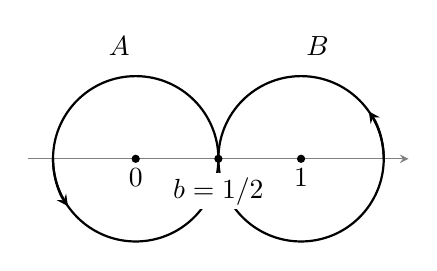
\begin{tikzpicture}[scale=2.1,>=stealth]
\draw[->,gray] (-.65,0)--(1.65,0);
\draw[thick] (0,0) circle(.5);
\draw[thick,->] (-.5,0) arc[start angle=180,end angle=215,radius=.5];
\draw[thick] (1,0) circle(.5);
\draw[thick,->] (1.5,0) arc[start angle=0,end angle=35,radius=.5];
\fill (0,0) circle(.025) node[below] {$0$};
\fill (1,0) circle(.025) node[below] {$1$};
\fill (.5,0) circle(.025) node[below=5pt,fill=white,inner sep=1.5pt] {$b=1/2$};
\node at (-.1,.68) {$A$};\node at (1.1,.68) {$B$};
\end{tikzpicture}
\end{center}
On a sheet where $L_1$ has increased by $2\pi i n$, traversal
of $A$ leaves $L_1$ unchanged and changes $F$ by
\[
\Delta_A F=-2\pi i n\oint_A\frac{dz}{z}=4\pi^2n.
\]
The principal part contributes zero because
$-\log(1-z)/z$ is analytic inside the zero circle.
For $B$, the additive constant $2\pi i n$ contributes zero
because $B$ has zero winding about zero.  To find the remaining
increment, let $L_0$ be the logarithm of $z$ analytic inside
this one-circle neighborhood, with $L_0(1)=0$.  Integration by
parts gives
\[
\Delta_B F=-[L_1L_0]_{\rm start}^{\rm end}
             +\oint_B L_0\,dL_1
           =-2\pi i\ln b+2\pi i L_0(1)
           =2\pi i\ln2.
\]
Here $L_1$ gains $2\pi i$, so $B$ also changes the integer
sheet label from $n$ to $n+1$.  Inverse loops give the inverse
increments.  It follows inductively that every word in $A,B$
ends at a value of the form
\[
\boxed{F_0+2\pi i n\ln2+4\pi^2m,\qquad m,n\in\mathbb Z}.
\]
Conversely, follow $B$, then $A$, then $B^{-1}$, then $A^{-1}$.
The two $B$ increments cancel, while $A$ was traversed with
sheet label one; this path adds $4\pi^2$ and returns the label
to zero.  Its repetitions and inverse give every $m$, after
which $B^n$ gives every $n$.  Thus the boxed set is both
necessary and sufficient, with no branch values omitted.

\erratum{The manual's proposed $2n^2\pi^2-2\pi i n\ln2$
correction is not the full branch set and is incorrect for odd
$n$.  Substituting a multivalued logarithm into the principal
reflection formula while equating its two dilogarithms assigns
incompatible branches.}  For example one loop $B$ gives
$F_0+2\pi i\ln2$ with no real shift, directly contradicting
that proposed enumeration.

\Needspace{5\baselineskip}
\par\bigskip
\noindent\textbf{18.7.4}\quad Explain why Eq.~(18.161) gives the
expected result for $z=0$ when on the principal branch of the
dilogarithm.
\solution
One cannot substitute $z=0$ separately into $\ln z$.
Take the principal-branch limit instead.  For $z\to0$ off its
logarithmic cut,
\[
\ln(1-z)=-z+O(z^2),\qquad
\ln z\ln(1-z)=-z\ln z+O(z^2\ln z).
\]
Writing $z=re^{i\theta}$ with $|\theta|\le\pi$ gives
$|z\ln z|\le r(|\ln r|+\pi)\to0$; the remainder also
vanishes.  The dilogarithm series gives
$\operatorname{Li}_2(0)=0$, while its continuous boundary value
at one is $\operatorname{Li}_2(1)=\sum n^{-2}=\pi^2/6$.
Consequently the two sides of Eq.~(18.161) both tend to
\[
\boxed{\pi^2/6}.
\]
This is a limit of the product, not an assignment of a finite
value to $\ln0$.  The principal branch condition also matters:
on other sheets the extra logarithmic terms must be continued
consistently.

\Needspace{5\baselineskip}
\par\bigskip
\noindent\textbf{18.7.5}\quad Show that
\[
\mathrm{Li}_{2}\left(\frac{1+z^{-1}}{2}\right)
=-\mathrm{Li}_{2}\left(\frac{1+z}{1-z}\right)
-\frac{1}{2}\ln^{2}\left(\frac{1-z^{-1}}{2}\right).
\]
\erratum{Exclude $z=0,1$ and use matching logarithm and dilogarithm branches.  Principal values give the identity directly for real $z>1$ or $z<0$; continue consistently elsewhere.}\par\nobreak
\solution
Set $w=(1+z^{-1})/2=(z+1)/(2z)$, with $z\ne0,1$.
Two elementary reductions are
\[
\frac{w}{w-1}
 =\frac{(z+1)/(2z)}{(1-z)/(2z)}=\frac{1+z}{1-z},
\qquad
1-w=\frac{1-z^{-1}}2.
\]
Insert them into Eq.~(18.163),
$\operatorname{Li}_2(w)+\operatorname{Li}_2(w/(w-1))
=-\tfrac12\log^2(1-w)$, and move its second term to the
right:
\[
\boxed{\operatorname{Li}_2\!\left(\frac{1+z^{-1}}2\right)
=-\operatorname{Li}_2\!\left(\frac{1+z}{1-z}\right)
-\frac12\log^2\!\left(\frac{1-z^{-1}}2\right)}.
\]
For real $z>1$ or $z<0$, both dilogarithm arguments are less
than one and the logarithm's argument is positive, so this is
an equality of ordinary real principal values.  Complex values
follow by continuing all three terms along the same path from
such a domain.

\erratum{The formula is not an unrestricted identity between
independently selected boundary values on the cut.}  For
$0<z<1$, both dilogarithm arguments exceed one, but a small
imaginary part of $z$ puts them on opposite sides of their cuts.
For example, at $z=1/3$ the arguments both equal $2$.
Selecting the same boundary value for both would incorrectly
assert $2\operatorname{Li}_2(2)=\pi^2/2$, although the boundary
values have imaginary parts $\pm\pi\ln2$.  Opposite boundary
values, with the matching logarithm, satisfy the continued identity.

\Needspace{5\baselineskip}
\par\bigskip
\noindent\textbf{18.7.6}\quad The following integral arises in the
computation of the electronic energy of the Li atom using a
correlated wave function (one that explicitly includes the
electron-electron distances as well as the distances of electrons
from the nucleus):
\[
I=\iiint d^{3}r_{1}\,d^{3}r_{2}\,d^{3}r_{3}\,
\frac{e^{-\alpha_{1}r_{1}-\alpha_{2}r_{2}-\alpha_{3}r_{3}}}
{r_{1}r_{2}r_{3}r_{12}r_{13}r_{23}},
\]
where $r_{i}=|\mathbf{r}_{i}|$,
$r_{ij}=|\mathbf{r}_{i}-\mathbf{r}_{j}|$, and the integrations are
over the entire three-dimensional space of each $\mathbf{r}_{i}$.
For convergence of $I$, we require all $\alpha_{j}>0$, but there
are no restrictions on their relative magnitudes.
\par In terms of the auxiliary quantities
\[
\zeta_{1}=\frac{\alpha_{1}}{\alpha_{2}+\alpha_{3}},\qquad
\zeta_{2}=\frac{\alpha_{2}}{\alpha_{1}+\alpha_{3}},\qquad
\zeta_{3}=\frac{\alpha_{3}}{\alpha_{1}+\alpha_{2}},
\]
this integral has the value
\[
I=\frac{32\pi^{3}}{\alpha_{1}\alpha_{2}\alpha_{3}}
\left(-\frac{\pi^{2}}{2}+\sum_{j=1}^{3}
\left[\mathrm{Li}_{2}(\zeta_{j})-\mathrm{Li}_{2}(-\zeta_{j})
+\ln\zeta_{j}\ln\left(\frac{1-\zeta_{j}}{1+\zeta_{j}}\right)\right]\right).
\]
Rearrange $I$ to a form (first found by Remiddi\footnote{E.~Remiddi, ``Analytic value of the atomic three-electron correlation integral with Slater wave functions,'' \emph{Physical Review A} \textbf{44}, 5492 (1991).}), in which
all terms in the final expression are guaranteed to evaluate to
real quantities and can be evaluated as principal values.
\erratum{In the given complex expression use continuation from $0<\zeta_j<1$, with the logarithm boundary values matching those of $\mathrm{Li}_2(\zeta_j)$.  At $\zeta_j=1$ use the finite limit.}\par\nobreak
\solution
For a positive variable $\zeta$, denote one summand by
\[
S(\zeta)=\operatorname{Li}_2(\zeta)-\operatorname{Li}_2(-\zeta)
 +\ln\zeta\log\frac{1-\zeta}{1+\zeta}.
\]
Start with $0<\zeta<1$, where all terms are real.  Reflection
and the logarithm of a positive quotient give
\[
\operatorname{Li}_2(\zeta)=\frac{\pi^2}{6}
 -\operatorname{Li}_2(1-\zeta)-\ln\zeta\ln(1-\zeta),
\]
\[
\log\frac{1-\zeta}{1+\zeta}
 =\log(1-\zeta)-\ln(1+\zeta).
\]
The terms containing $\ln\zeta\log(1-\zeta)$ cancel, leaving
\[
S(\zeta)=\frac{\pi^2}{6}
 -\operatorname{Li}_2(1-\zeta)-\operatorname{Li}_2(-\zeta)
 -\ln\zeta\ln(1+\zeta).
\]
Continue this equality consistently above or below $\zeta=1$.
The imaginary parts in the original combination cancel; the
right side is already real for every $\zeta>0$.
At $\zeta=1$ it has a finite limit, so no $0\log0$ product
needs to be evaluated separately.

Sum over $j=1,2,3$.  The three constants $\pi^2/6$ cancel
the original $-\pi^2/2$ exactly.  Thus the desired form is
\[
\boxed{I=-\frac{32\pi^3}{\alpha_1\alpha_2\alpha_3}
 \sum_{j=1}^3\left[
 \operatorname{Li}_2(-\zeta_j)+\operatorname{Li}_2(1-\zeta_j)
 +\ln\zeta_j\ln(1+\zeta_j)\right]}.
\]
The assumptions $\alpha_j>0$ imply $\zeta_j>0$.
Consequently $-\zeta_j<0$, $1-\zeta_j<1$, and both logarithm
arguments are strictly positive.  Every term in the final formula
therefore has a real principal value, for arbitrary relative
magnitudes of the three positive decay parameters.  In particular,
$\zeta_j=1$ is harmless because $\operatorname{Li}_2(0)=0$
and $\ln1=0$.

\Needspace{12\baselineskip}
\subsection*{18.8 Elliptic Integrals}

\Needspace{5\baselineskip}
\par\bigskip
\noindent\textbf{18.8.1}\quad The ellipse $x^{2}/a^{2}+y^{2}/b^{2}=1$
may be represented parametrically by $x=a\sin\theta$,
$y=b\cos\theta$. Show that the length of arc within the first
quadrant is
\[
a\int_{0}^{\pi/2}(1-m\sin^{2}\theta)^{1/2}\,d\theta=aE(m).
\]
\erratum{Take $a\ge b>0$, so $0\le m=(a^2-b^2)/a^2<1$.  The value $m=1$ is the degenerate limit $b\downarrow0$.}
\solution
Take $a\ge b>0$, so the given parameter lies in $0\le m<1$.
Differentiating the parametrization gives
$dx/d\theta=a\cos\theta$ and $dy/d\theta=-b\sin\theta$.
The arc-length element is therefore
\begin{align*}
ds&=\sqrt{(dx)^2+(dy)^2}
 =\sqrt{a^2\cos^2\theta+b^2\sin^2\theta}\,d\theta\\
 &=a\sqrt{1-\frac{a^2-b^2}{a^2}\sin^2\theta}\,d\theta.
\end{align*}
As $\theta$ increases from $0$ to $\pi/2$, the point moves
from $(0,b)$ to $(a,0)$ along precisely the first-quadrant arc.
Thus its length is
\[
\boxed{\ell=a\int_0^{\pi/2}\sqrt{1-m\sin^2\theta}\,d\theta
              =aE(m)},\qquad m=1-b^2/a^2.
\]
For $a=b$, $m=0$ and $\ell=\pi a/2$, the quarter-circle length.
The limit $b\downarrow0$ gives $m\uparrow1$ and
$\ell\to a\int_0^{\pi/2}\cos\theta\,d\theta=a$;
this is a degenerate limiting ellipse.  If $b>a$, interchange the
axis labels (or use $\theta\mapsto\pi/2-\theta$) to obtain
$bE(1-a^2/b^2)$ in the conventional nonnegative-parameter form.

\Needspace{5\baselineskip}
\par\bigskip
\noindent\textbf{18.8.2}\quad Derive the series expansion
\[
E(m)=\frac{\pi}{2}\left[1-\left(\frac{1}{2}\right)^{2}
\frac{m}{1}-\left(\frac{1\cdot3}{2\cdot4}\right)^{2}
\frac{m^{2}}{3}-\cdots\right].
\]
\erratum{The series is valid for $|m|\le1$, with the square root continued from $m=0$.}\par\nobreak
\solution
For $|m|<1$, expand the integrand uniformly in $\theta$:
\[
\sqrt{1-m\sin^2\theta}
 =1+\sum_{n=1}^\infty(-1)^n\binom{1/2}{n}
                  m^n\sin^{2n}\theta.
\]
For $n\ge1$, direct multiplication of the binomial factors gives
\[
(-1)^n\binom{1/2}{n}=-\frac{(2n-3)!!}{(2n)!!},
\]
where $(-1)!!=1$.  The sine moment is the beta integral
\[
\int_0^{\pi/2}\sin^{2n}\theta\,d\theta
 =\frac12B(n+\tfrac12,\tfrac12)
 =\frac\pi2\frac{(2n-1)!!}{(2n)!!}.
\]
Multiply these factors and use
$(2n-3)!!=(2n-1)!!/(2n-1)$:
\[
\boxed{E(m)=\frac\pi2\left[
 1-\sum_{n=1}^\infty\frac1{2n-1}
       \left(\frac{(2n-1)!!}{(2n)!!}\right)^2m^n\right]}.
\]
The first two nonconstant terms are
$-(1/2)^2m$ and $-(1\cdot3/(2\cdot4))^2m^2/3$,
which reproduce the requested series.  In ordinary powers,
\[
E(m)=\frac\pi2\left(1-\frac m4-\frac{3m^2}{64}
                             -\frac{5m^3}{256}-\cdots\right).
\]
Since $(2n-1)!!/(2n)!!\sim1/\sqrt{\pi n}$, the absolute
coefficients are $O(n^{-2})$.  Thus the series is absolutely
uniformly convergent for $|m|\le1$ and extends to the boundary
by continuity.  In particular $m=1$ gives $E(1)=1$, consistent
with its defining integral.

\Needspace{5\baselineskip}
\par\bigskip
\noindent\textbf{18.8.3}\quad Show that
\[
\lim_{m\to0}\erratum{\frac{K(m)-E(m)}{m}}
=\frac{\pi}{4}.
\]
\solution
\erratum{The original printed exercise has $(K-E)/m$, without
an extra factor $\pi$ in the numerator.  That extra factor in
the supplied transcription has been removed.  The published
erratum also makes both arguments explicitly $m$.}
Subtract the defining integrands before taking the limit:
\begin{align*}
K(m)-E(m)
 &=\int_0^{\pi/2}
 \frac{1-(1-m\sin^2\theta)}{\sqrt{1-m\sin^2\theta}}d\theta\\
 &=m\int_0^{\pi/2}\frac{\sin^2\theta}
                               {\sqrt{1-m\sin^2\theta}}d\theta.
\end{align*}
For $|m|$ bounded strictly below one, the integrand is dominated
by a constant times $\sin^2\theta$.  Dominated convergence gives
\[
\boxed{\lim_{m\to0}\frac{K(m)-E(m)}m
 =\int_0^{\pi/2}\sin^2\theta\,d\theta=\frac\pi4}.
\]
Equivalently the two series start with
$K=(\pi/2)(1+m/4+O(m^2))$ and
$E=(\pi/2)(1-m/4+O(m^2))$.
If the spurious numerator factor $\pi$ were retained, the limit
would instead be $\pi^2/4$, so it cannot accompany the stated
right side.

\Needspace{5\baselineskip}
\par\bigskip
\noindent\textbf{18.8.4}\quad A circular loop of wire in the
$xy$-plane, \erratum{centered at the origin with radius $a>0$}, carries a current $I$. Given
that the vector potential is
\[
A_{\varphi}(\rho,\varphi,z)
=\frac{a\mu_{0}I}{2\pi}\int_{0}^{\pi}
\frac{\cos\alpha\,d\alpha}
{(a^{2}+\rho^{2}+z^{2}-2a\rho\cos\alpha)^{1/2}},
\]
show that
\[
A_{\varphi}(\rho,\varphi,z)
=\frac{\mu_{0}I}{\pi k}\left(\frac{a}{\rho}\right)^{1/2}
\left[\left(1-\frac{k^{2}}{2}\right)K(k^{2})-E(k^{2})\right],
\]
where
\[
k^{2}=\frac{4a\rho}{(a+\rho)^{2}+z^{2}}.
\]
\par\emph{Note.}~For extension of this exercise to $\mathbf{B}$, see
Smythe.\footnote{W.~R.~Smythe, \emph{Static and Dynamic Electricity}, 3rd ed. (McGraw-Hill, New York, 1969), p.~270.}
\erratum{Take $\rho>0$ and real $z$, away from the wire $(\rho,z)=(a,0)$; recover the axis by a limit.}\par\nobreak
\solution
Assume $a>0$, $\rho>0$, away from the ideal wire
$(\rho,z)=(a,0)$.  Set
\[
D=(a+\rho)^2+z^2,\quad m=k^2=\frac{4a\rho}D,
\quad 0<m<1.
\]
Using $\cos\alpha=2\cos^2(\alpha/2)-1$, the denominator
squared becomes
\[
a^2+\rho^2+z^2-2a\rho\cos\alpha
 =D-4a\rho\cos^2(\alpha/2)
 =D[1-m\cos^2(\alpha/2)].
\]
Put $u=\alpha/2$ and then $\theta=\pi/2-u$:
\[
A_\varphi=\frac{a\mu_0 I}{\pi\sqrt D}
 \int_0^{\pi/2}\frac{2\sin^2\theta-1}
                         {\sqrt{1-m\sin^2\theta}}d\theta.
\]
The difference of the elliptic integrands gives
\[
K(m)-E(m)=m\int_0^{\pi/2}
 \frac{\sin^2\theta}{\sqrt{1-m\sin^2\theta}}d\theta.
\]
Therefore the remaining angular integral is
\[
\frac2m[K(m)-E(m)]-K(m)
 =\frac2m\left[(1-\tfrac m2)K(m)-E(m)\right].
\]
Finally
\[
\frac{2a}{m\sqrt D}
 =\frac1k\sqrt{\frac a\rho},
\]
because $k=2\sqrt{a\rho}/\sqrt D$.  Substitution yields
\[
\boxed{A_\varphi(\rho,\varphi,z)=\frac{\mu_0I}{\pi k}
 \sqrt{\frac a\rho}
 \left[(1-\tfrac{k^2}2)K(k^2)-E(k^2)\right]}.
\]
Rotational symmetry explains the absence of $\varphi$.
\erratum{At $\rho=0$ the apparent singular factors are interpreted
by a limit: the original integral is zero, so $A_\varphi=0$ on
the axis.  At the ideal wire $k^2=1$, the logarithmic singularity
is real and is not a removable limit.}
The cancellation near $k=0$ is also quantified by the next exercise.

\Needspace{5\baselineskip}
\par\bigskip
\noindent\textbf{18.8.5}\quad An analysis of the magnetic vector
potential of a circular current loop leads to the expression
\[
f(k^{2})=k^{-2}\big[(2-k^{2})K(k^{2})-2E(k^{2})\big],
\]
where $K(k^{2})$ and $E(k^{2})$ are the complete elliptic integrals
of the first and second kinds. Show that for $k^{2}\ll1$
($r\gg\text{radius of loop}$)
\[
f(k^{2})\approx\frac{\pi k^{2}}{16}.
\]
\erratum{Here $r=\sqrt{\rho^2+z^2}$ and the loop radius is $a$.  The far-field condition $r\gg a$ is sufficient for $k^2\ll1$.}\par\nobreak
\solution
Write $m=k^2$.  Since the definition divides by $m$, retain the
elliptic series through $m^2$ (one extra order beyond the desired
answer):
\[
K(m)=\frac\pi2\left(1+\frac m4+\frac{9m^2}{64}+O(m^3)\right),
\quad
E(m)=\frac\pi2\left(1-\frac m4-\frac{3m^2}{64}+O(m^3)\right).
\]
Then
\begin{align*}
(2-m)K(m)-2E(m)
 &=\frac\pi2\left[
 2-\frac m2+\left(\frac{18}{64}-\frac14\right)m^2
 -2+\frac m2+\frac{6m^2}{64}+O(m^3)\right]\\
 &=\frac\pi2\left[\frac{m^2}{8}+O(m^3)\right].
\end{align*}
The constant and linear terms cancel.  Dividing by $m$ gives
\[
\boxed{f(k^2)=\frac{\pi k^2}{16}+O(k^4)}.
\]
Keeping the next terms $25m^3/256$ in $2K/\pi$ and
$-5m^3/256$ in $2E/\pi$ would give
$f(m)=\pi m/16+3\pi m^2/64+O(m^3)$.
Thus $f$ has the removable value $f(0)=0$.

For the distant loop field, $D\sim r^2$,
$m\sim4a\rho/r^2$ and the preceding exercise has
$A_\varphi=a\mu_0I f(m)/(\pi\sqrt D)$.
Consequently its leading term is
$\mu_0Ia^2\rho/(4r^3)=\mu_0Ia^2\sin\theta/(4r^2)$,
the magnetic-dipole form.  Large $r/a$ is a sufficient way to
make $m$ small; it is not the only one, since $m\to0$ also
on approaching the symmetry axis.

\Needspace{5\baselineskip}
\par\bigskip
\noindent\textbf{18.8.6}\quad Show that
\begin{enumerate}
\item[(a)] $\dfrac{d\,E(k^{2})}{dk}=\dfrac{1}{k}
\big(E\erratum{(k^{2})}-K\erratum{(k^{2})}\big)$,
\item[(b)] $\dfrac{d\,K(k^{2})}{dk}
=\dfrac{E\erratum{(k^{2})}}{k(1-k^{2})}
-\dfrac{K\erratum{(k^{2})}}{k}$.
\end{enumerate}
\par\emph{Hint.}~For part (b) show that
\[
E(k^{2})=(1-k^{2})\int_{0}^{\pi/2}
(1-\erratum{k^{2}}\sin^{2}\theta)^{-3/2}\,d\theta
\]
by comparing series expansions.
\erratum{Initially take $0<k<1$; both derivatives have removable limits at $k=0$.}\par\nobreak
\solution
Take initially $0<k<1$, put $m=k^2$, and use differentiation
under the integral on compact subintervals of this range.
(a) The chain rule gives
\[
\frac{dE(k^2)}{dk}
 =-k\int_0^{\pi/2}\frac{\sin^2\theta}
                             {\sqrt{1-k^2\sin^2\theta}}d\theta.
\]
Since $-k\sin^2\theta=[(1-k^2\sin^2\theta)-1]/k$,
\[
\boxed{\frac{dE(k^2)}{dk}=\frac{E(k^2)-K(k^2)}k}.
\]

(b) First verify the corrected hint by the requested series method.
Define
\[
a_n=\left[\frac{(1/2)_n}{n!}\right]^2,
\qquad J(m)=\int_0^{\pi/2}(1-m\sin^2\theta)^{-3/2}d\theta.
\]
The binomial series and the sine moment give
\[
J(m)=\frac\pi2\sum_{n=0}^\infty
 \frac{(3/2)_n(1/2)_n}{(n!)^2}m^n
 =\frac\pi2\sum_{n=0}^\infty(2n+1)a_nm^n.
\]
For $n\ge1$, $a_n/a_{n-1}=(2n-1)^2/(4n^2)$.
Hence the $m^n$ coefficient of $2(1-m)J/\pi$ is
\[
(2n+1)a_n-(2n-1)a_{n-1}
 =a_n\left[(2n+1)-\frac{4n^2}{2n-1}\right]
 =-\frac{a_n}{2n-1}.
\]
The constant is one, so Exercise~18.8.2 identifies the entire
series with $2E(m)/\pi$.  Thus
\[
\boxed{E(m)=(1-m)J(m)},\qquad |m|<1.
\]
This uses the \erratum{corrected integrand $1-k^2\sin^2\theta$},
not $1-k\sin^2\theta$.

Now differentiate $K$ and rewrite its numerator:
\begin{align*}
\frac{dK(k^2)}{dk}
 &=k\int_0^{\pi/2}\frac{\sin^2\theta}
                              {(1-k^2\sin^2\theta)^{3/2}}d\theta\\
 &=\frac1k\int_0^{\pi/2}\left[
       \frac1{(1-k^2\sin^2\theta)^{3/2}}
       -\frac1{\sqrt{1-k^2\sin^2\theta}}\right]d\theta\\
 &=\frac{J(k^2)-K(k^2)}k
 =\boxed{\frac{E(k^2)}{k(1-k^2)}-\frac{K(k^2)}k}.
\end{align*}
All elliptic arguments in these formulas are the parameter
$k^2$, as stated in the published erratum.
At $k=0$ both derivatives have the removable value zero:
$E(k^2)=\pi/2-\pi k^2/8+O(k^4)$ and
$K(k^2)=\pi/2+\pi k^2/8+O(k^4)$.
The singular endpoint $k=1$ is outside the finite derivative
formulas and is approached only as a limit.
